% INFORMAÇÃO SOBRE A VERSÃO DESSE DOCUMENTO
% VERSÃO DA CLASSE ppgccufmg 1.60 (de 2021-03-29) - http://vilarneto.com/ppgccufmg (ou https://web.archive.org/web/20210626223024/https://vilarneto.com/ppgccufmg/)

\documentclass[msc,project]{ppgccufmg}    % ou [msc] para dissertações
                                  % de mestrado. Para propostas ou
                                  % projetos, usar [phd,project],
                                  % [msc,proposal], etc.

% \usepackage[brazil]{babel}        % se o documento for em português, OU
\usepackage[english]{babel}      % se o documento for em inglês
% \usepackage[latin1]{inputenc}
\usepackage[utf8]{inputenc}
\usepackage[T1]{fontenc}
\usepackage{type1ec}
\usepackage{amsthm}
\usepackage{graphicx}
\usepackage{pgfplots}
\usepackage[a4paper,
  portuguese,
  bookmarks=true,
  bookmarksnumbered=true,
  linktocpage,
  colorlinks,
  citecolor=black,
  urlcolor=black,
  linkcolor=black,
  filecolor=black,
  ]{hyperref}
\usepackage[square]{natbib}

\usepackage{tikz, tikz-network}

\usepackage{amsmath, amssymb, amsfonts, amsbsy, algorithmicx, algorithm}

\usepackage[noend]{algpseudocode}

\usepackage{mdframed}
\usepackage{lipsum}

\makeatletter
% \def\BState{\State\hskip-\ALG@thistlm}
\makeatother

% \newtheorem{theorem}{Theorem}
% \newtheorem{theorem}{Teorema}
% \newtheorem{lemma}{Lema}

\newtheorem{theorem}{Theorem}[chapter]
% \newtheorem{lemma}{Lemma}
\newtheorem{lemma}[theorem]{Lemma}
\newtheorem{claim}[theorem]{Claim}
\newtheorem{corollary}[theorem]{Corollary}

%%%% operadores matemáticos
\DeclareMathOperator{\opt}{\textrm{OPT}}
\DeclareMathOperator{\val}{\textrm{val}}
\DeclareMathOperator{\sol}{\textrm{Sol}}

%%% Definições
% \newcommand{\steinercycle}{\textsc{Steiner Multicycle}}

% definicoes
\newcommand{\steinercycle}{\textsc{SMCP}}
\newcommand{\steinercyclerestricted}{\textsc{R-SMCP}}
\newcommand{\steinerforest}{\textsc{SFP}}
\newcommand{\ptas}{\textsc{PTAS}}
\newcommand{\nonpoly}{\mathcal{NP}}
\newcommand{\nonpolyopt}{\mathcal{NPO}}

\newcommand{\poly}{\mathcal{P}}

\usepackage{algpseudocode}

% muda nomes de comandos do algorithmicx 
\algrenewcommand\algorithmicrequire{\textbf{Input:}}
\algrenewcommand\algorithmicensure{\textbf{Output:}}

\newenvironment{ftheo}
  {\begin{mdframed}\begin{theorem}}
  {\end{theorem}\end{mdframed}}

\newenvironment{flemma}
  {\begin{mdframed}\begin{lemma}}
  {\end{lemma}\end{mdframed}}

\newenvironment{fcorollary}
  {\begin{mdframed}\begin{corollary}}
  {\end{corollary}\end{mdframed}}

\begin{document}

% O comando a seguir, \ppgccufmg, provê todas as informações relevantes para a
% classe ppgccufmg. Por favor, consulte a documentação para a descrição de
% cada chave.

% Um exemplo para documentos em português é apresentado a seguir:
\ppgccufmg{
  title={An algorithmic study of the Steiner Multicycle Problem},
  authorrev={Martins Costa, Raul Wagner},
  %cutter={D1234p},
  %cdu={519.6*82.10},
  university={Federal University of Minas Gerais},
  course={Computer Science},
  % portuguesetitle={Um estudo algorítmico do Problema de Multiciclos de Steiner},
  portugueseuniversity={Universidade Federal de Minas Gerais},
  portuguesecourse={Ciência da Computação},
  address={Belo Horizonte},
  date={2024-02},
  % keywords={Algoritmos de Aproximação,Teoria de Grafos,Otimização,Complexidade Computacional},
  % postkeywords={Algoritmos de Aproximação,Teoria de Grafos,Otimização,Complexidade Computacional},
  % indexkeys={},
  advisor=[male]{Prof. Dr. Phablo F. S. Moura},
%   coadvisor=[female]{Maria Teresa Eleonora},
%  approval={img/approvalsheet.eps},
%  approval=[-2.5cm][1]{aprovalsheet},
  abstract={Resumo}{capitulos/abstract_port},
  abstract={Abstract}{capitulos/abstract},
%   abstract={Resumo Estendido}{capitulos/resumoest},
  % dedication={capitulos/dedicatoria},
  ack={capitulos/agradecimentos},
%  ack=[Acknowledgments]{ack},
%   epigraphtext={A verdade é o contrário da mentira, \\
%     e a mentira é o oposto da verdade.}{Autor desconhecido},
  indexkeys={1.~Computação --- Teses. 2.~Redes --- Teses. I.~Orientador.
    II.~Título.},
  beforetoc={\listofalgorithms}
}

% \keywords{}
% \keywords{Algoritmos de Aproximação, Teoria de Grafos, Otimização, e Complexidade Computacional}


% Um exemplo para documentos em inglês é apresentado a seguir (lembre-se de
% usar \usepackage[english]{babel}):
%\ppgccufmg{
%  title={Protocol for Error-Verification inside\\Totally Error-Free
%    Networks},
%  authorrev={da Camara Neto, Vilar Fiuza},
%  cutter={D1234p},
%  cdu={519.6*82.10},
%  university={Federal University of Minas Gerais},
%  course={Computer Science},
%  portuguesetitle={Protocolo para Verificação de Erros\\em Redes Totalmente
%    Confiáveis},
%  portugueseuniversity={Universidade Federal de Minas Gerais},
%  portuguesecourse={Ciência da Computação},
%  address={Belo Horizonte},
%  date={2008-03},
%  advisor={Adamastor Pompeu Setúbal},
%  approval={img/approvalsheet.eps},
%  abstract=[brazil]{Resumo}{resumo},
%  abstract={Abstract}{abstract},
%  dedication={dedicatoria},
%  ack={agradecimentos},
%  epigraphtext={Truth and lie are opposite things.}{Unknown},
%}




% \newcommand{\dummytxt}{\dummytxta\dummytxtb\dummytxtc}

\chapter{Introduction}
\label{chapter:introduction}

The Steiner Multicycle Problem (\(\steinercycle\)) was introduced by \cite{Pereira2018TheSM} in the context of vehicle routing where multiple companies must visit pickup and delivery locations. That way, a group of companies can collaborate to realize the necessary deliveries and reduce the total cost of transportation. 
Notably, they assume that the companies must make the deliveries periodically, and the size of each delivery is much smaller than the vehicles' capacities.
The interested reader may find more details about this application in \cite{Pereira2018TheSM}.

We briefly define as \textbf{cycle} a multiset of the edges of the graph, such that each associated vertex has an even degree (when accounting for edges repetition), and the associated subgraph of \(G\) is connected. We provide a more complete definition in Chapter~\ref{chapter:definitions}.

A solution to the Steiner Multicycle Problem can be represented by a single multiset that contains all the edges forming the cycles in the solution. Moreover, since a multiset of edges and the cycles induced by these edges are equivalent, throughout this work, we refer to the solution as both the multiset of edges and the subgraph of \(G\) induced by those edges interchangeably.

The solution cost is defined as the sum of all associated costs of the edges in the solution multiset.

More formally, the problem \(\steinercycle\) has as input an undirected graph \(G\) with a set of edges $E(G)$, a set \(\{T_1, \dots, T_k\}\) of pairwise disjoint subsets of vertices of \(G\) (a.k.a. \textbf{terminal sets}), and a function $c \colon E(G) \to \mathbb{R}_\ge$ that associates a crossing cost to each edge of \(G\). The goal of the problem is to find a minimum-cost set of cycles \(\mathcal{C}\), such that each terminal set \(T_i\) is contained within the same cycle.

The problem is defined below. An instance of \(\steinercycle\) and a feasible solution are depicted in Figure~\ref{fig:exem_multicycle}.

\medskip
\noindent \fbox{
	\parbox{.97\textwidth}{
		\noindent
		\textsc{Steiner Multicycle Problem (\textbf{SMCP})}\\
		\noindent
		\textbf{Instance}: A graph \(G\), $c \colon E(G) \to \mathbb{R}_\ge$, and a set \(\{T_1, \dots, T_k\}\) of pairwise disjoint subset of vertices of \(G\) (i.e. the terminals).\\
		%\noindent
		%\textbf{Parameter}: $k$.
		\noindent
		\textbf{Goal}: Find in \(G\) a minimum cost set of cycles such that all terminals in \(T_i\) belong to the same cycle.
	}
}
\medskip

\begin{figure}[H]
    \centering
\begin{tikzpicture}

\Vertex[x=0, y=2, label=$t'_3$, color=white]{A}
\Vertex[label=$t'_2$, color=white]{B}
\Vertex[x=2, y=2, color=white]{C}
\Vertex[x=2, y=0, color=white]{D}
\Vertex[x=2, y=4, label=$t_2$, color=white]{E}
\Vertex[x=4, y=2, label=$t_3$, color=white]{F}
\Vertex[x=4, y=0, color=white]{G}
\Vertex[x=6, y=2, label=$t_1$, color=white]{H}
\Vertex[x=6, y=0, label=$t'_1$, color=white]{I}

\Edge[lw=3pt, label=$e_1$, position=left](A)(B)
\Edge[lw=4pt, label=$e_2$, position=above](A)(C)
\Edge[lw=4pt, label=$e_3$, position=above](B)(D)
\Edge[lw=4pt, label=$e_4$, position=left](C)(D)
\Edge[lw=4pt, label=$e_5$, position=left](C)(E)
\Edge[lw=4pt, label=$e_6$, position=above](C)(F)
\Edge[label=$e_7$, position=above left](D)(F)
\Edge[label=$e_8$, position=above](D)(G)
\Edge[lw=4pt, label=$e_9$, position=above right](E)(F)
\Edge[lw=4pt, label=$e_{10}$, position=above](G)(I)
\Edge[lw=4pt, label=$e_{11}$, position=above left](G)(H)

\end{tikzpicture}
    \caption{An example of a viable solution for the \(\steinercycle\) considering a set of pairs of terminals \(\{\{t_1, t'_1\}, \{t_2, t'_2\}, \{t_3, t' _3\}\}\). The solution is represented by the edges in bold and corresponds to the multiset \(\{e_1, e_2, e_3, e_4, e_5, e_6, e_9, e_{10}, e_{11}, e_{10}, e_{11}\}\). The weights of the edges were omitted for simplicity.}
    \label{fig:exem_multicycle}
\end{figure}

\cite{Pereira2018TheSM} studied the problem for complete metric graphs (i.e., complete graphs that guarantee the triangular inequality for the edges costs). The authors presented a 4-approximation, a heuristic algorithm, and a mixed-integer linear formulation for the problem.
Moreover, the authors realized computational experiments comparing the proposed heuristic, called \textit{Refinement Search}, to a GRASP implementation. In summary, the results showed that the proposed heuristic reached better quality results in less time.

\citeauthor{Pereira2018TheSM} also introduced a restricted version of the Steiner Multicycle Problem (R-\(\steinercycle\)) in which every terminal set has only two vertices, one for pickup and the other for delivery. \cite{LINTZMAYER2020134} showed an equivalence between the two problems - \(\steinercycle\) and R-\(\steinercycle\) - by proposing a simple transformation from instances of the \(\steinercycle\) to R-\(\steinercycle\), which we present below. 

Let \(\mathcal{T} = \{t_1, \dots, t_\ell\}\) be a set of terminals, we create \(\ell\) new vertices \(\{u_1, \dots, u_\ell\}\). For each \(i \in \{1, \ldots, \ell\}\), we create an edge \((t_i, u_i)\) of cost zero. We define \(((u_1, t_2), \dots, (u_{\ell-1}, t_\ell), (u_\ell, t_1))\) as a sequence of terminals pairs of an instance of R-\(\steinercycle\). Note that the set of edges that forms a solution of \(\steinercycle\) with terminals of \(T\) have the same cost of a solution of R-\(\steinercycle\) after the addition of the new vertices. Given that equivalence, throughout this work, we assume that each terminal set in the \(\steinercycle\) contains exactly two vertices; i.e., we will refer to the R-SMCP as SMCP and denote terminal sets as terminal pairs.

\cite{smcp_3apx} proposed a 3-approximation for complete metric graphs, which is based on a 2-approximation for the Survivable Network Design Problem and the concept of T-joins, a generalization of the well-known perfect matching. This algorithm is inspired by the results obtained for the metric Travelling Salesman Problem (TSP) by \cite{Christofides2022WorstCaseAO}.

It is also essential to notice that, even for the restricted case, the Steiner Multicycle Problem is \(\nonpoly\)-hard. This can be verified by reducing the Travelling Salesman Problem (TSP) to the R-\(\steinercycle\) using a strategy similar to the one presented by \citeauthor{LINTZMAYER2020134}.

This work proposes a \textbf{polynomial-time approximation scheme} (PTAS) for the \(\steinercycle\) on a special class of graphs called \textit{bounded genus graphs}, a generalization the well-known class of planar graphs.

This work is structured as follows: Chapter~\ref{chapter:definitions} introduces some basic definitions in Graph Theory and Approximation Algorithms, as well as some definitions used to present and prove the results of this work. Chapter~\ref{chapter:related_work} overviews the literature for \(\steinercycle\) and related problems. Chapters~\ref{chapter:pc-partition} and~\ref{chapter:spanner} introduce some tooling necessary for achieving the PTAS. Next, Section~\ref{section:ptas_bounded_tree} of Chapter~\ref{chapter:apx_schemes_for_smcp} proves a PTAS for bounded treewidth graphs, which is an essential result to prove the PTAS for bounded genus graphs in the Section~\ref{section:ptas_bounded_genus} of the same chapter. Chapter~\ref{chapter:experiments} presents some experimental results of the 3-approximation algorithm proposed by \cite{smcp_3apx}. Finally, Chapter~\ref{chapter:conclusion} delivers general remarks on this work and proposes possible paths for future works.

\section{Algorithm Overview}

As we shall see, the proposed PTAS for \steinercycle\ is inspired by the PTAS for the Steiner Tree Problem due to \cite{Bateni}. Put briefly, the proposed algorithm for \steinercycle\ consists of the following steps:

\begin{enumerate}
    \item The algorithm receives as input a graph \(G_{in}\) with bounded-genus, and a set \(\mathcal{D} = \{T_1, \dots, T_k\}\) of terminal pairs.

    \item It begins by creating a spanner subgraph (i.e., a subgraph whose size is bounded by a constant time \(\opt\) and has a valid solution with a cost at most \((1 + \epsilon) \opt\) of \(G_{in}\). This is done with an auxiliary clustering algorithm provided by Theorem~\ref{chapter:pc-partition}.
    
    \item The edges of the spanner are split into \(k\)-disjoint sets, then the edges in the smallest set are contracted. After the contraction, the algorithm applies \citeauthor{Demaine2010}'s Theorem (\cite{Demaine2010} Theorem~1.1) to convert the spanner subgraph to a bounded treewidth graph.

    \item A dynamic programming algorithm is used to solve the SMCP in the bounded treewidth graph generated in the previous step. During this process, the algorithm only considers a subset of the possible solutions that organize the set of unpaired terminals (from the bottom-up in the dynamic programming tree) in valid ways.

    \item Finally, it constructs the final solution, i.e., the PTAS for bounded genus, by leveraging the solution in bounded-treewidth and the set of edges contracted in the previous step.
\end{enumerate}
\chapter{Definitions}
\label{chapter:definitions}

In this chapter we present the definitions and notations used in this work. The definitions shown are based on \cite{BondyNMurty} and \cite{Diestel}.

% Neste capítulo apresentamos as definições e notações usadas nesse trabalho. As definições apresentadas são baseadas em \cite{BondyNMurty} e \cite{Diestel}.

\section{Graphs Notation}

A graph is a pair \(G = (V, E)\) of sets satisfying \(E \subseteq [V]^2\); therefore the elements of \(E\) are subsets of \(V\) with two elements. These two sets can be observed as points and lines connecting points, respectively.

% Um grafo é um par \(G = (V, E)\) de conjunto que satisfazem \(E \subseteq [V]^2\); portanto os elementos de \(E\) são subconjuntos de \(V\) com dois elementos. Esses dois conjuntos podem ser observados como pontos e linhas que conectam pontos, respectivamente.

The set of vertices of a graph is denoted as \(V(G)\) and the set of edges as \(E(G)\). We say that \(v\) belongs to the graph \(G\) following the notation \(v \in V(G)\), and equivalently for an edge \(e\) we denote \(e \in E(G)\). We can also represent vertices and edges using \(v \in G\) or \(e \in G\), in situations where the context clarifies the nature of the treated variable.

% O conjunto de vértices de um grafo é denotado como \(V(G)\) e o conjunto de arestas como \(E(G)\). Dizemos que \(v\) pertence ao grafo \(G\) seguindo a notação \(v \in V(G)\), e de maneira equivalente para uma aresta \(e\) denotamos \(e \in E(G)\). Também podemos representar vértices e arestas usando \(v \in G\) ou \(e \in G\), em situações em que o contexto esclarece a natureza da variável tratada.

A vertex \(v\) is \textbf{incident} to an edge \(e\) if \(v \in e\); so \(e\) is an edge connected to \(v\). The two vertices incident to \(e\) are called the \textbf{endpoints} of \(e\). Another notation used to represent an edge is \(vw \in E(G)\), where \(v, w \in V(G)\) are the endpoints.

% Um vértice \(v\) é \textbf{incidente} a uma aresta \(e\) se \(v \in e\); assim \(e\) é uma aresta conectada à \(v\). Os dois vértices incidentes à \(e\) são chamados de \textbf{extremidades} de \(e\). Outra notação usada para representar uma aresta é \(vw \in E(G)\), onde \(v, w \in V(G)\) são as extremidades. 

The number of vertices of a graph is its \textbf{order}, denoted by \(|G|\). The number of edges is its \textbf{size} and is denoted by \(||G||\).

% O número de vértices de um grafo é a sua \textbf{ordem}, denotado por \(|G|\). O número de arestas é o seu \textbf{tamanho} e é denotado por \(||G||\).

Two vertices \(u\), \(v\) of \(G\) are \textbf{adjacent}, or neighbors, if there is \(e \in E(G)\) such that \(u\) and \(v\) are its endpoints. Two edges \(e\) and \(f\) are adjacent if they have one of their endpoints in common.

% Dois vértices \(u\), \(v\) de \(G\) são \textbf{adjacentes}, ou vizinhos, se existe \(e \in E(G)\) tal que \(u\) e \(v\) são suas extremidades. Duas arestas \(e\) e \(f\) são adjacentes se possuem um dos seus extremos em comum.


Let \(v \in V(G)\) be a vertex. We denote as \(N(v)\) the \textbf{open neighborhood} of \(v\), that is, the set of all vertices \(w \in V(G)\) such that \(w\) is adjacent to \(v\). The \textbf{closed neighborhood} of \(v\), denoted as \(N[v]\) is \(N(v) \cup \{v\}\).

% Seja \(v \in V(G)\) um vértice. Denotamos como \(N(v)\) a \textbf{vizinhança aberta} de \(v\), ou seja, o conjunto de todos vértices \(w \in V(G)\) tal que \(w\) é adjacente à \(v\). A \textbf{vizinhança fechada} de \(v\), denotada como \(N[v]\) é \(N(v) \cup \{v\}\).

If for any vertices \(u, v \in V(G)\) there is an edge \(uv \in E(G)\) then we say that \(G\) is a \textbf{complete} graph. A complete graph of \(n\) vertices is denoted as \(K^n\).

% Se para quaisquer vértices \(u, v \in V(G)\) existe uma aresta \(uv \in E(G)\) então dizemos que \(G\) é um grafo \textbf{completo}. Um grafo de \(n\) vértices completo é denotado como \(K^n\).

The \textbf{degree} of a vertex \(v\) is the number of edges of \(G\) incident to \(v\), denoted by \(d(v)\). Note that \(d(v) = |N(v)|\) if the graph has no loops or multiple edges. Let \(v\) be a vertex such that \(d(v) = 0\), we say that \(v\) is an \textbf{isolated vertex}. The number \(\delta(G) := \min \{d(v) \colon v \in V(G)\}\) is the \textbf{minimum degree} of \(G\), the number \(\Delta(G) := \max \{d(v) \colon v \in V(G)\}\) is the \textbf{maximum degree} of \(G\).

% O \textbf{grau} de um vértice \(v\) é o número de arestas de \(G\) incidentes à \(v\), denotado por \(d(v)\). Note que \(d(v) = |N(v)|\) se o grafo não possui laços nem arestas múltiplas. Seja \(v\) um vértice tal que \(d(v) = 0\), dizemos que \(v\) é um \textbf{vértice isolado}. O número \(\delta(G) := \min \{d(v) \colon v \in V(G)\}\) é o \textbf{grau mínimo} de \(G\), o número \(\Delta(G) := \max \{d(v) \colon v \in V(G)\}\) é o \textbf{grau máximo} de \(G\).

We say that a graph \(H = (V' , E')\) is \textbf{subgraph} of \(G\) if \(V' \subseteq V\) and \(E' \subseteq E\), that is, \(H \subseteq G\). If for any vertices \(v, w \in H \subset G\) the statement \(vw \in E(H)\) is valid if and only if \(vw \in E(G)\), then we say that \(H\) is an \textbf{induced subgraph} of \(G\), and we denote it by \(G[H]\). We say that \(H\) is a \textbf{spanning subgraph} of \(G\) if \(V' = V\).

% Dizemos que um grafo \(H = (V' , E')\) é \textbf{subgrafo} de \(G\) se \(V' \subseteq V\) e \(E' \subseteq E\), ou seja, \(H \subseteq G\). Se para quaisquer vértices \(v, w \in H \subset G\) for válida a afirmação \(vw \in E(H)\) se, e somente se, \(vw \in E(G)\), então dizemos que \(H\) é um \textbf{subgrafo induzido} de \(G\), e o denotamos por \(G[H]\). Dizemos que \(H\) é um \textbf{subgrafo gerador} de \(G\) caso \(V' = V\).

A \textbf{path} in a graph \(G\) is a sequence of distinct vertices \(P = v_1, v_2, \dots, v_k\), \(P \subseteq V(G)\), such that for every pair of consecutive vertices of \(P\), there is an edge in \(E(G)\) that connects these vertices, that is, for every \(v_i , v_{i+1}\) in \(P\), there is \(v_i v _{i+1} \in E(G)\). The number of vertices in the path is its length, and a path of length \(k\) is denoted by \(P^k\).

% Um \textbf{caminho} em um grafo \(G\) é uma sequência de vértices \(P = v_1, v_2, \dots, v_k\) distintos, \(P \subseteq V(G)\), tal que para todo par de vértices consecutivos de \(P\), existe uma aresta em \(E(G)\) que conecta esses vértices, ou seja, para todo \(v_i , v_{i+1}\) em \(P\), existe \(v_i v _{i+1} \in E(G)\). O número de vértices no caminho é o seu comprimento, um caminho de comprimento \(k\) é denominado \(P^k\).

If \(P = v_1, v_2 \dots, v_k\) is a path such that \(|P| \geq 3\) and the endpoints of the sequence \(P\) are equal, that is, \(v_1 = v_k\) , then we say that \(P\) is a \textbf{cycle}. The number of vertices of a cycle is its \textbf{length}, a cycle of length \(k\) is called \(C^k\). However, in this work, we relax the definition of cycle for the sake of simplicity. We define a cycle as a multiset of edges such that every vertex of \(G\), that is endpoint to some edge in the multiset, has even degree considering all edges in the multiset. 

% Se \(P = v_1, v_2 \dots, v_k\)  é um caminho tal que \(|P| \geq 3\) e os extremos da sequência \(P\) são iguais, ou seja, \(v_1 = v_k\) , então dizemos que \(P\) é um \textbf{ciclo}. O número de vértices de um ciclo é o seu \textbf{comprimento}, um ciclo de comprimento \(k\) é denominado \(C^k\). Neste trabalho, a definição de ciclos apresentada será relaxa permitindo a repetição de vértices. Isso é feito a fim de adequar melhor a definição do SMCP.

If there is a partition of \(V(G)\) into subsets \(V_1 , V_2 , \dots, V_w\) such that two vertices \(u\) and \(v\) are connected if, and only if, \(u\) and \(v\) belong to the same subset \(V_i\), then we say that the subgraphs \(G[V_1], G[V_2], \dots, G[V_w]\) are the \textbf{components} of \(G\). If \(G\) contains a single component, we say that \(G\) is \textbf{connected}, otherwise \(G\) is \textbf{disconnected}.

% Se existir uma partição de \(V\) em subconjuntos \(V_1 , V_2 , \dots, V_w\) tal que dois vértices \(u\) e \(v\) estão conectados se, e somente se, \(u\) e \(v\) pertencem ao mesmo subconjunto \(V_i\). Os subgrafos \(G[V_1], G[V_2], \dots, G[V_w]\) são as \textbf{componentes} de \(G\). Se \(G\) contém uma única componente, dizemos que \(G\) é \textbf{conexo}, caso contrário \(G\) é \textbf{desconexo}.

Let \(e \in E(G)\), denote by \(G / e\) the graph obtained from \(G\) by \textbf{contracting} the edge \(e\) at a new vertex \(v_e\), which becomes adjacent to all old neighbors of the endpoint vertices of \(e\).

% Seja \(e \in E(G)\), denotamos por \(G / e\) o grafo obtido a partir de \(G\) ao \textbf{contrair} a aresta \(e\) em um novo vértice \(v_e\), que se torna adjacente a todos os antigos vizinhos dos vértices extremidade de \(e\).

We define \(c \colon E(G) \to \mathbb{R}_\ge\), for \(e \in E(G)\) as the \textbf{cost} of \(e\). Equivalently \(c(H)\) for \(H \subset G\) is the sum of the cost of the edges of the subgraph \(H\). Let \(C = \{v_1, v_2, \dots, v_k\}\) be a cycle of \(G\), and there may be repetition of vertices in \(C\). We define \(c(C) = \sum_{i=1}^{k-1} c(v_i v_{i+1})\). Note that the same edge can be counted more than once in the cost calculation.

% Definimos \(c \colon E(G) \to \mathbb{R}_\ge\), para \(e \in E(G)\) como o \textbf{custo} de \(e\). De maneira equivalente \(c(H)\) para \(H \subset G\) é a soma do custo das arestas do subgrafo \(H\). Seja \(C = \{v_1, v_2, \dots, v_k\}\) um ciclo de \(G\), podendo haver repetição de vértices em \(C\). Definimos \(c(C) = \sum_{i=1}^{k-1} c(v_i v_{i+1})\). Note que uma mesma aresta pode ser contabilizada mais de uma vez no cálculo do custo.

For vertices \(v, w \in V(G)\) we define the distance between vertices $v$ and $w$, denoted by \(dist_G(v, w)\), as the length of the shortest path between \(v\) and \(w\) in \(G\). If such a path does not exist, by convention we consider \(dist_G(v, w) = +\infty\). We generalize the notation for distances between vertices and edges. Let \(v \in V(G)\) and \(uw \in E(G)\) define the distance between the vertex \(v\) and the edge \(uw\) as \(dist_G(v, uw) := \min\{dist_G(v, u), dist_G(v, w)\} + c(uw)\).

% Para vértices \(v, w \in V(G)\) definimos a distância entre os vértices $v$ e $w$, denotado por \(dist_G(v, w)\), como o comprimento do caminho mais curto entre \(v\) e \(w\) em \(G\). Caso tal caminho não exista, por convenção, consideramos \(dist_G(v, w) = +\infty\). Generalizamos a notação para distâncias entre vértices e arestas. Seja \(v \in V(G)\) e \(uw \in E(G)\) definimos a distância entre o vértice \(v\) e a aresta \(uw\) como \(dist_G(v, uw) := \min\{dist_G(v, u), dist_G(v, w)\} + c(uw)\).

We say that a graph \(F\) without cycles is a \textbf{forest}. A connected forest is a \textbf{tree}. Let \(T\) be a tree and \(v \in T\) a vertex, if \(d(v) = 1\), we say that \(v\) is a \textbf{leaf} of \(T \), all other vertices are called inner vertices of \(T\). A tree is rooted if one of its vertices has been chosen as \textbf{root}.

% Dizemos que um grafo \(F\) sem ciclos é uma \textbf{floresta}. Uma floresta conexa é uma \textbf{árvore}. Seja \(T\) uma árvore e \(v \in T\) um vértice, se \(d(v) = 1\), dizemos que \(v\) é uma \textbf{folha} de \(T\), todos demais vértices são chamados de vértices internos de \(T\). Uma árvore é enraizada se um dos seus vértices foi eleito como \textbf{raiz}.

Let \(T\) be a rooted tree with root \(r \in V(T)\), let \(v \in V(T)\), let \(P\) be the path between \(v\) and \(r\). we say that \(w \in V(T)\) is the parent vertex of \(v\) if \(w \in P\) and \(w \in N(v)\). Equivalently, we say that \(v\) is a child vertex of \(w\). Note that a vertex can have multiple children, but only one parent.

% Seja \(T\) uma árvore enraizada com raiz \(r \in V(T)\), seja \(v \in V(T)\), seja \(P\) o caminho entre \(v\) e \(r\). dizemos que \(w \in V(T)\) é o vértice pai de \(v\) se \(w \in P\) e \(w \in N(v)\). De maneira equivalente, dizemos que \(v\) é um vértice filho de \(w\). Note que um vértice pode ter múltiplos filhos, mas somente um pai.

Informally, we say that if a graph \(G\) can be drawn on a plane without its edges intersecting, then it is \textbf{planar}. Thus, the graph can be seen as points on a surface with arcs connecting the points. The surface region completely surrounded by arcs is called \textbf{face} of the graph. In particular, the outer region of the graph is the \textbf{outer face}, while all other faces are \textbf{inner faces} of \(G\). The boundary of \(G\), i.e. the set of edges that separate the outer face of \(G\) from the rest of the graph, is called \(\partial(G)\).

% De maneira informal, dizemos que se um grafo \(G\) é \textbf{planar} se pode ser desenhado em um plano sem que suas arestas se cruzem. Sendo assim, o grafo pode ser visto como pontos em uma superfície com arcos conectando os pontos. A região da superfície completamente circundada de arcos é denominada \textbf{face} do grafo. Em particular, a região exterior do grafo é a \textbf{face externa}, ao passo que todas outras faces são \textbf{faces internas} de \(G\). A fronteira de \(G\), ou seja o conjunto de arestas que separam a face externa de \(G\) do restante do grafo, é denominada \(\partial(G)\).

Formally, \cite{Diestel} defines a planar graph as a pair \((V, E)\) of finite sets with the following properties:

\begin{itemize}
    \item \(V \subseteq \mathbb{R}^2\);
    \item every edge is an arc between two vertices;
    \item different edges have different set of extreme points;
    \item the interior of an edge does not contain vertices or intersections with other edges.
\end{itemize}

% Formalmente, \cite{Diestel} define um grafo planar como um par \((V, E)\) de conjuntos finitos com as seguintes propriedades:

% \begin{itemize}
%     \item \(V \subseteq \mathbb{R}^2\);
%     \item toda aresta é um arco entre dois vértices;
%     \item diferentes arestas tem diferentes conjunto de pontos extremais;
%     \item o interior de uma aresta não contém vértices e nem intersecções com outras arestas.
% \end{itemize}

For any planar graph the set \(\mathbb{R}^2 \backslash G\) is open and its regions are the faces of \(G\).

Informally we say that the \textbf{genus} of a graph is the smallest number \textit{g} such that the graph can be drawn on a sphere with \textit{g} holes without their edges crossing. Therefore, a planar graph has genus 0. The problem of determining the genus of a graph is known to be \(\nonpoly\)-complete, as demonstrated by \cite{THOMASSEN1989568}. However, as presented by \cite{LinearGenus}, the problem becomes treatable with genus \textit{g} fixed, that is, we can determine in polynomial time whether a graph can be embedded in a surface with genus \textit{g}, considering \textit{g} constant.

% Para qualquer grafo planar o conjunto \(\mathbb{R}^2 \backslash G\) é aberto e suas regiões são as faces de \(G\).

% Informalmente dizemos que o \textbf{genus} de um grafo é o menor número \textit{g} tal que o grafo pode ser desenhado em uma esfera com \textit{g} buracos sem que as suas arestas se cruzem. Sendo assim, uma grafo planar tem \textit{genus} 0. Sabe-se que o problema de determinar o \textit{genus} de um grafo é \(\nonpoly\)-completo, como demonstrado por \cite{THOMASSEN1989568}. Entretanto, como apresentado por \cite{LinearGenus}, o problema passa a ser tratável com \textit{genus} \textit{g} fixo, ou seja, podemos determinar em tempo polinomial se um grafo pode ser incorporada em uma superfície com \textit{genus} \textit{g}, considerando \textit{g} constante.

For a given planar graph \(G\) we say that \(H\) is its \textbf{dual} if there is a bijective function that maps the faces of \(G\) to the vertices of \(H\). Furthermore, for each edge \(e \in E(G)\) that separates the faces \(f\) and \(f'\) of \(G\), we have an edge that connects the vertices referring to \(f\) and \(f'\) in \(H\).

% Para um dado grafo planar \(G\) dizemos que \(H\) é seu \textbf{dual} se existe uma função bijectiva que mapeia as faces de \(G\) à vértices de \(H\). Além disso, para cada aresta \(e \in E(G)\) que separa as faces \(f\) e \(f'\) de \(G\), temos uma aresta que conecta os vértices referentes à \(f\) e \(f'\) em \(H\) .

As defined by \cite{ROBERTSON1986309}, a \textbf{tree decomposition} of \(G\) is a pair \((T, B)\) in which \(T\) is a tree and \(B = \{B_i \colon i \in V(T)\}\) is a family of subsets of \(V(G)\) such that:

\begin{itemize}
    \item \(\bigcup_{i \in V(T)} B_i = V(G)\)
    \item For each edge \(uv \in E(G)\), there is \(i \in V(T)\) such that \(u, v \in B_i\)
    \item The set of vertices \(\{i \in V(T) \colon v \in B_i\}\) forms a subtree of \(T\) for each \(v \in V(G)\)
\end{itemize}

% Conforme definida por \cite{ROBERTSON1986309}, uma \textbf{decomposição em árvore} de \(G\) é um par \((T, B)\) no qual \(T\) é uma árvore e \(B = \{B_i \colon i \in V(T)\}\) é uma família de subconjuntos de \(V(G)\) tal que:

% \begin{itemize}
%     \item \(\bigcup_{i \in V(T)} B_i = V(G)\)
%     \item Para cada aresta \(uv \in E(G)\), existe \(i \in V(T)\) tal que \(u, v \in B_i\)
%     \item O conjunto de vértices \(\{i \in V(T) \colon v \in B_i\}\) formam uma subárvore de \(T\) para cada \(v \in V(G)\)
% \end{itemize}

To differentiate from the original graph \(G\), we call the vertices of \(T\) \textbf{nodes}, where each node \(i\) has a \textbf{bag} of vertices \(B_i\) corresponding. An example can be seen in Figure \ref{fig:decomp1} where Item (a) is a graph and (b) is a possible tree decomposition for the graph.

% Para diferenciar do grafo original \(G\), chamamos os vértices de \(T\) de \textbf{nós}, onde cada nó \(i\) possui uma \textbf{sacola} de vértices, ou simplesmente \textit{bag}, \(B_i\) correspondente. Um exemplo pode ser observado na Figura \ref{fig:decomp1} onde o Item (a) é um grafo e (b) é uma possível decomposição em árvore para o grafo.

\begin{figure}[H]
    \centering
    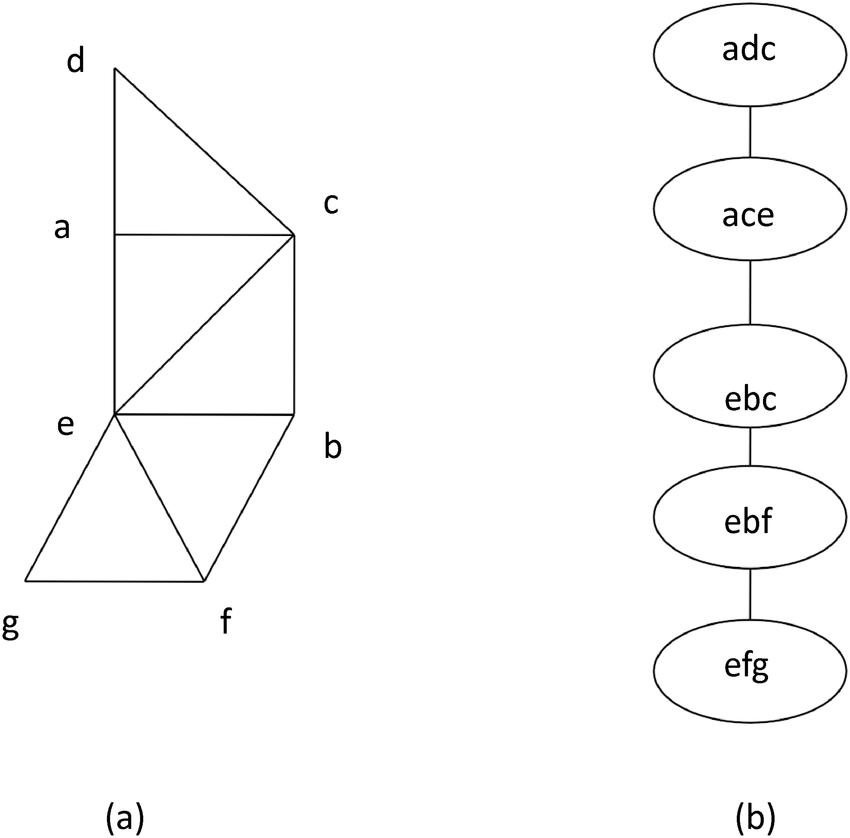
\includegraphics[scale=2]{imgs/decomp1.png}
    \caption{Example of graph and its tree decomposition. (\cite{imgTreeDecomp}).}
    \label{fig:decomp1}
\end{figure}

\begin{tikzpicture}

\Vertex[x=0, y=0, label=$g$, position=below, color=white, size=0.5]{G}
\Vertex[x=1, y=0, label=$f$, position=below, color=white, size=0.5]{F}
\Vertex[x=0.5, y=1, label=$e$, position=left, color=white, size=0.5]{E}
\Vertex[x=1.5, y=1, label=$b$, position=right, color=white, size=0.5]{B}
\Vertex[x=0.5, y=2, label=$a$, position=left, color=white, size=0.5]{A}
\Vertex[x=1.5, y=2, label=$c$, position=right, color=white, size=0.5]{C}
\Vertex[x=0.5, y=3, label=$d$, position=left, color=white, size=0.5]{D}

\Edge(A)(C)
\Edge(A)(D)
\Edge(A)(E)
\Edge(B)(C)
\Edge(B)(E)
\Edge(B)(F)
\Edge(C)(D)
\Edge(E)(F)
\Edge(E)(G)
\Edge(F)(G)

\end{tikzpicture}

\begin{tikzpicture}

\draw[label=$a$] (0, 0) ellipse (.8 and 0.5);
\draw (0, 1.5) ellipse (.8 and 0.5);
\draw (0, 3) ellipse (.8 and 0.5);
\draw (0, 4.5) ellipse (.8 and 0.5);
\draw (0, 6) ellipse (.8 and 0.5);

\draw (0, 0.5) -- (0, 1);
\draw (0, 2) -- (0, 2.5);
\draw (0, 3.5) -- (0, 4);
\draw (0, 5) -- (0, 5.5);

\end{tikzpicture}

% usar subfigures para colocar as imagens um do lado do outro

The \textbf{width} of a tree decomposition is the size of its largest bag minus one. The \textbf{tree width} of a graph \(G\), denoted with \(tw(G)\), is the smallest width of a tree decomposition of \(G\).

To facilitate application in algorithms, we focus on a more restricted class of decompositions. We say that a tree decomposition \((T, B)\) is \textbf{nice} when \(T\) is a rooted tree and each \(i \in V(T)\) belongs to one of the following classes:

% A \textbf{largura} de uma decomposição em árvore é o tamanho da sua maior sacola menos um. A \textbf{largura de árvore}, ou largura arbórea, de um grafo \(G\),  denotada com \(tw(G)\), é a menor largura de uma decomposição arvórea de \(G\).

% Para facilitar a aplicação em algoritmos, focamos em uma classe mais restrita de decomposições. Dizemos que uma decomposição em árvore \((T, B)\) é agradável, ou \textit{nice}, quando \(T\) é uma árvore enraizada e cada \(i \in V(T)\) pertence a uma das seguintes classes:

\begin{itemize}
    \item \(i\) is a leaf node if it has no children;
    \item \(i\) is a union node if \(i\) has exactly two children \(i_1, i_2\) and is worth \(B_i = B_1 = B_2\);
    \item \(i\) is an introduction node if it has a single child \(i'\) and is valid \(B_i = B_{i'} \cup \{v\}\) for some vertex \(v \in V(G)\);
    \item \(i\) is a forgetting node if it has a single child \(i'\) and holds \(B_i = B_{i'} \backslash \{v\}\) for some vertex \(v \in V(G)\).
\end{itemize}

% \begin{itemize}
%     \item \(i\) é um nó folha se não tiver nenhum filho;
%     \item \(i\) é um nó de união se \(i\) tiver exatamente dois filhos \(i_1, i_2\) e vale \(B_i = B_1 = B_2\);
%     \item \(i\) é um nó de introdução se tiver um único filho \(i'\) e vale \(B_i = B_{i'} \cup \{v\}\) para algum vértice \(v \in V(G)\);
%     \item \(i\) é um nó de esquecimento se tiver um único filho \(i'\) e vale \(B_i = B_{i'} \backslash \{v\}\) para algum vértice \(v \in V(G)\);
% \end{itemize}

\section{Classes of Optimization Problems}

In combinatorial optimization problems, we want to obtain the best solution out of a finite, but potentially large, set of possible solutions. \cite{livroAprox} defined an optimization problem with the following elements: a set of instances, a set \(\sol(I)\) of viable solutions for a given instance \(I\) and a function \(\val (I, S)\) that associates for each instance and solution \(S \in \sol(I)\) a non-negative rational value. Therefore, the solution to the optimization problem is the \(S\) that minimizes/maximizes \(\val(I, S)\).

% Em problemas de otimização combinatória, desejamos obter a melhor solução dentro de um conjunto finito, mas potencialmente grande, de soluções possíveis. \cite{livroAprox} definiram um problema de otimização com os seguintes elementos: um conjunto de instâncias, um conjunto \(\sol(I)\) de soluções viáveis para uma dada instância \(I\) e uma função \(\val(I, S)\) que associa para cada instância e solução \(S \in \sol(I)\) um valor racional não-negativo. Sendo assim, a solução do problema de otimização é o \(S\) que minimiza/maximiza \(\val(I, S)\).


More formally, for a given instance \(I\) there is a solution \(S^* \in \sol(I)\) such that \(\val(I, S^*) \leq \val(I, S)\) for all \(S \in \sol(I)\), considering a minimization scenario. The idea follows in an equivalent way for a maximization problem. We denote \(\opt := \val(I, S^*)\) as the optimal solution of \(I\). In particular, for the problems discussed in this work, we denote as \(\opt_{\mathcal{T}}(G)\) an optimal solution in the graph \(G\) considering a set of pairs of terminals \(\mathcal{T}\).

% Mais formalmente, para uma dada instância \(I\) existe uma solução \(S^* \in \sol(I)\) tal que \(\val(I, S^*) \leq \val(I, S)\) para todo \(S \in \sol(I)\), considerando um cenário de minimização. A ideia segue de maneira equivalente para um problema de maximização. Denotamos \(\opt := \val(I, S^*)\) como a solução ótima de \(I\). Em particular, para os problemas comentados nesse trabalho, denotamos como \(\opt_{\mathcal{T}}(G)\) uma solução ótima no grafo \(G\) considerando um conjunto de pares de terminais \(\mathcal{T}\).

As will be seen throughout the section, there is an intimate relationship between the classes of optimization problems and the well-known classes of decision problems: \(\poly\), \(\nonpoly\), \(\nonpoly\)-hard, \(\nonpoly\)-complete. There are optimization problems in which there is limitations of the approximability of their solutions by polynomial algorithms, considering \(\poly \neq \nonpoly\).

% Como será observado ao longo da seção, existe uma relação íntima entre as classes de problemas de otimização e as conhecidas classes de problemas de decisão: \(\poly\), \(\nonpoly\), \(\nonpoly\)-difícil, \(\nonpoly\)-completo. Existem problemas de otimização em que aparecem limitações da aproximalidade de suas soluções por algoritmos polinomiais, considerando \(\poly \neq \nonpoly\).

In this way, optimization problems are classified according to their degree of approximability. When talking about approximation, we are observing a scenario in which we give up finding the optimal solution in favor of finding a solution efficiently, while maintaining quality guarantees. In this work we will consider and detail the classes PO, FPTAS, PTAS, APX and NPO, as described by \cite{bookAprox}.

% Dessa forma, problemas de otimização são classificados conforme seu grau de aproximabilidade. Ao falar de aproximabilidade, estamos observando um cenário em que abrimos mão de encontrar a solução ótima para uma dada instância em favor de encontrar uma solução de maneira eficiente, mas mantendo garantias de qualidade. Neste trabalho vamos considerar e detalhar as classes PO, FPTAS, PTAS, APX e NPO, conforme descrito por \cite{livroAprox}.

According to \citeauthor{bookAprox}, the NPO class, which is an extension of the \(\nonpoly\) class for optimization problems, is composed of the problems where:

\begin{itemize}
    \item There is a polynomial function \textit{p} such that \(\langle S \rangle \leq p\langle\langle I\rangle\rangle\) for every instance \(I\) of the problem and every feasible solution \( S\) of \(I\);
    \item There is a polynomial algorithm that decides whether a given word is a valid representation of an instance of the problem;
    \item There is a polynomial algorithm that decides whether a given object is a viable solution for a given instance of the problem;
    \item There is a polynomial algorithm that calculates \(\val(I, S)\), given \(I\) and \(S\).
\end{itemize}

% De acordo com \citeauthor{livroAprox}, a classe NPO, que é uma extenção da classe \(\nonpoly\) para problemas de otimização, é composta pelos problemas em que:

% \begin{itemize}
%     \item Existe uma função polinomial \textit{p} tal que \(\langle S \rangle \leq p\langle\langle I\rangle\rangle\) para toda instância \(I\) do problema e toda solução viável \(S\) de \(I\);
%     \item Existe uma algoritmo polinomial que decide se uma dada palavra é uma representação válida de uma instância do problema;
%     \item Existe um algoritmo polinomial que decide se um dado objeto é solução viável de uma dada instância do problema;
%     \item Existe um algoritmo polinomial que calcula \(\val(I, S)\), dados \(I\) e \(S\).
% \end{itemize}

We denote as PO the class of problems treatable in polynomial time. This class is an extension of the P class for optimization problems. Therefore, given a problem \(\pi\), we say that \(\pi \in PO\) if there is a polynomial algorithm that calculates an optimal solution for each instance \(I\) of \(\pi\). Examples of problems of this class are the Shortest Path and Minimum Spanning Tree problems.

% Denotamos como PO a classe de problemas tratáveis em tempo polinomial. Esta classe é uma extensão da classe P para problemas de otimização. Sendo assim, dado um problema \(\pi\), dizemos que \(\pi \in PO\) se existe um algoritmo polinomial que calcular uma solução ótima para cada instância \(I\) de \(\pi\). Exemplos de problemas dessa classe são os problemas de Caminho Mínimo e de Árvore Geradora Mínima.

Consider an optimization problem. Let \(A\) be an algorithm in which for every viable instance \(I\) of the problem returns a viable solution \(A(I)\) of \(I\). If the problem is one of minimization and \(A(I) \leq \alpha \opt\) holds for every instance \(I\), then we say that \(A\) is a \(\alpha\)-approximation of the problem. We denote \(\alpha\) as \textbf{approximation ratio} of the algorithm.

% Considere um problema de otimização. Seja \(A\) um algoritmo em que para toda instância \(I\) viável do problema devolve uma solução viável \(A(I)\) de \(I\). Se o problema é de minimização e vale \(A(I) \leq \alpha \opt\) para toda instância \(I\), então dizemos que \(A\) é uma \(\alpha\)-aproximação do problema. Denotamos \(\alpha\) como \textbf{razão de aproximação} do algoritmo.

The APX class is composed of optimization problems in NPO for which there is a \(\alpha\)-polynomial-time approximation for some constant \(\alpha\). One of the most famous algorithms that provides this type of approximation is the Christofides Algorithm, developed by \cite{Christofides2022WorstCaseAO} to the TSP problem restricted to metric graphs and which guarantees an approximation with \(\alpha = 1.5\).

% A classe APX é composta por problemas de otimização em NPO para os quais existe uma \(\alpha\)-aproximação em tempo polinomial para alguma constante \(\alpha\). Um dos algoritmos mais famosos que fornece esse tipo de aproximação é o Algoritmo de Christofides, desenvolvido por \cite{Christofides2022WorstCaseAO} e que garante uma aproximação com \(\alpha = 1,5\) para o problema do TSP restrito à grafos métricos.

For a given optimization problem, we define as an \textbf{approximation scheme} an algorithm that receives an instance \(I\) of the problem as well as a parameter \(0 < \ epsilon < 1\) and returns a solution \(S\) such that \(\val(I, S) \leq (1 + \epsilon) \opt\), for a minimization problem. We say that an algorithm is a \textbf{polynomial-time approximation scheme} (PTAS), if it is polynomial for every fixed \(\epsilon\). Furthermore, an algorithm is a \textbf{full polynomial-time approximation scheme}, or FPTAS, if it is also polynomial in \(1 / \epsilon\), whereas a PTAS algorithm, which is not FPTAS, is exponential in \(1 / \epsilon\).

% Para um dado problema de otimização, definimos como um \textbf{esquema de aproximação}, ou do inglês \textit{approximation scheme}, um algoritmo que recebe uma instância \(I\) do problema assim como um parâmetro \(0 < \epsilon < 1\) e retorna uma solução \(S\) tal que \(\val(I, S) \leq (1 + \epsilon) \opt\), para um problema de minimização. Dizemos que um algoritmo é um \textbf{esquema de aproximação em tempo polinomial}, ou \textit{polynomial-time approximation scheme} (PTAS), se ele é polinomial para todo \(\epsilon\) fixo. Além disso, um algoritmo é um \textbf{esquema de aproximação em tempo polinomial pleno}, ou FPTAS, se ele também é polinomial em \(1 / \epsilon\), ao passo que um algoritmo PTAS, mas não FPTAS, é exponencial em \(1 / \epsilon\).

From the definitions it follows that $$PO \subseteq FPTAS \subseteq PTAS \subseteq APX \subseteq NPO.$$

Equivalent to decision problems, we also have the idea of a problem being NPO-hard, that is, \(PO = NPO\) if and only if \(\poly = \nonpoly\). Therefore, a problem is NPO-hard if it is NPO and its decision version is \(\nonpoly\)-complete. So we have the concept of the \textbf{inapproximability} of a problem.

% De maneira equivalente a problemas de decisão, também temos a ideia de um problema ser NPO-difícil, ou seja \(PO = NPO\) se e somente se \(\poly = \nonpoly\). Sendo assim, um problema é NPO-difícil se for NPO e sua versão de decisão for \(\nonpoly\)-completo. Assim temos o conceito da \textbf{inaproximabilidade} de um problema.

Despite belonging to APX when restricted to metric graphs, the TSP problem is NPO-hard in general graphs. That is, if TSP is in APX, then \(\poly = \nonpoly\). This result has been observed and demonstrated for TSP, and other problems of interest, in \cite{NPOcompleteApproxProblems}.

Equivalently, we also observe APX-hard problems, i.e. if \(\poly = \nonpoly\) then PO = NPO, as noted by \cite{ComplexityApproximation}.

% Apesar de pertencer à APX quando restrito a grafos métricos, o problema TSP é NPO-difícil em grafos gerais. Ou seja se TSP está em APX, então \(\poly = \nonpoly\). Esse resultado foi observado e demonstrado para o TSP, e outros problemas de interesse, em \cite{NPOcompleteApproxProblems}.

% De maneira equivalente, também observamos problemas APX-difíceis. Vale notar que se \(\poly = \nonpoly\) então PO = NPO, conforme observado por \cite{ComplexityApproximation}.

\chapter{Related Work}
\label{chapter:related_work}


The Steiner Multicycle Problem (\(\steinercycle\)) is related to vehicle routing problems, particularly pickup and delivery problems. The literature for this class of problems is vast and considers multiple different restrictions and scenarios (\cite{surveyRouter}).

The \(\steinercycle\) stands between (and generalizes) two big classes of problems that are of much interest to the optimization and theoretical computing communities: the Traveling Salesman Problem (TSP) and the Steiner Tree Problem (STP).

We start this chapter by diving into the literature on the TSP, and some of its variants. We then move to the STP and discuss some of its variants that are more related to this study. 
Our literature review of these problems focuses on approximation algorithms, and more specifically on PTASes.

\section{Travelling Salesman Problem}

One of the most studied vehicle routing optimization problem is the Travelling Salesman Problem or TSP. In this problem, we aim to find a minimal-cost Hamiltonian cycle (i.e., a closed cycle that visits each vertex exactly once) in a given graph.

As mentioned in Chapter~\ref{chapter:introduction}, we can draw a link between the TSP and the \(\steinercycle\), since an instance of the TSP can be converted in polynomial time to an instance of the \(\steinercycle\). That is, the TSP is a particular case of the \(\steinercycle\).

The \textbf{Christofides Algorithm}, proposed by \cite{Christofides2022WorstCaseAO}, is one of the most famous approximation algorithms for the TSP. This algorithm is a \(3/2\)-approximation on metric graphs.

\cite{williamsonApxAlgs} present the following summary of the algorithm. Given a metric graph \(G\), we calculate its minimum spanning tree \(M\). Let \(O\) be the set of odd-degree vertices in \(M\). By the Handshaking Lemma, there are an even number of odd-degree vertices in \(M\). One of the classic results in combinatorial optimization is that given a complete graph (on an even number of vertices), it is possible to calculate a perfect matching of minimum total cost in polynomial time. Considering that, we can calculate it for \(O\). If we add the edges of the perfect matching over \(O\) in \(M\), we create an Eulerian multigraph \(H\) since it is connected and all vertices have even degrees. Finally, we can shortcut the duplicated edges to create a solution of no greater cost corresponding to a Hamiltonian cycle.

Interestingly, more than four decades of research failed to improve upon \citeauthor{Christofides2022WorstCaseAO}' \(3/2\) factor, until \cite{slightlyBetterApxTSP} provided a randomized \((3/2 - \epsilon)\)-approximation for \(\epsilon > 10^{-36}\). Their method follows similar principles to \citeauthor{Christofides2022WorstCaseAO}' algorithm but uses a randomly chosen tree from a carefully selected random distribution in place of the minimum spanning tree.

It is generally known that finding PTASes is difficult for a lot of problems. In particular, \cite{noPTASMetricTSP} showed that there is no PTAS for metric TSP, as well as for the Steiner Tree Problem, Maximum Directed Cut Problem (in which we want to find a bipartition of the vertices of the graph such that the cost of the edges crossing the partition is maximum), and Shortest Superstring Problem (in which we want to find a shortest possible string that contains every string in a given set as substrings), unless \(\poly = \nonpoly\).

\cite{PTASeuclidianTSP} designed a PTAS for \textbf{Euclidean TSP}. They strategy consisted in recursively partitioning the plane (using a randomized variant of the quadtree) such that some \((1 + \epsilon)\)-approximate salesman tour crosses each line of the partition at most \(\mathcal{O}(1/\epsilon)\) times. Such a tour is found by dynamic programming. For each line in the partition, the algorithm first ``guesses'' where the tour crosses this line and the order in which those crossings occur. Then it recurses independently on the two sides of the line. Only \(n \log{n}\) distinct regions are in the partition, where \(n\) is the number of nodes in the plane. Furthermore, the “guess” can be fairly coarse, so the algorithm spends only \(\mathcal{O}(\log{n})^{\mathcal{O}(1/\epsilon)}\) time per region, for a total running time of \(n \cdot (\log{n})^{\mathcal{O}(1/\epsilon)}\). The result still holds even if the nodes are in \(\mathbb{R}^d\), but the running time increases to \(\mathcal{O}(n (\log{n})^{(\mathcal{O}(\sqrt{dc}))^{d-1}})\).

One of the few practical implementations of a PTAS in the literature was done by \cite{implementationPTASeuclidianTSP} for \citeauthor{PTASeuclidianTSP}'s algorithm. Their work describes an implementation of the Euclidean TSP that is based on the essential steps of \citeauthor{PTASeuclidianTSP}'s PTAS with some additional heuristics to improve the running time. In general, their results showed that this PTAS can achieve good performance in practice, although due to challenges during implementation, the authors had to make decisions that caused the loss of theoretical guarantees of the solution's quality. This illustrates how challenging implementing a PTAS can be.

\cite{baker1994} presented a method for obtaining PTASes for a variety of optimization problems in planar graphs, e.g. maximum-weight independent set and minimum-weight vertex cover. This method was generalized by \cite{demaine2005} to derive algorithms for nonlocal problems, such as feedback vertex set and connected dominating set. They were able to derive approximation schemes for subclasses of minor-excluded graphs that involve turning the input graph into a low-treewidth graph. That way, their results apply to graphs that are not planar.

\cite{KleinTSP} improved the results from the work of \cite{basicPTASplanarTSP} by generating an EPTAS for TSP in planar graphs. 
To do so, the authors proposed a framework based on the results from \cite{baker1994} and \cite{demaine2005}, which consists of the following steps.

The first step creates a subgraph \(H\) called \textbf{spanner}.
A spanner \(H\) has two properties of interest: the Quasi-optimality property, which means there is a solution of cost \((1 + \epsilon) \opt\) in \(H\) and the Shortness property, which means the cost of \(H\) is bounded by a constant times \(\opt\). The second step is to find a set of edges of cost at most \(\mathcal{O}(\epsilon \opt)\) contained in \(H\), then proceed to contract those edges. According to~\cite{Demaine2010}, the resulting graph of this process has bounded treewidth. The third step uses a dynamic programming approach on this bounded treewidth graph to obtain an optimal solution. Finally, the solution is the union of the resulting graph from the dynamic programming with the set of edges that was contracted.

\cite{KleinTSP} also showed that this framework could be generalized to obtain PTASes for multiple problems in planar graphs. \cite{Bateni} even commented: ``Most approximation schemes for planar graph problems use (implicitly or explicitly) the fact that the problem is easy to solve on bounded-treewidth graphs''. That fact is the basis for his work on the Steiner Forest Problem (which will be presented later in this chapter).

\cite{EPTASeuclidianTSP} improved on \cite{PTASeuclidianTSP} work by using ``light'' spanners for Euclidean graphs to obtain an EPTAS for Euclidean TSP.~\cite{contraction-decomposition-in-h-minor-free-graphs} proved that any graph excluding a fixed minor can have its edges partitioned into a desired number \(k\) of color classes such that contracting the edges in any one color class results in a graph of treewidth linear in \(k\). This result allowed them to generalize \citeauthor{KleinTSP}'s framework to H-minor-free graphs. Given that, and using the spanners proposed by~\cite{light_spanners_tsp}, \citeauthor{contraction-decomposition-in-h-minor-free-graphs} proposed the first PTAS for TSP in weighted H-minor-free graphs. This result improved upon the early work by~\cite{light_spanners_tsp}, who designed a QPTAS for the same problem.

Since \citeauthor{light_spanners_tsp}'s spanner has weight \(\mathcal{O}(\log{(n)} \; \mathrm{poly}(1 / \epsilon)) \opt\), \citeauthor{contraction-decomposition-in-h-minor-free-graphs}'s PTAS is not efficient.~\cite{eptas-tsp-h-minor-free} improved on the spanner's size resulting in an EPTAS for the problem. The authors mentioned that designing a PTAS for the Subset TSP (also known as Steiner Cycle Problem) in H-minor-free graphs is a central open problem of the field (we will present more on this ahead).

Two related problems to the TSP are the \textbf{Steiner Cycle Problem} and the \textbf{Multiple Steiner Cycle Problem}. These will be presented in the next section.

\section{Steiner-related problems}

We loosely define a ``Steiner-related'' problem as any problem that aims at making some kind of connection between terminals inside one or more sets of vertices. Traditionally, these connections are made with trees or cycles.

During this section, we will present some relevant results in the literature for a few Steiner-related problems, in particular the Steiner Tree Problem, Steiner Cycle Problem, the Steiner Forest Problem, and the Multiple Steiner Traveling Salesman Problem. At the end of the section, we will present some results for the \(\steinercycle\).

\subsection{Steiner Tree Problem}

The Steiner Tree Problem (STP) is one of the most studied problems in the combinatorial optimization literature. The problem consists of finding a tree with minimum cost that connects a subset of the vertices, called terminals, in the graph. It was one of the \(\nonpoly\)-complete problems presented by~\cite{Karp1972}.

In their work,~\cite{Borradaile2009b} drew inspiration from~\cite{KleinTSP} framework to create a PTAS for the Steiner Tree Problem in planar graphs. The authors built a spanner using a subgraph \(MG\), called Mortar Graph, and a set of \textbf{bricks} - subgraphs that are only connected to the rest of the graph via a bounded set of vertices called \textbf{portals}. More details of those concepts are given ahead. This spanner would suffice to be applied to \citeauthor{KleinTSP}'s framework to obtain a PTAS, but it was noted by the authors that such PTAS would yield a time complexity double exponential on \(1 / \epsilon\).

To improve this result, the authors decomposed \(MG\) into a set of subgraphs called \textbf{parcels}. This decomposition was done via a breadth-first search in the dual of \(MG\). As a result, each parcel is an embedded planar subgraph of \(MG\). From this, the authors defined a simple graph called \textbf{parcel graph} in which each vertex represents a parcel in \(MG\).

The constructed parcel graph has some interesting properties, one of which is that the planar dual of each parcel has a spanning tree with depth limited by a constant. That way, they can compute the optimal Steiner Tree for each parcel and take their union to obtain a solution for the original graph. This new approach resulted in a running time singly exponential in \(\mathrm{poly}(1 / \epsilon)\).

To use the Mortar Graph to build the spanner, the authors presented and demonstrated a structural theorem that guarantees that the optimal solution found in the Mortar Graph, and its bricks, is at most \((1 + \epsilon) \opt\).

\subsection{Steiner Cycle Problem}

The \(\steinercycle\) was also studied in a more restricted variant, where we must cover all terminals with a single cycle. This more restricted problem is known in the literature as \textbf{Steiner Cycle Problem}, SCP (it is also known as \textbf{Steiner TSP} or \textbf{Subset TSP}). It is possible to observe that the SCP is equivalent to the TSP in the scenario where all vertices are terminals.

\cite{Cornuejols1985} first introduced the SCP (named Steiner TSP by the authors) while studying the problem in its graphical case and investigating its polyhedron in series–parallel graphs.

\cite{SalazarSteinerCycle} analyzed the polyhedral structure associated with the Steiner Cycle Problem and introduced two lifting strategies to generate inequalities facet defining based on the TSP polytope.

\cite{SteinovaSteinerCycle} presented a 3/2-approximation for the SCP in metric graphs. The authors also showed that there is no constant time approximation for general graphs unless \(\poly = \nonpoly\). This result implies that the SCP, and by consequence the \(\steinercycle\), is NPO-hard in general graphs.

\cite{Arora1998APA} found a \textit{quasipolynomial-time approximation scheme} for the SCP in planar graphs. To find a \((1 + \epsilon)\)-approximated solution for the problem, the proposed algorithm requires time \(\mathcal{O}(n^{\mathrm{poly}(\log n, 1/\epsilon)})\). They made the following conjecture that allows the derivation of a PTAS from this result: ``There exists a function \(f(\cdot)\) such that given \(\epsilon > 0\), a planar graph \(G\) with edge-weights, and a subset \(S\) of vertices, there exists an edge-induced subgraph \(G'\) that \((1 + \epsilon)\)-approximates all distances between nodes in \(S\), and furthermore, \(G'\) has total edge weight at most \(f(\epsilon)\) times the minimum Steiner tree weight for \(S\).''

\cite{klein2006} created a PTAS for SCP in planar graphs, the first one proposed for the problem, by following up from \cite{Arora1998APA}. They confirmed \citeauthor{Arora1998APA}'s conjecture to be true by showing a constructive proof that implies a polynomial-time algorithm for the construction of the subgraph \(G'\), i.e., the \textbf{spanner}.

\cite{klein2014} proposed a sub-exponential parameterized algorithm for the problem with time complexity \((2^{\mathcal{O}(\sqrt{k} \log{k})} + W) \cdot n^{\mathcal{O}(1)}\), where \(n\) is the number of vertices and \(k\) is the numbers of terminals, if \(G\) is a planar graph with weights that are integers no greater than \(W\). The primary strategy to achieve this result consists of two steps: (1) find a locally optimal solution and (2) use it to guide a dynamic program. The proof of correctness of the algorithm depends on the treewidth of a graph obtained by combining an optimal solution with a locally optimal solution.

\cite{LeSubsetTspPTAS_H_MinorFree} proposed a PTAS for the SCP in H-minor-free graphs, for any fixed graph \(H\), expanding on \cite{eptas-tsp-h-minor-free} work. Their main contribution is the concept of a nearly light subset spanner construction based on sparse spanner oracles. They show that spanner oracles with weak sparsity are necessary and sufficient to construct light subset spanners, even for general graphs.

This result is interesting for several reasons. Despite the many advances in meta-algorithms related to PTAS in H-minor-free graphs, a PTAS for SCP on this class of graphs was still unknown. Moreover, there is evidence that a PTAS for this problem is impossible in more general graphs than H-minor-free.


\subsection{Multiple Steiner Traveling Salesman Problem}

The \textbf{Multiple Steiner Traveling Salesman Problem with Order Constraints}, or briefly MSTSPO, is a close variant of the Steiner Multicycle Problem. The difference is that the MSTSPO fixes a set of \(K\) salesman, each having to visit a set of terminals to form the cycles, and considers that each cycle must visit the terminals in a predefined order.

% S. Borne, A. R. Mahjoub, and R. Taktak. A branch-and-cut algorithm for the multiple steiner  TSP with order constraints.
\cite{BORNE2013487} formulated the problem motivated by survivability issues in multilayer telecommunication networks as Multiple Steiner TSP with Order Constraints. Their work proposes an integer linear programming formulation for the problem and investigates the associated polytope. They also present new valid inequalities and discuss their facial aspect. Finally, they devised a Branch-and-cut algorithm and presented preliminary computational results.

% The Multiple Steiner TSP with order constraints: complexity and optimization algorithms
\cite{Gabrel2020} expanded on \citeauthor{BORNE2013487}'s work by proposing a few integer programming formulations and both Branch-and-Cut and Branch-and-Price algorithms to solve the problem. They presented extensive computational results, showing the efficiency of the algorithms.

\subsection{Steiner Forest Problem}

Another \(\steinercycle\) related problem is the Steiner Forest Problem (SFP), where instead of using cycles to connect terminal pairs, we restrict ourselves to using only trees. In a similar way that the \(\steinercycle\) generalizes the SCP, the SFP generalizes the STP. 

\cite{Bateni} proposed a PTAS for the Steiner Forest Problem based on the work of \cite{Borradaile2009b}. To do so, the authors presented a clustering algorithm called \textbf{Prize Collecting Clustering}, which aims at segmenting the original graph in a set of trees \(\{T_1, \dots, T_k\}\) in such a way that the sum of the cost of all trees is at most \((4/\epsilon + 2) \opt\), where \(\opt\) is the cost of an optimal solution for the entire graph, encompassing all terminal sets.

Besides that, considering \(\mathcal{D}_i\) as a set of terminals that must be connected, and \(T_i\) as the tree that connects the terminals in \(\mathcal{D}_i\), the sum of the costs of all the minimal Steiner Forests, connecting only the vertices within each \(\mathcal{D}_i\), totals at most \((1 + \epsilon) \opt\). That can be expressed as \(\sum_i \opt_{\mathcal{D}_i} \leq (1 + \epsilon) \opt\).

In simpler terms, the union of optimal solutions for each terminal set forms an \(1 + \epsilon\)-approximated solution for the input graph. Finally, for each tree \(T_i\) obtained by the clustering, the authors applied the framework proposed by \cite{KleinTSP}, and expanded by \cite{Borradaile2009b, Borradaile2012}.

\subsection{Steiner Multicycle Problem}

// TODO reescrever para ficar diferente da introdução

\cite{LINTZMAYER2020134} proposed the first PTAS for the \(\steinercycle\). The algorithm is a randomized PTAS restricted to the Euclidean plane. In this context, the Euclidean \(\steinercycle\) encompasses a set of terminal pairs distributed across a plane and aim to calculate the line segments that connect the points with the least cost, considering that the same line segment might be crossed more than once.

The algorithm groups the terminal pairs in such a way that pairs that are far away from each other belong to different groups. The authors guarantee that the union of the optimal solution calculated in each group is bounded by a constant times the optimal solution when considering all terminal pairs. Then, for each group of terminal pairs, they create a square called \textbf{root dissection square}, which is a bounding box containing all terminal pairs of the group. This square has a cost of at most a constant times the optimal solution cost considering the terminals pairs in the square.

For each square, they run a process of recursive dissection. In this process, each square is subdivided into four squares of equal size, using vertical and horizontal lines. They select a limited number of points in its border as portals, for each generated square during the partitioning. That way, the solutions generated by the algorithm cross the squares only through the portals. At the end of the process, each square that has not been partitioned is broken into cells, like in a grid. 

For each square \(R\), the authors define a memoization table \(M_R\), indexed by valid configurations of \(R\), in other words, valid subpartitions of the cells and portals of \(R\). Considering a valid configuration of \(R\) called \(\pi\), \(M_R(\pi)\) is the cost of the minimal solution that is \textbf{compatible} with \(\pi\) and \textbf{conforms} to \(R\). A solution is compatible with \(\pi\) when its line segments respect the partition of \(\pi\) and a solution conforms with \(R\) when it is feasible, connects the necessary terminal pairs, only crosses the borders in \(R\) through portals, and makes that crossing a limited number of times.

To write an entry in \(M_R(\pi)\), the authors observe all possible configurations of the squares generated by subdividing \(R\), the ``children'' squares of \(R\), and only consider entries consistent with \(\pi\) from all these configurations. They show that the combined solutions of the four ``children'' squares generate a solution compatible with \(\pi\) and conform to \(R\).

\cite{smcp_3apx} presented a 3-approximation for \(\steinercycle\) on metric and complete graphs. The algorithm was based on the work done by \cite{Christofides2022WorstCaseAO} for the metric TSP and consists of the following three basic steps.
The first step is to perform a 2-approximation for the Survivable Network Design Problem (SNDP), considering a specific set of parameters which will be detailed next. The authors described the SNDP as follows: given a graph \(G\), a weight function \(w: E(G) \rightarrow \mathbb{Q}_+\), and a non-negative integer \(r_{ij}\) for each pair of vertices \(i\), \(j\) with \(i \neq j\), representing a connectivity requirement, the goal is to find a minimum weight subgraph \(G'\) of \(G\) such that, for every pair of vertices \(i, j \in V(G)\) with \(i \neq j\), there are at least \(r_{ij}\) edge-disjoint paths between \(i\) and \(j\) in \(G'\).

They also observed that given an \(\steinercycle\) instance, it is easy to define an equivalent SNDP instance by considering \(r_{ij} = 2\) for any vertices \(i\) and \(j\) that belong to the same terminal set and \(r_{ij} = 0\) otherwise. That way, the optimum value of the SNDP is also a lower bound on the optimum for the Steiner Multicycle Problem: indeed, an optimal solution for the Steiner Multicycle Problem is a feasible solution for the SNDP with the same cost. Those parameters of the SNDP are used on the first step of the algorithm.

Let \(T\) be a set of vertices that has an even number of elements in \(G\). A set \(J\) of edges in \(G\) is a \textbf{T-join} if the set of vertices of \(G\) that are incident to an odd number of edges in \(J\) is exactly \(T\).

Let \(G'\) be the output of the 2-approximation for the SNDP. Consider \(T\) to be the set of odd-degree vertices in \(G'\). Thus, the second step of the algorithm consists of calculating in polynomial time a minimum \(T\)-join \(J\) in \(G'\). Finally, as the third step, we obtain an Eulerian graph \(H\) from \(G'\) by doubling the edges in \(J\) and, by shortcutting an Eulerian tour for each component of \(H\), one obtains a collection \(C\) of cycles in \(G\) that is the output of the algorithm.


\cite{Borradaile2012} expanded the works of \cite{Borradaile2009b} and \cite{KleinTSP} to obtain PTASes in subset connectivity problems in bounded-genus graphs. To do that, the authors proposed two methods. The first method is a generalization of the Mortar Graph framework by \cite{KleinTSP}. The second applies the strategy proposed in \cite{Borradaile2009b}, but using the simpler tree decomposition instead of the parcel decomposition.

// TODO escrever overview aqui

In this work, we intend to expand on the results found by \cite{LINTZMAYER2020134} by proposing a PTAS for the \(\steinercycle\) in graphs with bounded-genus. To that end, we will use various techniques proposed by \cite{Bateni} and \cite{Borradaile2009b} for the Steiner Forest and Steiner Tree problems, respectively, such as the Mortar Graph, the Prize Collecting Clustering, and the spanner.

\chapter{Computational Experiments}
\label{chapter:experiments}

We ran computational experiments in two distinct algorithms on instances for the Steiner Multicycle Problem (SMCP). In particular, we implemented the \(3\)-approximation algorithm proposed by \cite{smcp_3apx}, and a relaxed solver to obtain a lower bound to optimal results for the same instances.

It is worth mentioning that we initially tried to run an exact solver to obtain the optimal solutions, but the execution time became prohibitive for this strategy.

# TODO add as footnote
All experiments were executed in an Intel Core i5 11400H with a 16Gb 3200MHz RAM. The code was compiled with Clang version 15.0.1 on a Windows 10 machine. You can see the code at: https://github.com/RaulWCosta/steiner-multicycle-problem-3-apx

The algorithms were implemented in C++ using the Graph library \cite{lemon} and the \cite{gurobi}.

The linear relaxation was implemented using \cite{Pereira2018TheSM} formulation. From \citeauthor{Pereira2018TheSM}, given an instance \((G, c, T)\) of the SMCP, consider a function \(f: 2^V \rightarrow \{0, 1\}\) such that for each non-empty set \(S \subset V\) we have \(f(S) = 1\) if, and only if, there is some \(T_a \in \mathcal{T}\) such that \(S \cap T_a \neq \emptyset\) and \(T_a \nsubseteq S\), i.e., \(S\) is a cut that separates terminals in \(T_a\). They use \(i \in T\) to denote a vertex in a terminal. The SMCP can be formulated as:

\begin{align}
&\text{minimize} &\sum_{e\in E} c_e x_e \label{form-pereira:1}\\
&\text{subject to} &\sum_{e \in \delta(i)} x_e &= 2 &&\text{\(\forall i \in \mathcal{T}\)} \label{form-pereira:2}\\ 
&&\sum_{e \in \delta(S)} x_e &\geq 2 f(S) &&\text{\(\emptyset \neq S \subset V\)} \label{form-pereira:3}\\ 
&&x_e &\in \{0, 1, 2\} &&\text{$e \in E(G)$} \label{form-pereira:4}
\end{align}

Where \(\delta(S)\) denotes the set of edges having exactly one endpoint in \(S\). The variable \(x_e\) indicates if an edge is used in the solution, Constraint~\eqref{form-pereira:2} assures that exactly one cycle covers each terminal, Constraint~\eqref{form-pereira:3} assures that vertices belonging to a terminal set \(T_a \in \mathcal{T}\) are connected, and Constraint~\eqref{form-pereira:4} allows each edge to be used at most twice.

By relaxing the integrality Constraint~\eqref{form-pereira:4} we obtain the linear program used in the implementation. Note that the number of constraints~\eqref{form-pereira:3} is exponential. However, we managed to compute the relaxed LP in polynomial time by using Gomory-Hu trees to solve maximum flow problems between each pair of vertices in the same terminal set \(T_a\). This is the same strategy employed by \cite{Pereira2018TheSM} on their implementations.

# TODO parei aqui

\section{3-approximation Algorithm}

As presented in Section~\ref{subsection:steinermulticycle}, \cite{smcp_3apx} proposed the following algorithm to obtain a 3-approximation for SMCP.

\begin{algorithm}
\caption{SMCP 3-approximation}
\label{algorithm:smcp-3-apx}
\begin{algorithmic}[1]

\Require A complete graph \(G\), a weight function \(w: E(G) \rightarrow \mathbb{Q}_+\) satisfying the triangle inequality, and a partition \(\mathcal{T} = \{T_1, \dots, T_k\}\) of \(V(G)\)

\Ensure A collection \(\mathcal{C}\) of cycles that respects \(\mathcal{T}\)

\State \(r_{i, j} \gets 2\) for every \(i, j \in T_a\) for some \(1 \leq a \leq  k\)
\State \(r_{i, j} \gets 0\) for every \(i \in T_a\) and \(j \in T_b\) for some \(1 \leq a < b \leq k\).
\State \(G' \gets 2ApproxSND(G, w, r)\) \label{alg:3-apx:snd-2-apx}
\State Let \(T\) be the set of odd degree vertices in \(G'\)
\State Let \(w'\) be the restriction of \(w\) to the edges in \(G'\)
\State \(J \gets MinimumTJoin(G', w', T)\) \label{alg:3-apx:t-join}
\State \(H \gets G' + J\)
\State \(\mathcal{C} \gets ShortCutting(H)\) \label{alg:3-apx:shortcutting}
\State return \(\mathcal{C}\)


\end{algorithmic}
\end{algorithm}


% \begin{enumerate}
%     \item Perform a 2-approximation for the Survivable Network Design Problem (SNDP) in \(G\) to find a subgraph \(G'\)
%     \item Calculate a minimum \(T\)-join \(J\) in \(G'\).
%     \item Create an Eulerian graph \(H\) by doubling each edge of \(J\) and adding them to \(G'\).
%     \item Shortcut an Eulerian tour for each component of \(H\) to obtain a collection \(C\) of cycles in \(G\), which is the algorithm's output.

% \end{enumerate}

To calculate the SNDP in line~\eqref{alg:3-apx:snd-2-apx}, we implemented the 2-approximation proposed by \cite{snd-2-apx}. This algorithm solves the linear relaxation of the problem and rounds the solutions. We also used Gomory-Hu trees to add cuts to the linear relaxation at each iteration.

As mentioned by the authors, Theorem~1 from \cite{smcp_3apx} implies that a minimum weight perfect matching in the graph \(G[T]\) weights at most \(w(G')/2\). This means that one can exchange line~\eqref{alg:3-apx:t-join} to compute, instead, a minimum weight perfect matching \(J\) in \(G[T]\). We applied this strategy in our implementation.

The shortcutting in line~\eqref{alg:3-apx:shortcutting} is done by finding any Eulerian cycle within each component of \(H\). We conjecture that the quality of the 3-approximation could be further improved by adopting a better strategy for shortcutting, at the cost of a potentially greater execution time.

\section{Instances}

As of the time of writing, the only experimental study available for the SMCP (more specifically, its restricted version R-SMCP) was the one presented by \cite{Pereira2018TheSM}. In their work, they evaluated implementations of their proposed algorithm and a well-known metaheuristic using two instance types. Type 1 is a set of instances from the multi-commodity one-to-one pickup-and-delivery traveling salesman problem (m-PDTSP), and type 2 is a set of randomly generated instances created by them.

\cite{HERNANDEZPEREZ2009987} generated a set of instances to the m-PDTSP. For each instance, they generated \(2n - 2\) uniformly random points with coordinates from \(-500\) to \(500\), a vertex in position \(0\) with coordinates \((0, 0)\) and a vertex in position \(2n - 1\) also with coordinates \((0, 0)\) (corresponding to Class 3 of \cite{HERNANDEZPEREZ2009987}). Like \cite{Pereira2018TheSM}, we only consider the vertex distribution of these instances. For each \(i \in \{0, \dots, n - 1\}\), we assign a vertex \(i\) as a pickup point of an agent and \(i + n\) as its corresponding delivery point. The instances have 6, 11, and 16 agents, totaling 210 instances. This set of instances is of the type 1.

\cite{Pereira2018TheSM} generated a set of instances having 16, 32, 64, 128, and 256 agents, where vertices correspond to points distributed in a square of dimensions \(100000\) by \(100000\). The square is divided into \(1 \times 1\), \(2 \times 2\), \(3 \times 3\), \(4 \times 4\), and \(5 \times 5\) frames, and each pair of pickup and delivery is in the same frame. The space between frames, which we call a wall, has \(0\%\), \(10\%\), \(20\%\), \(30\%\), or \(40\%\) of the frame’s size. The wall can be seen as a rectangle separating the different frames (see Figure~\ref{fig:instances_type_2}). Notice that there is no wall for the instances with division \(1 \times 1\). The location of each point is chosen uniformly at random. For each combination of the number of agents, frames, and wall size, three instances were generated with different seeds, therefore, 315 instances of type 2 were generated.

\begin{figure}[H]
    \centering
    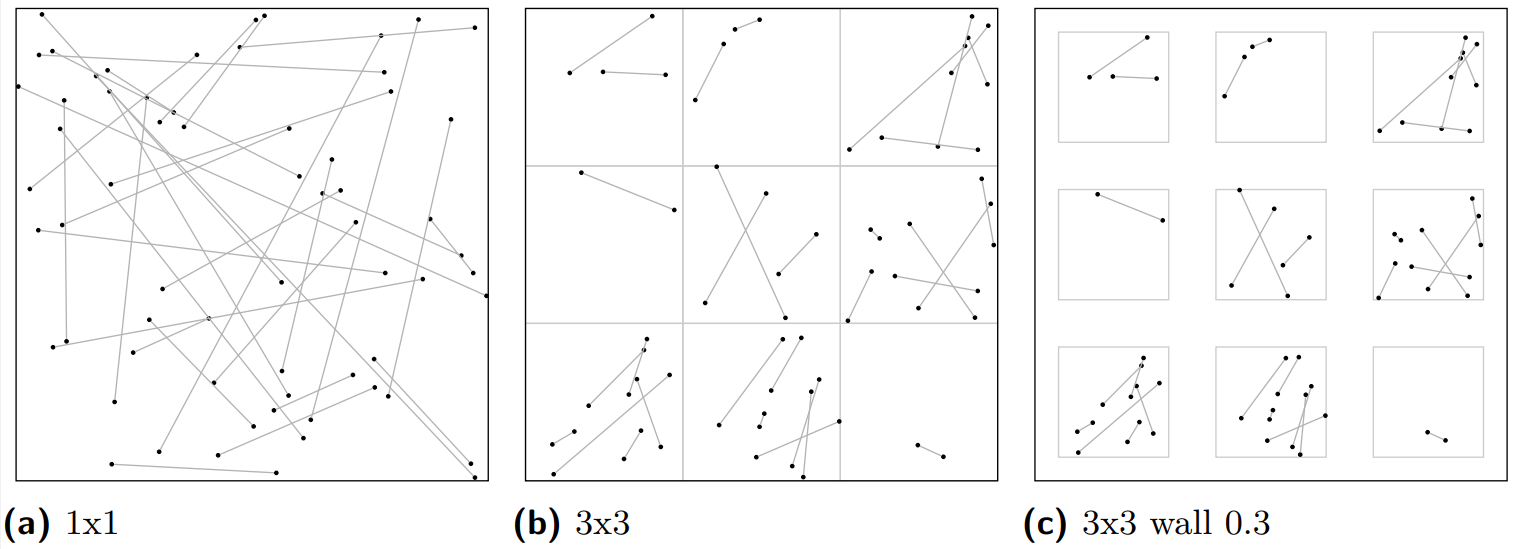
\includegraphics[scale=0.5]{imgs/instances_type_2.png}
    \caption{Instances randomly generated with 16 agents, in (a) a 1 x 1 frame with no wall, in (b) a 3 x 3 frame with \(0\%\) wall, and in (c) a 3 x 3 frame with \(30\%\) wall.}
    \label{fig:instances_type_2}
\end{figure}

\section{Computational Results}

A summary of the experiment results broken by instance group can be seen in Table~\ref{table_avg_apx}. The table shows the gap between the result achieved by the 3-approximation and the linear relaxation, as well as its respective execution times. The first line of the table shows the average results from the type 1 instances. The remaining table sub-divides the type 2 instances depending on some properties. The ``\(1 \times 1\)'' class contains results with a single frame, while the ``\(2 \times 2\)'' class contains the results of the instances with 4 frames, etc. The ``\(W0.x\)'' class contains the results of the instances with wall separation of \((10 \times x)\%\) of the size of the frame (as illustrated in the Figure~\ref{fig:instances_type_2} (c)). The last lines of the table separate the instances by the number of ``agents'' (which is how \citeauthor{Pereira2018TheSM} call terminal pairs).

\begin{table}[H]
\caption{Summary of results by class.}
\centering
    \begin{tabular}{lrrrr}
        \toprule
        Classes & num Inst & GAP (\%) & APX time (s) & relaxed solver time (s) \\
        \midrule
        m-PDTSP & 210 & 33.80 & 0.00 & 0.00 \\
        \hline
        1 $\times$ 1 & 15 & 41.06 & 159.34 & 0.09 \\
        2 $\times$ 2 & 75 & 40.67 & 46.45 & 0.09 \\
        3 $\times$ 3 & 75 & 36.46 & 45.01 & 0.10 \\
        4 $\times$ 4 & 75 & 32.89 & 64.33 & 0.09 \\
        5 $\times$ 5 & 75 & 30.77 & 100.85 & 0.09 \\
        \hline
        W0.0 & 75 & 36.90 & 145.25 & 0.09 \\
        W0.1 & 60 & 37.78 & 109.89 & 0.09 \\
        W0.2 & 60 & 35.36 & 55.96 & 0.09 \\
        W0.3 & 60 & 33.09 & 7.33 & 0.09 \\
        W0.4 & 60 & 32.72 & 5.91 & 0.09 \\
        \hline
        rg-016 & 63 & 23.76 & 0.00 & 0.00 \\
        rg-032 & 63 & 26.02 & 0.03 & 0.00 \\
        rg-064 & 63 & 34.63 & 0.56 & 0.02 \\
        rg-128 & 63 & 36.74 & 12.44 & 0.08 \\
        rg-256 & 63 & 40.98 & 330.44 & 0.35 \\
        \hline
        total average & & 34.21 & 197.10  & 0.29 \\
        \bottomrule
    \end{tabular}
\label{table_avg_apx}
\end{table}


We can see a positive trend between the number of agents (i.e., terminal pairs) and the solution gap. It is also possible to observe a negative trend between the number of frames and the quality of the solution, indicating that the algorithm does not handle well terminal pairs whose terminals are far from each other.

The relationship between the number of terminals in each instance and the optimality gap of the algorithm can be seen in Figure~\ref{fig:hist_opt_gap}. The figure shows that for all instances, the algorithm got significantly closer to the optimality than its 3-approximation guarantee. Although the results, accounting for both execution time and solution quality, were inferior to the heuristic proposed by \cite{Pereira2018TheSM}. 

% \begin{figure}[t!]
%     \centering
%     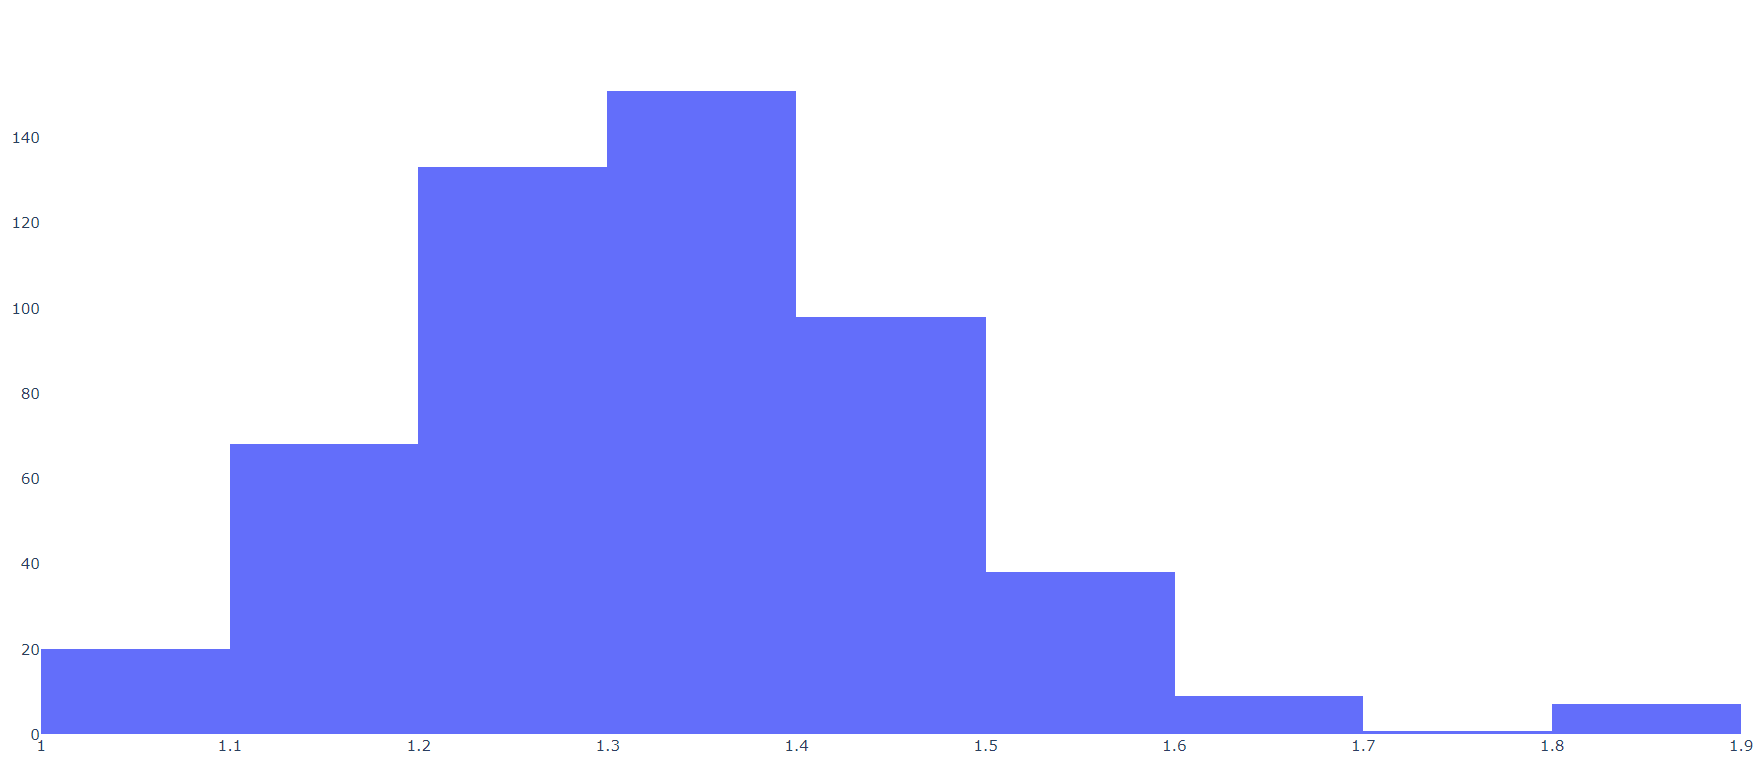
\includegraphics[scale=0.4]{imgs/hist_opt_gap2.png}
%     \caption{Number of instances per optimality gap. An optimality gap of \(1.6\) means that the solution cost is \(60\%\) more than the cost of the relaxation.}
%     \label{fig:hist_opt_gap}
% \end{figure}

\begin{figure}[t!]
\centering
\begin{tikzpicture}
\begin{axis}[
    ymin=0, ymax=80,
    minor y tick num = 3,
    area style,
    ]
\addplot+[ybar interval,mark=no] plot coordinates { (1.0476854749768996, 11) (1.0853661041789102, 14) (1.123046733380921, 33) (1.1607273625829317, 30) (1.1984079917849424, 52) (1.2360886209869533, 55) (1.273769250188964, 36) (1.3114498793909748, 63) (1.3491305085929854, 60) (1.386811137794996, 43) (1.424491766997007, 37) (1.4621723961990176, 36) (1.4998530254010283, 11) (1.5375336546030391, 7) (1.5752142838050498, 21) (1.6128949130070604, 1) (1.6505755422090713, 7) (1.688256171411082, 1) (1.7259368006130926, 0) (1.7636174298151035, 7) };
\end{axis}
\end{tikzpicture}
\caption{Number of instances per optimality gap. An optimality gap of \(1.6\) means that the solution cost is \(60\%\) more than the cost of the relaxation.}
\label{fig:hist_opt_gap}
\end{figure}

Although the algorithm tended to perform better on smaller instances, from the 10 worst performance instances (that is, with the largest gap from the linear relaxation), 9 are from the instances of type 1 containing only 6 terminal pairs.

The implementation of the 3-approximation algorithm executes the shortcut step in line~\eqref{alg:3-apx:shortcutting} by naively finding any Euclidean subgraph contained in each component of the solution; we conjecture that the quality of this algorithm could be improved by applying a more robust shortcutting strategy on the cost of a greater execution time.

In all instances, the time spent to calculate the 2-approximation for the Survivable Network Design Problem accounted for more than \(99\%\) of the total execution time of the algorithm. Moreover, the iterative calculation of Gomory-Hu trees, a step during the solving of the SNDP, has a significant impact on the total execution time, especially for bigger instances, as we can see in Table~\ref{table_gomory_hu_gap}.

\begin{table}[t!]
\caption{Participation of Gomory-Hu trees calculation on total execution time}
\label{table_gomory_hu_gap}
\centering
    \begin{tabular}{lrrrr}
        \toprule
        num vert & num inst & min (\%) & mean (\%) & max (\%) \\
        \midrule
        12 & 70 & 0.00 & 0.00 & 0.00 \\
        22 & 70 & 0.00 & 0.00 & 0.00 \\
        32 & 133 & 0.00 & 0.00 & 0.00 \\
        64 & 63 & 0.00 & 13.63 & 40.90 \\
        128 & 63 & 23.31 & 39.64 & 75.80 \\
        256 & 63 & 30.30 & 51.86 & 78.43 \\
        512 & 63 & 38.68 & 64.89 & 91.76 \\
        \bottomrule
    \end{tabular}
\end{table}

This step might be a good area to improve upon so that the algorithm presents a better execution time in bigger instances.

For practical implementations, a possible alternative would be to use faster heuristics instead of the 2-approximation for the SNDP step (see~\cite{Ker2005}). 
Such heuristics could greatly improve the performance of the algorithm, despite loosing theoretical guarantees of the quality of the solutions.

\chapter{PTAS for Graphs of Bounded Treewidth}
\label{chapter:ptas_bounded_tree}

\section{Algorithm Overview}

The algorithm receives as input a graph \(G_{in}\) with bounded treewidth, and a set \(\mathcal{D} = \{T_1, \dots, T_k\}\) of terminal pairs. It begins by defining a polinomial sized subset of all possible solutions. We provide a proof that this subset contains a solution not greater than a constant times \(\opt\). The algorithm then calculates the smallest solution, via a dynamic programming approach, that is contained on this subset and outputs it as result.

\section{Groups}

Given a set of vertices \(X\), a set of vertices \(S\) (a.k.a. central vertices) such that \(S \subseteq X\), and a number \(r\), we define a group \(\mathcal{G}_G(X, S, r)\), for some graph \(G\), as the union of \(S\) and those vertices of \(X\) that are at a distance in \(G\) of at most \(r\) from some vertex in \(S\).

Lemma~\ref{groupLemma} presented below, states that the distance between any vertex of \(X\) and some vertex of \(S\) is at most \(\epsilon W\).

\begin{flemma} \label{groupLemma}
Let \(C\) be a cycle that contains the terminals \(X \subseteq V(G)\) and has cost \(W\). For all \(0 < \epsilon < 1\), there is a set \(S \subseteq X\) of \(\mathcal{O}(1 + 1/\epsilon)\) vertices such that \(X = \mathcal{G}_G(X, S, \epsilon W)\).
\end{flemma}
\begin{proof}

We construct \(S\) iteratively as follows. 
First, we choose any vertex in \(X\) and add it to \(S\). Then we add the maximum number of vertices from \(X\) into \(S\) such that the distance between \(s_i\) and \(s_j\) for \(j \in \{1, \dots, i-1\}\) is at least \((\epsilon W)/2\), where $s_i$ and $s_j$ are the $i$-th and $j$-th vertices added to $S$. Let \(s_t\) be the last vertex added to \(S\). Note that, in case \(t = 1\), that is \(s_1\) is the only vertex added to \(S\), all the vertices of \(X\) are within a maximum distance of \((t \epsilon W)/2\) from vertex \(s_1\), thus the result holds.

Considering that \(t > 1\), the shortest closed walk between the vertices in \(S = \{s_1, \dots, s_t\}\), not necessarily in order, has a cost of at least \((t \epsilon W)/2\). Thus \(t \leq 2/\epsilon\) is valid. So we conclude that all vertices of \(X\) are at distance at most \(\epsilon W\) from \(S = \{s_1, \dots, s_t\}\) with \(t = 2/\epsilon\).
\end{proof}

\begin{fcorollary} \label{groupCor}
If \(S_1\), \(S_2\), \(X_1\), \(X_2\) are subsets of \(V(G)\) and \(r_1, r_2 \in \mathbb{R}\), then \[\mathcal{G}_G(X_1, S_1, r_1) \cup \mathcal{G}_G(X_2, S_2, r_2) \subseteq \mathcal{G}_G(X_1 \cup X_2, S_1 \cup S_2, \max\{r_1, r_2\})\]
\end{fcorollary}
\begin{proof}

Let \(v \in \mathcal{G}_G(X_i, S_i, r_i)\) with $i \in \{1,2\}$. The result is valid if \(v \in S_i\). Suppose \(v \in X_i\), but \(v \not\in S_i\). Note that \(v \in X_1 \cup X_2\), and there is \(x \in S_i\) such that the distance between \(v\) and \(x\) in \(G\) is at most \(r_i\). Therefore, \(v\) belongs to \(\mathcal{G}_G(X_1 \cup X_2, S_1 \cup S_2, \max\{r_1, r_2\})\).

\end{proof}

\section{Notation and definitions}

Let  \((T, \mathcal{B})\) denote a nice tree decomposition of \(G\) with treewidth \(\kappa\). Let \(I\) be the set of nodes of \(T\), and let \(\mathcal{B} = \{B_i \colon i \in I\}\) be the set of bags of the decomposition.

For a given bag \(B_i\), we denote by \(V_i\) the set of vertices that belongs to \(B_i\) or any of its descendants in \(T\). We denote as \textbf{active} in \(B_i\) the set of terminals \(A_i \subseteq V_i\) such that for each \(t \in A_i\) there is a terminal pair \(\{t, t'\} \in \mathcal{D}\) with \(t' \in V(G)\backslash V_i\).

Let \(G_i = G[V_i]\) and let \(M_i\) be a subgraph of \(G_i\) that contains \(A_i\). We denote as \(\pi_i(M_i)\) the partition of \(A_i\) induced by the components of \(M_i\).

A partition \(\alpha\) of a set \(S\) can be considered an equivalence relation on \(S\). We use \((x, y) \in \alpha\) to indicate that \(x\) and \(y\) are in the same class of \(\alpha\), and \(x^\alpha\) denotes the class of \(\alpha\) that contains the element \(x\).

If \(M\) is a subgraph of \(G\) and \(S \subseteq V(G)\), then \(M\) induces a partition \(\alpha\) of \(S\), where \((x, y) \in \alpha\) if and only if \(x\) and \(y\) are in the same component of \(M\) (and every \(x \in S \backslash V(M)\) forms its own class, so \(M\) does not have to be a spanning subgraph). We say that a partition \(\alpha\) is \textbf{finer} than a partition \(\beta\) if \((x, y) \in \alpha\) implies \((x, y) \in \beta\); in that case we say that \(\beta\) is \textbf{coarser} than \(\alpha\). We denote as \(\alpha_1 \vee \alpha_2\) the finest partition which is coarser than both \(\alpha_1\) and \(\alpha_2\).

Let \(\beta_i\) be a partition of \(B_i\) for some \(i \in I\) and let \(M_i\) be a subgraph of \(G_i\). We denote as \(M_i + \beta_i\) the graph obtained from $M_i$ by adding a new edge \(xy\) for each \((x, y)\) vertex pair that is in the same class in \(\beta_i\). Note that \(M_i + \beta_i\) is not necessarily a subgraph of \(G_i\).

We define the \textbf{top bag} of a vertex \(v\) as the bag that contains \(v\) and is the closest in $T$ to the root.
Given two vertices \(u\) and \(v\), we say that \(u < v\) when the top bag of \(u\) is a descendent of the top bag of \(v\). Note that in a nice tree decomposition, each bag is the top for at most one vertex since a forget node can lose only one vertex when compared to its descendent node. Also note that if there is at least one bag that contains both \(u\) and \(v\), then either \(u < v\) or \(v < u\) is valid.

Let \(K_i\), for \(i \in \{1, 2\}\), be a set of vertices that induces a connected component in \(G\). Also consider that \(K_1\) and \(K_2\) are disjoint. We extend the previous concept so that \(K_1 < K_2\) if there is a vertex \(v\) in \(K_2\) such that \(u < v\) for all vertices \(u \in K_1\). Recall from the definition of the nice tree decomposition, that for a given bag, at most one vertex can be forgotten; considering that, there is always a vertex \(v \in K_1 \cup K_2\) such that all vertices in \(K_1 \cup K_2 \backslash \{v\}\) are decedents from.

As a consequence of the construction of the nice tree decomposition, if there is a bag containing vertices of both \(K_1\) and \(K_2\), then \(K_1 < K_2\) or \(K_2 < K_1\) is valid.

Finally, the following lemma from \cite{Bateni} guarantees some properties we shall use in our dynamic programming algorithm.

\begin{flemma}[\cite{Bateni} Lemma 2.1]\label{bateni_2_1}
Let \(G\) be a graph having no connected component consisting of a single edge. \(G\) has a nice tree decomposition of polynomial size with the following two additional properties:

\begin{enumerate}
    \item No introduce node introduces a degree 1 vertex.
    \item The vertices in a join node have a degree greater than 1.
\end{enumerate}

\end{flemma}

\section{Constructing the Partitions}

Let \(\Pi_i\) be a set of partitions of the active vertices \(A_i\), where $i \in I$.
Let \(\Pi = \{\Pi_i\}_{i \in I}\) be a collection of such partitions.

If some collection \(M\) of cycles satisfy \(\pi_i(M) \in \Pi_i\) for every \(i \in I\) (i.e., the partition of \(A_i\) induced by \(M\) belongs to \(\Pi_i\)), then we say that \(M\) \textbf{conforms} to \(\Pi\). This chapter aims to give an algorithm for bounded treewidth graphs that finds a minimum-cost solution conforming to a certain \(\Pi\) that we will build.

\begin{figure}[H]
    \centering
\begin{tikzpicture}

\draw (2,2) ellipse (4.5cm and 1.5cm) node at (-2.6,3) {$B_i$};

\draw (0,-2) -- (0,-1);
\draw (2,-2) -- (2,-1);
\draw [double distance=1pt](4,-2) -- (4,-1);

\draw [dotted](0,-1) -- (0,0);
\draw [dotted](2,-1) -- (2,0);
\draw [dotted](4,-1) -- (4,0);

\draw (0,0) -- (0,2);
\draw (2,0) -- (1.5,2);
\draw [double distance=1pt](4,0) -- (4.5,2);

\draw (0,2) -- (0,4);
\draw (1.5,2) -- (1.5,4);
\draw [double distance=1pt](4.5,2) -- (4.5,4);

\draw [dotted](0,4) -- (0,5);
\draw [dotted](1.5,4) -- (1.5,5);
\draw [dotted](4.5,4) -- (4.5,5);

\Vertex[x=0.0,y=2]{A}
\Vertex[x=1.5,y=2]{B}
\Vertex[x=3.0,y=2]{C}
\Vertex[x=4.5,y=2]{D}


\Vertex[x=0.0,y=-2,Math,IdAsLabel]{{A_i}_1}
\Vertex[x=2.0,y=-2,Math,IdAsLabel]{{A_i}_2}
\Vertex[x=4.0,y=-2,Math,IdAsLabel]{{A_i}_3}

\Edge[lw=0.7pt]({A_i}_1)({A_i}_2)

\end{tikzpicture}
    \caption{View of solution \(M\) on bag \(B_i\). This solution induces a partition \(\pi_i(M) = \{\{{A_i}_1, {A_i}_2\}, \{{A_i}_3\}\}\) of \(A_i\). If this partition belongs to \(\Pi_i\), then \(M\) conforms to \(\Pi_i\).}
    \label{fig:example_Ai_partition}
\end{figure}

In order to build \(\Pi_i\), consider \(j \in \{1, \dots, \kappa + 1\}\), where \(\kappa\) is the treewidth of~\(G\). 

Let \(S_j\) be a set of vertices of \(G_i\) with size \(\mathcal{O}((\kappa + 1)(1 + 1/\epsilon))\). Let \(r_j\) be a nonnegative real number equal to the distance between any two vertices in \(G\). Think of it as fetching two random vertices from \(G\) and assigning the distance between them to \(r_j\).

Each partition \(\pi\) of \(\Pi_i\) is built from a sequence \(S = ((S_1, r_1), \dots, (S_p, r_p))\) of \(p \le \kappa + 1\) pairs and a partition \(\rho\) of \(\{1, \dots, p\}\).

We build the partition \(\pi\) in the following way. Each pair \((S_j, r_j)\) defines a group \(R_j = \mathcal{G}_G(A_i, S_j, r_j)\) of \(A_i\) where \(i\in I\). In order to ensure that the classes of \(\pi\) are disjoint, we define \(R'_k := R_k \backslash \bigcup^{k-1}_{l=1} R_l\) for each $k \in \{1, \ldots p\}$.

For each class \(P \in \rho\), there is a class in \(\pi\) which corresponds to the union of~\(R'_j\) for \(j \in P\). Precisely, for each \(P \in \rho\),  let \(\bigcup_{j \in P} R'_j\) be a class of \(\pi\). If \(\pi\) covers all vertices in \(A_i\), then we put the resulting partition of \(A_i\) induced by \(\pi\) into \(\Pi_i\); otherwise, we ignore \(\pi\). This process is repeated considering all possible sequences \(S\) and all partitions \(\rho\) of the sequence's elements.

To show that this process is indeed polynomial, let \(n = |V(G)|\) and \(y = \mathcal{O}((\kappa + 1)(1 + 1/\epsilon))\). There are \(n \choose y \) \(\leq n^y\) possible sets \(S_j\) and, by consequence, \(n^y \cdot n^2\) pairs \((S_j, r_j)\). With that, there are \(n^{y + \kappa + 1} \cdot n^2\) possible sequences of size \(\kappa + 1\) created by pairs \((S_j, r_j)\) and partitioned by \(\rho\). Since we consider all those sequences in order to build \(\Pi_i\), the size of \(\Pi_i\) is polynomial in \(|V(G)|\) considering \(\kappa\) and \(\epsilon\) constants.

\begin{ftheo}\label{conformingPi}

There is a solution to the SMCP that conforms to \(\Pi\) on graphs of treewidth \(\kappa\) whose cost is no greater than \((1 + 2 \kappa \epsilon)\) times the minimum cost.

\end{ftheo}
\begin{proof}

Let \(G\) be a graph with treewidth \(\kappa - 1\), let \(\mathcal{D}\) be a set of terminal pairs \(\{\{t_1, t_1')\}, \dots, \{t_k, t_k'\}\}\), and  let \(\epsilon > 0\) be a constant.
Let \(M^\ast\) be a minimum-cost collection of cycles concerning \(G\) and \(\mathcal{D}\).

We will describe a procedure to add edges to \(M^\ast\) in such a way that the resulting collection of cycles \(M\) conforms to \(\Pi\) and has a maximum size of \((1 + 2\kappa \epsilon ) \cdot c(M^\ast)\).

Let \(H^\ast\) be the subgraph of \(G\) induced by the edges in \(M^\ast\). Let \(H\) be the equivalent to \(M\). Note that, since \(H\) is composed of \(H^\ast\) plus some additional edges, \(H\) is a super graph of \(H^\ast\), and the components of \(H\) define a partition of the components of \(H^\ast\).

Initially we set \(H = H^\ast\). Suppose there is a bag \(B_i\) whose partition \(\pi_i(H)\) of \(A_i\) is not in \(\Pi_i\). Let \(K_1 < K_2 < \dots < K_p\) be the components of \(H^\ast\) that intersects \(B_i\), ordered by the relation \(<\) (which was presented above). Let \(\rho\) be the partition of \(\{1, \dots, p\}\) (which corresponds to the components of \(H^\ast\) that intersects \(B_i\)) induced by the components of \(H\).

Let \(A_{i, j}\) be the subset of \(A_i\) connected by \(K_j\). By Lemma~\ref{groupLemma} and Corollary~\ref{groupCor} there is a set \(S_j \subseteq K_j\) of at most \(O(1 + 1/\epsilon)\) vertices of \(K_j\) such that \(A_{i,j} = \mathcal{G}_G(A_{i,j}, S_j, r_j)\), for some \(r_j \leq c(K_j)\).

Let \(\pi\) be a partition generated from the sequence \(((S_1, r_1), \dots, (S_p, r_p))\) and the partition \(\rho\), as described before. Suppose that \(\pi \notin \Pi_i\).

Let \(R_j\) and \(R'_j\) as defined in \(\Pi_i\) construction (i.e., \(R_j = \mathcal{G}_G(A_i, S_j, r_j)\)). Let \(\rho(j)\) be the class of \(\rho\) that contains \(j\). If for all \(1 \leq j \leq p\)  the vertices of \(A_{i,j}\) are contained in \(\bigcup_{j' \in \rho(j)}R'_{j'}\) then \(\pi \in \Pi_i\).
Thus there is a vertex \(v \in A_{i,j}\) which is not in \(\bigcup_{j' \in \rho(j)}R'_{j'}\). As \(v \in R_j\) (since \(A_{i,j} \in R_j\)) then \(v \in R_{j^\ast}\) also hold for some \(K_{j^\ast} < K_j\) and \(j^\ast \not\in \rho(j)\).

The fact that \(R_{j^\ast} = \mathcal{G}_G(A_i, S_{j^\ast}, r_{j^\ast})\) contains \(v \in A_{i, j}\) means that there is a vertex \(u \in S_{j^\ast}\) such that \(dist_{G_i}(u, v) \leq r_{j^\ast} \leq \epsilon c(K_{j^\ast})\). We add to \(H\) a shortest path in \(G\) connecting \(u\) and \(v\). That increases the size of \(M\) in at most \(2 \epsilon c(K_{j^\ast})\), since each edge of the path may be covered twice, so it guarantees a cycle. This implies that the increased size of \(H\) is at most \(\epsilon c(K_{j^\ast})\).


\begin{figure}[H]
    \centering
\begin{tikzpicture}

\draw (2,2) ellipse (4.5cm and 1.5cm) node at (-2.6,3) {$B_{i-1}$};

\draw (2,-2) ellipse (4.5cm and 1.5cm) node at (-2.6,-1) {$B_i$};

\draw[red,thick,dashed] (1,-5) arc(0:180:1cm and 4cm) node at (-1,-1.5) {$K_{j^\ast}$};

\draw[red,thick,dashed] (1.3,-5) .. controls (0.7,0.0) .. (1.3,4) node at (0.8,3.8) {$K_j$};

\draw[red,thick,dashed] (3.2,-5) .. controls (3.8,0.0) .. (3.2,4);


\Vertex[x=1.5,y=2, label=B]{B}
\Vertex[x=3.0,y=2, label=C]{C}
\Vertex[x=4.5,y=2, label=D]{D}

\Vertex[x=0.0,y=-2, label=A]{Ai}
\Vertex[x=1.5,y=-2, label=B]{Bi}
\Vertex[x=3.0,y=-2, label=C]{Ci}
\Vertex[x=4.5,y=-2, label=D]{Di}

\Vertex[x=0.0,y=-4.3]{V1}
\Vertex[x=2.25,y=-4.3]{V2}

\Edge[color=red, lw=3pt](V1)(V2)

\end{tikzpicture}
    \caption{Example of connection between \(K_{j^\ast}\) and \(K_j\). Note that \(K_{j^\ast} < K_j\). The thick red line represents the connection created between both components. This connection consists of the shortest path between both components (it does not necessarily go through edges in \(B_i\)).}
    \label{fig:connect_k_j_ast_and_k_j}
\end{figure}


This increase is due the pair \((K_{j^\ast}, K_j)\). Notice that this pair of components of \(H^\ast\) are now part of the same component of \(H\) and will not be connected again. This process is illustrated in Figure~\ref{fig:connect_k_j_ast_and_k_j}.

Note that we are charging only to pairs \((K, K')\) having the property that \(K < K'\), and there is a bag containing vertices from both \(K\) and \(K'\). Observe that if \(B_i\) is the topmost bag where vertices from \(K\) appear, then these properties imply that a vertex of \(K'\) appears in this bag as well. Thus a component \(K\) can be the first component of at most \(\kappa\) such pairs \((K, K')\): since the components are disjoint, the topmost bag containing vertices from \(K\) can intersect at most \(\kappa\) other components. We will charge a cost increase of at most \(2 \epsilon \cdot c(K)\) on the pair \((K, K')\), thus the total increase is at most \(2\kappa\epsilon \cdot c(M^\ast)\).

Since the modification always extends \(H\), the procedure terminates after a finite number of steps. By the end of this process, each partition \(\pi_i(M)\) belongs to the corresponding \(\Pi_i\), thus the solution \(M\) conforms to \(\Pi\) and its cost is at most \((1 + 2\kappa\epsilon) \cdot c(M^\ast)\).
\end{proof}

\section{Conforming Solutions}

The primary strategy during the dynamic programming is to use Theorem~\ref{conformingPi} to bound the number of subsolutions we need to evaluate at each bag of the decomposition.

The proof is based on a standard dynamic programming approach. Initially, we perform the following simple transformation on the graph to make the process easier. 
For each terminal \(v\) of \(G\), we create a vertex \(v'\) and a zero-weight edge between \(v\) and \(v'\), then we replace \(v\) by \(v'\) as the new terminal. Notice that, after this transformation, all terminals have degree 1, and the size of the minimum Steiner Multicycle stays unchanged.

One well-known fact is that any tree decomposition can be converted into a \(\emph{nice}\) tree decomposition of the same width within polynomial time (\cite{CyganBook}, Lemma~7.4). 

Consider a nice tree decomposition $(T, \mathcal{B})$ of $G$. In this decomposition, all terminals are located at leaf nodes, ensuring that join nodes, as per Lemma~\ref{bateni_2_1}, do not introduce any new terminals.

For the dynamic programming, we define a sub-problem for each node \(i \in I\). The idea is that the solution of a sub-problem \(i\) generates a multiset \(M_i\) of edges of \(G_i\) in such a way that \(M_i\) is equal to the final solution \(M\) restricted to \(G_i\).

For simplicity, throughout the proof, we can also observe an edges multiset \(M\) as the subgraph induced by its edges. That way, we can talk about components of \(M\), i.e., the components of the subgraph of $G$ induced by the edges in \(M\). Note, however, that \(c(M)\) is the sum of the cost of all the edges in the multiset \(M\), considering repetitions.

Due to the possibility that two components of \(M_i\) belong to the same component in \(M\), the components of \(M\) partition \(A_i\) in a coarser way than \(M_i\). Consequently, requiring that \(\pi_i(M_i) \in \Pi_i\) during the process is not feasible. To address this issue, we introduce a partition \(\beta_i\) of \(B_i\) that captures the partition of the components of \(M_i\) induced by the final solution \(M\). Since we do not know \(M\) during the process, for each bag \(B_i\), we create a set of solutions considering \(\beta\) as all the possible combinations of the partitions of \(B_i\) induced by \(M_i\). Notice that, for each bag \(B_i\), the number of possible combinations of \(\beta_i\) is at most the \(\kappa\)-th Bell number (which can be calculated as \(B_{\kappa} = \sum_{i=0}^{\kappa - 1} \binom{\kappa - 1}{i} B_{\kappa - 1}\)), thus a constant number of combinations, considering \(\kappa\) fixed.

Formally, each solution \(c = (i, H, \pi, \alpha, \beta, \mu)\) of a subproblem should respect

\begin{itemize}
    \item[(S1)] \(i \in I\) is a node of \(T\);
    \item[(S2)] \(H\) is a multiset of edges that induces a spanning subgraph of \(G[B_i]\) (i.e., contains all vertices of \(G[B_i]\)), in such a way that edges can be crossed multiple times;
    \item[(S3)] \(\pi \in \Pi_i\) is a partition of \(A_i\);
    \item[(S4)] \(\pi\), \(\beta\) are partitions of \(B_i\), \(\beta\) is coarser than \(\alpha\), and \(\alpha\) is coarser than the partition induced by the components of \(H\);
    \item[(S5)] \(\mu\) is a injective mapping from the classes of \(\pi\) to the classes of \(\beta\).
\end{itemize}

The item (S5) of the subproblem maps which vertices of \(B_i\) belong to the component connected to some vertex of \(A_i\) to guarantee that no vertex of \(A_i\) becomes ``lost'' and does not connect to its pair.

A solution \(c = (i, H, \pi, \alpha, \beta, \mu)\) of a subproblem is the minimum cost of a multiset \(M_i\) with edges of \(G[V_i]\), satisfying all of the following requirements:

\begin{itemize}
    \item[(C1)] \(M_i[B_i] = H\) (which implies \(B_i \subseteq V(M_i)\));
    \item[(C2)] \(\alpha\) is the partition of \(B_i\) induced by \(M_i\);
    \item[(C3)] \(\pi\) is the partition of \(A_i\) induced by \(M_i + \beta\);
    \item[(C4)] For each descendent \(d\) of \(i\), (including \(d = i\)) the partition of \(A_d\) induced by \(M_i + \beta\) belongs to \(\Pi_d\);
    \item[(C5)] If there is a terminal pair \((x_1, x_2)\), with \(x_1, x_2 \in V_i\), then they are connected in \(M_i + \beta\);
    \item[(C6)] Every \(x \in A_i\) is in the component of \(M_i + \beta\) containing \(\mu(x^\pi)\).
    \item[(C7)] Every vertex \(v \in M_i\) must have an even degree (accounting for edges duplicity).
\end{itemize}

With that at hand, we proceed to the main result of this chapter.

\begin{ftheo}\label{dynamicProgramming}

Let \(G\) be a graph with treewidth bounded by \(\kappa\). Let \(\epsilon > 0\) be a constant. Let \(\mathcal{D}\) be a set of terminal pairs. Let \(\Pi\) be a set of partitions of vertices of \(G\), built as described above.
There exists a polynomial-time algorithm to find a multiset of edges \(M\) (i.e., a collection of cycles), satisfying the following properties:
\begin{enumerate}
    \item Every vertex \(v \in G\) is an endpoint of an even number of edges in \(M\).
    \item The subgraph induced by \(M\) connects all the terminal pairs of \(\mathcal{D}\).
    \item \(M\) conforms to \(\Pi\).
    \item \(c(M) \leq (1 + 2 \kappa \epsilon) \opt\).
\end{enumerate}

\end{ftheo}
\begin{proof}


We solve the previously described subproblems by bottom-up dynamic programming, considering each node $i \in I$. We perform different processes for each node type, as detailed below.


\noindent {\large Leaf Node \(i\)}.

If \(i\) is a leaf node, the solution's value is trivially 0.

\noindent {\large Join Node \(i\) with children \(i_1\) and \(i_2\)}.

% TODO colocar claims em um ambiente minipage

\begin{claim} \label{sub_solution_join}
    Let $i \in I$ be a join node with children $i_1$ and $i_2$.
    So, \(A_{i_1}\) and \(A_{i_2}\) are disjoint and \(A_i\) is a subset of the union of \(A_{i_1} \cup A_{i_2}\).
    The value of the subproblem $(i, H, \pi, \alpha, \beta, \mu)$ is:
\begin{align*}
  c(i, H, \pi, \alpha, \beta, \mu) = \min_{(J1), (J2), (J3), (J4)} \left(c(i_1, H, \pi^1, \alpha^1, \beta, \mu^1) + c(i_2, H, \pi^2, \alpha^2, \beta, \mu^2) - c(H)\right)
\end{align*}

where the minimum is taken over all tuples satisfying the following properties:

\begin{enumerate}[(J1)]
    \item \(\alpha^1 \vee \alpha^2 = \alpha\);
    \item \(\pi\) and \(\pi^p\) are the same on \(A_{i_p} \cap A_i\), for each \(p  \in \{1, 2\}\);
    \item For every \(p  \in \{1, 2\}\) and \(v \in A_i \cap A_{i_p}\), \(\mu(v^\pi) = \mu^p(v^{\pi^p})\); and
    \item If there is a terminal pair \((x_1, x_2)\) with \(x_1 \in A_1\) and \(x_2 \in A_2\) then \(\mu^1(x_1^{\pi^1}) = \mu^2(x_2^{\pi^2})\), in other words, both terminals must be mapped to the same partition of \(\beta\).
\end{enumerate}

\end{claim}

\begin{proof}
Let \(Q_1 = (i^1, H, \pi^1, \alpha^1, \beta, \mu^1)\) and \(Q_2 = (i^2, H, \pi^2, \alpha^2, \beta, \mu^2)\) be subproblems minimizing the right-hand side of (8), and let \(M_1\) and \(M_2\) be optimal solutions of \(Q_1\) and \(Q_2\), respectively. Let \(M_i\) be the union of subgraphs \(M_1\) and \(M_2\). It is clear that the cost of \(M_i\) is exactly the right-hand side of the equation in Claim~\ref{sub_solution_join} since the common edges of \(M_1\) and \(M_2\) are exactly the edges of \(H\).

We next show that \(M_i\) is a solution of \(P_i\), that is, \(M_i\) satisfies properties (C1)–(C7).

\begin{itemize}
    \item[(C1)] Follows from \(M_1[B_i] = M_2[B_i] = M_i[B_i] = H\).
    \item[(C2)] Follows from (J1) and from the fact that \(M_1\) and \(M_2\) intersect only in \(B_i\).
    \item[(C3)] First consider two vertices \(x, y \in A_i^p \cap A_i\). Vertices \(x\) and \(y\) are connected in \(M_i + \beta\) if and only if they are connected in \(M_p + \beta\). By (C3) for \(M_p\), this is equivalent to \((x, y) \in \pi_p\), which is further equivalent to \((x, y) \in \pi\) by (J2). Now suppose that \(x \in A_i^1 \cap A_i\) and \(y \in A_i^2 \cap A_i\). In this case, \(x\) and \(y\) are connected in \(M_i + \beta\) if and only if there is a vertex of \(B_i\) reachable from \(x\) in \(M_1 + \beta\) and from y in \(M_2 + \beta\), or in other words, \(\mu_1(x^\pi_1) = \mu_2(x^\pi_2)\). By (J3), this is equivalent to \(\mu(x^\pi) = \mu(y^\pi)\), or \((x, y) \in \pi\) (as \(\mu\) is injective).
    \item[(C4)] If \(d\) is a descendant of \(i_p\) with $p \in \{1,2\}$, then the statement follows using that (C4) holds for solution \(M_p\) of \(P_p\) and the fact that for every descendant \(d\) of \(i_p\), \(M_p + \beta\) and \(M_i + \beta\) induce the same partition of \(A_d\). For \(d = i\), the statement follows from the previous paragraph, that is, from the fact that \(M_i + \beta\) induces partition \(\pi \in \Pi_i\) of \(A_i\).
    \item[(C5)] Consider a pair \((x_1, x_2)\). If \(x_1, x_2 \in V_{i_p}\), then the statement follows from (C5) on \(M_p\). Suppose now that \(x_1 \in V_{i_1}\) and \(x_2 \in V_{i_2}\); in this case, we have \(x_1 \in A_{i_1}\) and \(x_2 \in A_{i_2}\). By (C6) on \(M_1\) and \(M_2\), \(x_p\) is connected to \(\mu^p(x_p^{\pi^p})\) in \(M_p + \beta\). By (J4), we have \(\mu^1(x_1^{\pi^1}) = \mu^2(x_2^{\pi^2})\), hence \(x_1\) and \(x_2\) are connected to the same class of \(\beta\) in \(M_i + \beta\).
    \item[(C6)] Consider an \(x \in A_i\) that is in \(A_{i_p}\). By condition (C6) on \(M_p\), we have that \(x\) is connected in \(M_p + \beta\) (and hence in \(M_i + \beta\)) to \(\mu^p(v^\pi_p)\), which equals \(\mu(v^\pi)\) by (J3).
    \item[(C7)] Also follows from \(M_1[B_i] = M_2[B_i] = M_i[B_i] = H\) since no edges were removed from or added to the children subproblems.
\end{itemize}

% prova volta

% Proof of left \(\geq\) right:
We now proceed to show the other inequality, that is, the left-hand side is at least the right-hand side.
Let \(M_i\) be a solution of subproblem \((i, H, \pi, \alpha, \beta, \mu)\) and let \(M_p\) be the subgraph of \(M_i\) induced by \(V_{i_p}\). To prove the inequality, we need to show three things. First, we have to define two tuples \((i_1, H, \pi^1, \alpha^1,\beta,\mu^1)\) and \((i_2, H, \pi^2, \alpha^2,\beta,\mu^2)\) that are subproblems, that is, they satisfy (S1)–(S5). Second, we need to show that (J1)–(J4) hold for these subproblems. Third, we need to show that \(M_1\) and \(M_2\) are solutions for these subproblems (i.e., respects (C1)–(C7)). Hence, they can give an upper bound on the right-hand side that matches the cost of \(M_i\).

Let \(\alpha^p\) be the partition of \(B_i\) induced by the components of \(M_p\); as \(M_1\) and \(M_2\) intersect only in \(B_i\), we have \(\alpha = \alpha^1 \vee \alpha^2\), ensuring (J1). Since \(\beta\) is coarser than \(\alpha\), it is coarser than both \(\alpha^1\) and \(\alpha^2\). Let \(\pi^p\) be the partition of \(A_{i_p}\) defined by \(M_i + \beta\); we have \(\pi^p \in \Pi_{i_p}\) by (C4) for \(M_i\). Furthermore, by (C3) for \(M_i\), \(\pi\) is the partition of \(A_i\) induced by \(M_i + \beta\), hence it is clear that \(\pi\) and \(\pi^p\) are the same on \(A_{i_p} \cap A_i\), so (J2) holds. This also means that \(M_i + \beta\) (or equivalently, \(M_p + \beta\)) connects a class of \(\pi^p\) to exactly one class of \(\beta\); let \(\mu^p\) be the corresponding mapping from the classes of \(\pi^p\) to \(\beta\). Now (J4) is immediate.

It is clear that the tuple \((i_p, H, \pi^p, \alpha^p, \beta, \mu^p)\) satisfies (S1)–(S5), since it is a subproblem. We need to show that \(M_p\) is a solution of the subproblem \((i_p, H, \pi^p, \alpha^p, \beta, \mu^p)\). As the edges of \(H\) are shared by \(M_1\), and \(M_2\), it will follow that the right-hand side is not greater than the left-hand side.

\begin{itemize}
    \item[(C1)] Obvious from the definition of \(M_1\) and \(M_2\).
    \item[(C2)] Follows from the definition of \(\alpha^p\).
    \item[(C3)] Follows from the definition of \(\pi^p\), and from the fact that \(M_i + \beta\) and \(M_p + \beta\) induce the same partition on \(A_{i_p}\).
    \item[(C4)] Follows from (C4) on \(M_i\) and from the fact that \(M_i + \beta\) and \(M_p + \beta\) induces the same partition on \(A_d\).
    \item[(C5)] Suppose that \(x_1, x_2 \in V_{i_p}\). Then, by (C5) for \(M_i\), \(x_1 \) and \(x_2\) are connected in \(M_i + \beta\).
    \item[(C6)] Follows from the definition of \(\mu^p\).
    \item[(C7)] Follows from \(M_1[B_i] = M_2[B_i] = M_i[B_i] = H\).
\end{itemize}
\end{proof}

\noindent {\large Introduction Node \(i\) of vertex \(v\)}.

\begin{claim}
Let \(j\) be the child of \(i\). Since \(v\) is not a terminal, \(A_i = A_j\). Let \(M'\) be a subgraph of \(G[V_j]\), let \(M_S\) be the subgraph obtained from \(M'\) by adding the vertex \(v\) to \(M'\), making \(v\) adjacent to \(S \subseteq B_j\). To guarantee (C7), we need to ensure that all vertices in \(v \cup S\) have even degree, so we get the connection of the least cost between \(v\) and each \(s \in S\) which guarantees such property.

Since \(|S| \leq \kappa\), this can be calculated in constant time. Let \(R\) be the multiset of added edges (possibly with repetition). Note that, for a given vertex \(s \in S\), the edge \(vs\) needs to be crossed at most twice for the solution to be valid.

If \(\alpha'\) is the partition of \(B_j\) induced by the components of \(M'\), then we define the partition \(\alpha' [v, S]\) of \(B_i\) to be the partition obtained by joining all classes of \(\alpha'\) that intersects S and adding \(v\) to this new class. It is clear that \(\alpha'[v, S]\) is the partition of \(B_i\) induced by \(M_S\).

The value of the subproblem is:

\begin{align*}
c(i, H, \pi, \alpha, \beta, \mu) = \min_{(I1), (I2), (I3)} c(j, H[B_j], \pi, \alpha', \beta', \mu') + \sum_{e \in R}c(e),
\end{align*}

Where the minimum is taken over all tuples satisfying the following conditions:

\begin{itemize}
    \item[(I1)] \(\alpha_i = \alpha_j[v, S]\) where \(S\) is the set of neighbors of \(v\) in \(H\);
    \item[(I2)] \(\beta'\) is \(\beta\) restricted to \(B_j\);
    \item[(I3)] For every \(x \in A_i\), \(\mu_i(x^\pi)\) is the class of \(\beta\) containing \(\mu'(x^\pi)\).
\end{itemize}

\end{claim}

\begin{proof}
Proof of left \(\leq\) right:
Let \(M'\) be an optimal solution of subproblem \(P' = (j , H[B_j], \pi, \alpha', \beta', \mu')\). Let \(M_i\) be the graph obtained from \(M'\) by adding to it the edges of \(H\) incident to \(v\); it is clear that the cost of \(M_i\) is exactly the right-hand side. Let us verify that (C1)–(C7) hold for \(M_i\).

\begin{itemize}
    \item[(C1)] Immediate.
    \item[(C2)] Holds because of (I1) and the way \(\alpha'[v, S]\) was defined.
    \item[(C3)–(C5)] Observe that \(M_i + \beta\) connects two vertices of \(V_j\) if and only if \(M' + \beta'\) does. Indeed, if a path in \(M_i + \beta\) connects two vertices via vertex \(v\), then the two neighbors \(x\), \(y\) of \(v\) on the path are in the same class of \(\beta\) as \(v\) (using that \(\alpha\) and \(\beta\) are coarser than the partition induced by \(H\)); hence, (I2) implies that \(x\), \(y\) are in the same class of \(\beta'\) as well. In particular, for every descendant \(d\) of \(i\), the components of \(M_i + \beta\) and the components of \(M' + \beta\) give the same partition of \(A_d\).
    \item[(C6)] Follows from (C6) for \(M'\) and from (I3).
    \item[(C7)] Immediate from the choice of \(R\).
\end{itemize}

% volta
Proof of left \(\geq\) right:
Let \(M_i\) be a solution of subproblem \((i, H, \pi, \alpha, \beta, \mu)\) and let \(M'\) be the subgraph of \(M_i\) induced by \(V_j\). We define a tuple \((j, H[B_j], \pi, \alpha', \beta', \mu')\) that is a subproblem, show that it satisfies (I1)–(I3) and that \(M'\) is a solution of this subproblem.

Let \(\alpha'\) be the partition of \(V_j\) induced by \(M'\) and let \(\beta'\) be the restriction of \(\beta\) on \(B_j\); these definitions ensure that (I1) and (I2) hold. Let \(\mu'(x^\pi ) = \mu(x^\pi ) \backslash \{v\}\), which is a class of \(\beta'\); clearly, this ensures (I3). Note that this is well defined, as it is not possible that \(\mu(x^\pi)\) is a class of \(\beta\) consisting of only \(v\): by (C6) for \(M_i\), this would mean that \(v\) is the only vertex of \(B_i\) reachable from \(x\) in \(M_i\). Since \(v\) is not a terminal vertex, \(v = x\), thus if \(v\) is reachable from \(x\), then at least one neighbor of \(v\) has to be reachable from \(x\) as well.

Let us verify that (S1)–(S5) hold for the tuple \((j, H[B_j], \pi, \alpha', \beta', \mu')\). (S1) and (S2) clearly hold. (S3) follows from the fact that (C4) holds for \(M_i\) and \(A_i = A_j\). To see that (S4) holds, observe that \((x, y) \in \alpha'\) implies \((x, y) \in \beta'\). (S5) is clear from the definition of \(\mu'\).

The difference between the cost of \(M_i\) and the cost of \(M'\) is exactly \(\sum_{e \in R} c(e)\). Thus, to show that the left-hand side is at most the right-hand side, it is sufficient to show that \(M'\) is a solution of subproblem \((j, H[B_j], \pi, \alpha', \beta', \mu')\).

\begin{itemize}
    \item[(C1)–(C2)] Immediate.
    \item[(C3)–(C5)] As in the other direction, follow from the fact that \(M' + \beta'\) induces the same partition of \(V_j\) as \(M_i + \beta\).
    \item[(C6)] By the definition of \(\mu'\), it is clear that \(\mu'(x^\pi\) is exactly the subset of \(B_j\) that is reachable from \(x\) in \(M_i + \beta\) and hence in \(M' + \beta'\).
    \item[(C7)] Immediate from the choice of \(R\).
\end{itemize}
\end{proof}

\noindent {\large Forget Node \(i\) of vertex \(v\)}.

\begin{claim}
Let \(j\) be the child of \(i\). Thus \(V_i = V_j\) and \(A_i = A_j\).

The value of the subproblem is:

\begin{align*}
c(i, H, \pi, \alpha, \beta, \mu) = \min_{(F1), (F2), (F3), (F4), (F5)} c(j, H', \pi, \alpha', \beta', \mu')
\end{align*}

Where the minimum is taken over all tuples satisfying the following:

\begin{itemize}
    \item[(F1)] \(H'[B_i] = H\);
    \item[(F2)] \(\alpha\) is the restriction of \(\alpha'\) to \(B_i\);
    \item[(F3)] \(\beta\) is the restriction of \(\beta'\) to \(B_i\) and \((x, v) \in \beta'\) if, and only if, \((x, v) \in \alpha'\);
    \item[(F4)] For every \(x \in A_i\), \(\mu_i(x^\pi)\) is the (nonempty) set \(\mu^j(x^\pi) \backslash \{v\}\) (which implies that \(\mu^j(x^\pi)\) contains at least one vertex of \(B_i\));
    \item[(F5)] The degree of \(v\) in \(H_i\) must be even, considering multiple crossings in a single edge.

\end{itemize}

\end{claim}

\begin{proof}

Proof of left \(\leq\) right:

Let \(M'\) be a solution of \((j, H', \pi, \alpha', \beta', \mu')\). We show that \(M'\) is a solution of \((i, H, \pi, \alpha, \beta, \mu)\) as well.

\begin{itemize}
    \item[(C1)] Clear because of (F1).
    \item[(C2)] Clear because of (F2).
    \item[(C3)–(C5)] We only need to observe that \(M' + \beta\) and \(M' + \beta'\) have the same components: since by (F3), \((x, v) \in \beta'\) implies \((x, v) \in \alpha'\), the neighbors of \(v\) in \(M' + \beta'\) are reachable from \(v\) in \(M'\), thus \(M' + \beta'\) does not add any further connectivity compared to \(M' + \beta\).
    \item[(C6)] Observe that if \(\mu'(x^\pi)\) are the vertices of \(B_j\) reachable from \(x\) in \(M' + \beta'\), then \(\mu(x^\pi) = \mu'(x^\pi) \backslash \{v\}\) are the vertices of \(B_i\) reachable from \(x\) in \(M' + \beta'\). We have already seen that \(M' + \beta\) and \(M' + \beta'\) have the same components, thus the nonempty set \(\mu(x^\pi)\) is indeed the subset of \(B_i\) reachable from \(x\) in \(M' + \beta\). Furthermore, by (F3), \(\beta\) is the restriction of \(\beta'\) on \(B_i\), thus if \(\mu'(x^\pi)\) is a class of \(\beta'\), then \(\mu(x^\pi)\) is a class of \(\beta\).
    \item[(C7)] Clear because of (F5).
\end{itemize}

% volta
Proof of left \(\geq\) right:

Let \(M'\) be a solution of \((j, H, \pi, \alpha, \beta, \mu)\). We define a tuple \((j, H', \pi, \alpha', \beta', \mu')\) that is a subproblem, we show that (F1)–(F3) hold, and that \(M'\) is a solution of this subproblem.

Let us define \(H' = M'[B_j]\) and let \(\alpha'\) be the partition of \(B_j\) induced by the components of \(M'\); these definitions ensure that (F1) and (F2) hold. We define \(\beta'\) as the partition obtained by extending \(\beta\) to \(B_j\) such that \(v\) belongs to the class of \(\beta\) that contains a vertex \(x \in B_i\) with \((x, v) \in \alpha'\) (as \(\beta\) is coarser than the partition induced by \(H\), there is at most one such class; if there is no such class, then we let \(\{v\}\) be a class of \(\beta'\)). It is clear that (F3) holds for this \(\beta'\). Let us note that \(M' + \beta\) and \(M' + \beta'\) have the same connected components: if \((x, v) \in \beta'\), then \(x\) and \(v\) are connected in \(M'\). 

Let \(\mu'(x^\pi)\) be the subset of \(B_j\) reachable from \(x\) in \(M' + \beta'\) (or equivalently, in \(M' + \beta\)). It is clear that \(\mu(x^\pi) = \mu'(x^\pi) \backslash \{v'\}\) holds, hence (F4) is satisfied.

Let us verify first that (S1)–(S5) hold for \((j, H', \pi, \alpha', \beta', \mu')\). Clearly, (S1) and (S2)  hold. (S3) follows from the fact that (S3) holds for \((i, H, \pi, \alpha, \beta, \mu)\) and \(A_i = A_j\). To see that (S4) holds, observe that if \(x, y \in B_i\), then \((x, y) \in \alpha'\) implies \((x, y) \in \alpha\), which implies \((x, y) \in \beta\), which implies \((x, y) \in \beta'\). Furthermore, if \((x, y) \in \alpha'\), then \((x, y) \in \beta'\) by the definition of \(\beta\). (S5) is clear from the definition of \(\mu'\).

We show that \(M'\) is a solution of \((j, H', \pi, \alpha', \beta', \mu')\).

\begin{itemize}
    \item[(C1)] Clear from the definition of \(H'\).
    \item[(C2)] Clear from the definition of \(\alpha'\).
    \item[(C3)–(C5)] Follow from the fact that \(M' + \beta\) and \(M' + \beta'\) have the same connected components.
    \item[(C6)] Follows from the definition of \(\mu'\).
    \item[(C7)] Clear because of (F5).
\end{itemize}

Items (1), (2), and (3) of the theorem can be verified from restrictions (C7), (C5), and (C4), respectively.  
Item (4) is naturally derived from Theorem~\ref{conformingPi} and the construction of the dynamic programming algorithm.

\end{proof}

\end{proof}

\chapter{PTAS for Graphs of Bounded Genus}
\label{chapter:ptas_bounded_genus}

As we shall see, the proposed PTAS for \steinercycle\ is inspired by the PTAS for the Steiner Tree Problem due to \cite{Bateni}. Put briefly, the proposed algorithm for \steinercycle\ consists of the following steps:

\begin{enumerate}
    \item The algorithm receives as input a graph \(G_{in}\) with bounded genus, and a set \(\mathcal{D} = \{T_1, \dots, T_k\}\) of terminal pairs.

    \item It begins by creating a spanner subgraph (i.e., a subgraph whose size is bounded by a constant time \(\opt\) and has a valid solution with a cost at most \((1 + \epsilon) \opt\) of \(G_{in}\). This is done with an auxiliary clustering algorithm provided by Theorem~\ref{theoremClustering}.

    \item The edges of the spanner are split into \(k\)-disjoint sets, then the edges in the smallest set are contracted. After the contraction, the algorithm applies \citeauthor{Demaine2010}'s Theorem (\cite{Demaine2010} Theorem~1.1) to convert the spanner subgraph to a bounded treewidth graph.

    \item The algorithm then applies the PTAS for bounded treewidth graphs presented in Chapter~\ref{chapter:ptas_bounded_tree}. This step returns a solution with cost of at most a costant times \(\opt\).

    \item Finally, it constructs the final solution, i.e., the PTAS for bounded genus, by leveraging the solution in bounded treewidth and the set of edges contracted in the previous step.
\end{enumerate}

Similarly to the Chapter~\ref{chapter:ptas_bounded_tree}, we start this chapter by introducing some tooling that will be used in the proof of the PTAS.

\section{Prize Collecting Partition}
\label{section:pc-partition}

This section aims to prove the Prize Collecting Partition Theorem (Theorem~\ref{theoremClustering}) presented below, allowing us to break a Steiner Multicycle instance into simpler, smaller ones. The proof relies upon an algorithm called Prize-Collecting Clustering, or PC-clustering, which will be presented later in this section.

\begin{ftheo}~\label{theoremClustering}
Given an \(\epsilon > 0\), a graph \(G_{in}\), a cost function associated with each edge in \(E(G_{in})\), and a set \(\mathcal{D}\) of terminal pairs, we can compute in polynomial time a set of disjoint components \(\{C_1, \dots, C_k\}\) (i.e., a set of subgraphs of \(G_{in}\)) with an associated partition of the set of terminal pairs \(\{\mathcal{D}_1, \dots, \mathcal{D}_k\}\) with the following properties:
\begin{enumerate}
    \item All sets of terminal pairs are covered, that is, \(\mathcal{D} = \bigcup_{i=1}^k \mathcal{D}_i\); \label{condition_t_clust:1}
    \item All the terminals pairs in \(\mathcal{D}_i\) are covered by the component \(C_i\); \label{condition_t_clust:2}
    \item The sum of the cost of all the components \(C_i\) is no more than \((16/\epsilon + 4) \opt_{\mathcal{D}}(G_{in})\); \label{condition_t_clust:3}
    \item The sum of the costs of the minimum collection of cycles for each set of terminal pairs \(\mathcal{D}_i\) is no more than \(1 + \epsilon\) times the cost of a minimum solution of the SMCP in \(G_{in}\); that is, \(\sum_i \opt_{\mathcal{D}_i} (G_{in}) \leq (1 + \epsilon) \opt_{\mathcal{D}} (G_{in})\). \label{condition_t_clust:4}
\end{enumerate}
\end{ftheo}

The last condition implies that we can solve the problem in each \(C_i\) separately and still guarantee an approximation with a small factor.

We start proving Theorem~\ref{theoremClustering} by applying a 4-approximation algorithm in \(G_{in}\) (for instance, the algorithm for SMCP provided by \cite{Pereira2018TheSM}). Clearly, this construction satisfies the first two properties, since by definition an SMCP solution covers all sets, and for each set \(\mathcal{D}_i\) a component in the solution connects all of its terminal pairs. To guarantee the last two properties, we need to employ the \textbf{PC-clustering} algorithm, which is presented in Section~\ref{subsection:pc_clustering}.

\subsection{Prize-Collecting Clustering}~\label{subsection:pc_clustering}

The PC-Clustering algorithm is used in the proof of the following theorem - which in turn will be used to prove Theorem~\ref{theoremClustering}. 
It is worth mentioning that the Theorem~\ref{theoremClustering_Bateni_3_1} is based on \cite{Bateni} (see Theorem 3.1 (Prize-Collecting Clustering)).

\begin{ftheo} \label{theoremClustering_Bateni_3_1}
Let \(G=(V, E)\) be a graph with a nonnegative edge cost \(c(e)\) for each edge \(e\) and a potential \(\phi_v\) for each vertex \(v \in V\). 
There is a polynomial-time algorithm that computes a subgraph \(Z\) of \(G\) such that:

\begin{enumerate}
    \item the cost of \(Z\) is at most \(4 \sum \limits_{v \in V} \phi_v\), and~\label{condition:1}
    \item \(Z\) is a spanning subgraph of \(G\), and~\label{condition:2}
    \item all vertices in \(Z\) have even degree, and~\label{condition:3}
    \item for any subgraph \(L\) of \(G\), there is a set  of vertices \(Q\) such that: \label{condition:4}
    \begin{enumerate}
        \item \(\sum \limits_{v \in Q} \phi_v\) is at most the cost of \(L\), and \label{condition:4a}
        \item if two vertices \(v_1, v_2 \notin Q\) are connected by \(L\), then they are  in the same component of \(Z\).~\label{condition:4b}
    \end{enumerate}
\end{enumerate}
\end{ftheo}

The statement above might look too abstract at first, but it will get more clear with its proof and application. First let us present a brief overview of the PC-Clustering algorithm, followed by a more complete description.

We start with a graph where vertices have associated potentials (or prizes) and edges have a ``crossing cost''. The idea is to agglomerate the vertices into disjoint clusters progressively. 

Initially, each vertex induces an individual cluster. The total potential of a cluster equals the sum of the potentials of its internal vertices minus the cost of its internal edges. At each step, clusters can use their potential to ``pay'' for crossing edges to merge with other clusters. That way, the algorithm iteratively spends the potential of the graph's vertices until all the potential is spent.

\cite{Bateni} make an analogy to edge painting while presenting the algorithm, where each vertex is associated with a color, and its colors are used to paint edges to connect separated clusters; when an edge is fully painted, it merges two clusters.

To summarize, at the beginning of the algorithm, each vertex \(v\) of \(V(G)\) has a potential \(\phi_v\) that can be spent in clusters that contain \(v\) (so this cluster can connect to other clusters to form new bigger clusters). We keep track of how much ``potential'' the vertex \(v\) spent on a cluster \(S\) via the variable \(\gamma_{S, v}\), where \(S \subseteq V(G): v \in S\). Given a cluster \(C\), we generalize the variable \(\gamma\) as \(\gamma_{C}:= \sum_{v \in C} \gamma_{C, v}\) to account for the total potential spent by any vertex in the cluster \(C\).

The algorithm consists of two stages: \textit{growth} and \textit{pruning}. At the growth stage, we aim to find a subgraph \(F_1\) and a corresponding \(\gamma\). Next, we \textit{prune} (i.e., remove) some of the edges of \(F_1\) to get another subgraph \(F_2\). Finally, we duplicate all edges in \(F_2\) to obtain \(M_2\).

Noticeably, the following inequalities must be respected throughout the whole process.

\begin{align}
&&\sum_{S\subseteq V(G): e \in \delta(S)} \sum_{v \in S} \gamma_{S, v} \leq c(e) && \forall e \in E(G) \label{ineq:1} \\
&&\sum_{S \subseteq V(G): S \ni v} \gamma_{S, v} \leq \phi_v && \forall v \in V \label{ineq:2} \\
&&\gamma_{S, v} \geq 0 && \forall S \subseteq V(G), v \in S \label{ineq:3}
\end{align}

The main goal of the growth stage is to build a spanning subgraph \(F_1\) that partitions the vertices of \(G\). The intuition is to think of \(\phi_v\) as an amount of potential that \(v\) can spend in a cluster \(S\), to which it belongs (i.e., \(v \in S\)), to merge \(S\) with other clusters in \(G\). However, that must be done in a way that the total spent to cross an edge is no more than the cost of that edge (Constraint~\eqref{ineq:1}), and that vertex \(v\) of \(S\) does not use more potential than it has available (Constraint~\eqref{ineq:2}). The Constraint~\eqref{ineq:3} ensures that the value that \(v\) contributes to \(S\) is never negative.

We begin the growth stage with an empty \(\gamma\) (i.e., \(\forall v \in V(G)\) and \(\forall S \subseteq V(G)\) we have \(\gamma_{v, S} = 0\)) and a subgraph \(F_1\) also empty (i.e., has no edges). During this step, we keep track of a set of clusters \(\mathcal{C}\) which partitions the vertices of \(V(G)\); initially, each cluster is composed of a single vertex. We say that a cluster \(C \in \mathcal{C}\) is \textbf{active} if \(\sum_{C' \subseteq C} \sum_{v \in C'} \gamma_{C', v} < \sum_{v \in C} \phi_v\) (i.e. the cluster \(C\) still has vertices with remaining potential). Notice that if a vertex \(v \in C_1 \subset C_2\) spent \(\gamma_{C_1, v}\) to join \(C_1\) with another cluster to form \(C_2\), the potential \(\gamma_{C_1, v}\) cannot be used in \(C_2\). We say that a vertex is active if it still has some spending potential.

During the growth process, we iteratively spend potential from vertices to grow all active clusters by a value \(\eta\) - which may vary between iterations. It is important to note that an equal amount of \(\eta\) is spent on each cluster within the same iteration, and for each cluster, each of its active vertices spends the same amount of potential. Thus, it is possible for the amount spent between vertices of different clusters to be different, depending on the number of active vertices in each cluster.

Let us consider a specific cluster \(C\) and denote by \(\kappa(C)\) as the number of active vertices in \(C\). Each active vertex in \(C\) spends \(\eta / \kappa(C)\) of its available potential into the cluster \(C\). This implies that a total of \(\eta\) will be spent on \(C\) during the iteration.
The value of \(\eta\) is the largest possible value that still adheres to the Constraints~\eqref{ineq:1},~\eqref{ineq:2} and~\eqref{ineq:3} for all active clusters.

After each growth iteration, some constraints might reach equality. If Constraint~\eqref{ineq:2} becomes tight for some vertices, then those vertices become inactive. 
If all vertices inside a cluster become inactive, then we say that the cluster itself becomes inactive. 
In case Constraint~\eqref{ineq:1} becomes tight for some edge \(uv\), then the potential spent by two neighboring clusters was enough to cover the cost of the edge. This implies that there are two clusters \(C_u \ni u\) and \(C_v \ni v\) which we can merge into a new cluster \(C = C_u \cup C_v\), by adding \(uv\) to \(F_1\). We then add the new cluster and remove the two former clusters from \(\mathcal{C}\).

Note that after each growth iteration, at least one of the restrictions will meet equality for some set of vertices and/or edges. Thus, after a polynomial number of iterations, either all restrictions are met in equality, or the potential of all vertices is spent.

The pruning stage iteratively removes some edges from \(F_1\) to form \(F_2\). This process is necessary for proving Lemma~\ref{clustering_connecting_bateni_3_4}. Let \(\mathcal{S}\) be the set containing all sets that were a cluster at some point during the growth stage. It can be easily observed that the clusters in \(\mathcal{S}\) are laminar and the maximal clusters are the clusters of \(\mathcal{C}\). Note that \(F_1[C]\) is connected for each \(C \in \mathcal{S}\).

Let \(\mathcal{B} \subseteq \mathcal{S}\) be the set of all tight clusters at the end of the growth stage, i.e., for each \(S \in \mathcal{B}\) we have \(\sum_{S' \subseteq S} \sum_{v \in S'} \gamma_{S', v} = \sum_{v \in S} \phi_v\). At the beginning of the stage, we initialize \(F_2\) as \(F_1\). While there is a cluster \(S \in \mathcal{B}\) such that \(F_2 \cap \delta(S) = \{e\}\) (notice that if \(F_2 \cap \delta(S)\) has more than one edge we do not prune \(S\)), we remove the edge \(e\) from \(F_2\).

At the end of this process, \(F_2\) does not have edges of \(\delta(C)\), for each \(C \in \mathcal{S}\); in other words, no connected component of \(F_2\) can have two vertices such that one belongs to \(C\) and the other does not. Finally, we duplicate the edges of \(F_2\) to form \(M_2\).

For Algorithm~\ref{algorithm:pc-clustering}, we define \(\mathcal{C}(v)\) as the cluster currently containing the vertex \(v \in V\), that is, \(\mathcal{C}(v):= C\) for any \(v \in C \in \mathcal{C}\).

\begin{algorithm}[H]
\caption{PC-Clustering}
\label{algorithm:pc-clustering}
\begin{algorithmic}[1]

\Require Graph \(G\), and potentials \(\phi_v > 0\).
\Ensure Subgraph \(M_2\).

\State Let \(F_1 \gets (V(G), \emptyset)\).
\State Let \(\gamma_{S, v} \gets 0\) for any \(S \subseteq V : v \in S\).
\State Let \(\mathcal{S} \gets \mathcal{C} \gets \{\{v\}: v \in V(G)\}\).
\While {there is an active vertex} \label{alg:line-while}
    \State Let \(\eta\) be the largest possible value such that simultaneously increasing \(\gamma_C\) by \(\eta\) for all active clusters \(C\) does not violate Constraints \eqref{ineq:1}, \eqref{ineq:2} and \eqref{ineq:3}.
    \State Let \(\gamma_{\mathcal{C}(v), v} \gets \gamma_{\mathcal{C}(v), v} + \frac{\eta}{\kappa(\mathcal{C}(v))}\) for all active vertices \(v\).
    \If {\(\exists e \in E(G)\) that is tight and connects two clusters}
        \State Pick one such edge \(e = \{u, v\}\).
        \State Let \(F_1 \gets F_1 \cup \{e\}\).
        \State Let \(C \gets \mathcal{C}(u) \cup \mathcal{C}(v)\).
        \State Let \(\mathcal{C} \gets \mathcal{C} \cup \{C\} \backslash \{ \mathcal{C}(u), \mathcal{C}(v) \}\).
        \State Let \(\mathcal{S} \gets \mathcal{S} \cup \{C\}\).
    \EndIf
\EndWhile

\State Let \(F_2 \gets F_1\).
\State Let \(\mathcal{B} \gets \{S \in \mathcal{S} : \sum_{S' \subseteq S} \sum_{v \in S'} \gamma_{S', v} = \sum_{v \in S} \phi_v\}\).
\While {\(\exists S \in \mathcal{B}\) such that \(F_2 \cap \delta(S) = \{e\}\) for an edge \(e\)}
    \State Let \(F_2 \gets F_2 \backslash \{e\}\).
\EndWhile
\State Duplicate edges of \(F_2\) to form \(M_2\).
\State Output \(M_2\).

\end{algorithmic}
\end{algorithm}

\begin{flemma}[\cite{Bateni} - Lemma 3.3] \label{clustering_bound_bateni_3_3}
    The cost of \(F_2\) is at most \(2 \sum_{v \in V} \phi_v\).
\end{flemma}
\begin{proof}
The PC-Clustering algorithm has a notion of time. At each discrete step of the algorithm (i.e., at each iteration of line~\ref{alg:line-while}), one of two events happens: a cluster becomes inactive, or an edge becomes tight. We call the ``time'' between two event points \textbf{epoch}. 

Notice that, during each epoch, each cluster is either active or inactive, and each active cluster \(C\) increases its \(\gamma_C\) value, while all other \(\gamma\)'s remain unchanged. At time \(0\), all (singleton) clusters with a strictly positive penalty are active.

We aim at proving that the cost of \(F_2\) is at most \(2 \sum_{S \subseteq V : v \in S} \gamma_{S, v} \leq 2 \sum_{v \in V} \phi_v\), where the inequality follows from Constraint~\eqref{ineq:2}.

Let \(t_j\) be the time at which the \(j^{th}\) event point occurs in the growth step. So the \(j^{th}\) epoch is the time interval between \(t_{j-1}\) to \(t_j\). For each cluster \(C\) let \(\gamma_{C}^{(j)}\) be the amount \(\gamma_{C}:= \sum_{v \in C} \gamma_{C, v}\) that the cluster grew during epoch \(j\), which is  \(t_j - t_{j-1}\) if it was active during this epoch, or zero otherwise. Thus, \(\gamma_C = \sum_j \gamma_C^{(j)}\).

Since each edge \(e\) of \(F_2\) was added at some point by the growth stage when its edge packing Constraint~\eqref{ineq:1} became tight, we can exactly apportion the cost \(c(e)\) amongst the collection of clusters \(\{K: e \in \delta(K)\}\) whose variables ``paid for'' the edge, and can divide this up further by epoch. In other words, \(c(e) = \sum_j \sum_{K : e \in \delta (K)} \gamma_K^{(j)}\). Summing over the epochs yields the desired conclusion.

We will now prove that, for an arbitrary epoch \(j\), the total edge cost of \(F_2\) that is apportioned from epoch \(j\) is at most \(2 \sum_C \gamma_C^{(j)}\). In other words, the total rate at which all active clusters pay for edges of \(F_2\) is at most twice the available potential of the active clusters during the epoch.

Let \(\mathcal{C}_j\) be the set of clusters that existed during epoch \(j\) (either active or inactive). Consider the graph \(F_2\) and then collapse each cluster \(C \in \mathcal{C}_j\) into a supernode. Let \(H\) be the resulting graph. We will continue to refer to each supernode as a ``cluster'' during the rest of the proof. Let us denote the active and inactive clusters in \(\mathcal{C}_j\) by \(\mathcal{C}_{act}\) and \(\mathcal{C}_{dead}\), respectively.

The edges of \(F_2\) that are being partially paid during epoch \(j\) are exactly those edges of \(H\) that are incident to an active cluster -- and the total amount of these edges that are being paid during epoch \(j\) is \((t_j - t_{j - 1}) \sum_{C \in \mathcal{C}_{act}} deg_H(C)\). Since every active cluster grows by exactly \(t_j - t_{j - 1}\) in epoch \(j\), we have:

$$\sum_C \gamma_C^{(j)} \geq \sum_{C \in \mathcal{C}_j} \gamma_C^{(j)} = (t_j - t_{j - 1}) |\mathcal{C}_{act}|$$

Now we show that \(\sum_{C \in \mathcal{C}_{act}} deg_H(C) \leq 2|\mathcal{C}_{act}|\).

Since each cluster induces a connected subtree of \(F_1\) and \(H\) is built from the contraction of edges of \(F_2\), it does not introduce new cycles, which implies that \(H\) is a forest. 
Also, all the leaves in \(H\) must be active, because otherwise the corresponding cluster would have been pruned into another component during the pruning stage.

With this information about \(H\), it is easy to bound \(\sum_{C \in \mathcal{C}_{act}} deg_H(C)\). The total degree in \(H\) is at most \(2 (|\mathcal{C}_{act}| + |\mathcal{C}_{dead}|)\). Noticing that the degree of dead clusters is at least two, we get \(\sum_{C \in \mathcal{C}_{act}} deg_H(C) \leq 2 (|\mathcal{C}_{act}| + |\mathcal{C}_{dead}|) - 2|\mathcal{C}_{dead}| = 2|\mathcal{C}_{act}|\) as desired.

Finally, we obtain the following inequality because $t_j-t_{j-1} \ge 0$:

$$(t_j - t_{j - 1}) \sum_{C \in \mathcal{C}_{act}} \mathrm{deg}_H(C) \leq 2 (t_j - t_{j - 1}) |\mathcal{C}_{act}|$$

Since the left-hand side of the inequality is the total amount being paid to edges of \(F_2\) during epoch \(j\), by summing through all epochs, we get:

$$c(F_2) \leq 2 \sum_j \sum_C \gamma_C^{(j)} = 2 \sum_{S \subseteq V : v \in S} \gamma_{S, v} \leq 2 \sum_{v \in V} \phi_v.$$

\end{proof}

Let \(M_2\) be the graph created by duplicating each edge on \(F_2\). Notice that all vertices in \(M_2\) have even degrees and, besides that, \(c(M_2) \leq 4 \sum_{v \in V} \phi_v\), which is formalized in the following result.

\begin{fcorollary}~\label{corollary_1}
The cost of the graph \(M_2\) is at most \(4 \sum_{v \in V} \phi_v\).
\end{fcorollary}
\begin{proof}
    The result follows immediately from Lemma~\ref{clustering_bound_bateni_3_3}.
\end{proof}

The following lemma due to~\cite{Bateni} gives a sufficient condition for two vertices that end up in the same component of \(F_2\).

\begin{flemma}[\cite{Bateni} - Lemma 3.4] \label{clustering_connecting_bateni_3_4}
    Two vertices \(u\) and \(v\) of \(V(G)\) are connected in \(F_2\) if there exist clusters \(S, S'\) both containing \(u\) and \(v\) such that \(\gamma_{S, v} > 0\) and \(\gamma_{S', u} > 0\).
\end{flemma}
\begin{proof}

    The growth stage connects \(u\) and \(v\) since \(\gamma_{S, v} > 0\) and \(u, v \in S\). Consider the path \(P\) connecting \(u\) and \(v\) in \(F_1\). All the vertices of \(P\) are in \(S\) and \(S'\). For the sake of reaching a contradiction, suppose some edges of \(P\) are pruned. Let \(e\) be the first edge being pruned in \(P\). 

    Thus, there must be a cluster \(C \in \mathcal{B}\) which cuts \(e\) (i.e. \(C\) only contains one endpoint of the edge \(e\)); furthermore, \(\delta(C) \cap E(P) = \{e\}\), since \(e\) is the first edge pruned from \(P\). As \(C\) cuts \(e\), the laminarity of the clusters gives \(C \subset S, S'\).

    In addition, note that \(C\) contains precisely one endpoint of the path \(P\) (as opposed to precisely one endpoint of the edge \(e\)). This holds because if \(C\) contained neither or both endpoints of \(P\), so the cluster \(C\) could not cut \(P\) at exactly one edge.

    Let \(v\) the endpoint of \(P\) in this cluster. We then have \(\sum_{C' \subseteq C} \gamma_{C',v} = \phi_v\) because \(C\) is tight. However, as \(C\) is a \textit{proper} subset of \(S\), this contradicts with \(\gamma_{S, v} > 0\), proving that the supposition is false. The case when \(C\) contains \(u\) is symmetric.
\end{proof}

As mentioned before, \citeauthor{Bateni} associate a color to each vertex so that the vertex ``spends'' its color to fill the edges. Therefore, we say that a cluster \(H\) exhausts a vertex's \(v\) color, when \(\sum_{C \subseteq H} \gamma_{C, v} = \phi_v\). This analogy will be mentioned in the lemmas ahead.

\begin{flemma}[\cite{Bateni} Lemma 3.5]~\label{clustering_bateni_3_5}
    If a subgraph \(H\) of \(G\) connects two vertices \(u, v\) from different components of \(F_2\), then \(H\) exhausts the ``color'' corresponding to at least one of \(u\) and \(v\).
\end{flemma}
\begin{proof}
    Given that \(H\) connects \(u\) and \(v\), suppose that \(H\) exhausts neither \(u\) nor \(v\): there is a set \(S\) containing \(u\) and a set \(S'\) containing \(v\) such that \(\gamma_{S, v} > 0\) and \(\gamma_{S', u} > 0\) and \(E(H) \cap \delta(S) = E(H) \cap \delta(S') = \emptyset\). Since \(H\) connects \(u\) and \(v\), this is only possible if \(u\) and \(v\) are both in \(S\) and \(S'\). By Lemma~\ref{clustering_connecting_bateni_3_4}, this implies that \(F_2\) connects \(u\) and \(v\), a contradiction.
\end{proof}

We can relate the cost of a subgraph to the potential value of the colors it exhausts.

\begin{flemma}[\cite{Bateni} Lemma 3.6] \label{clustering_bateni_3_6}
    Let \(Q\) be the set of colors exhausted by subgraph \(G'\) of \(G\). The cost of \(G'\) is at least \(\sum_{v \in Q} \phi_v\).
\end{flemma}
\begin{proof}
    This is quite intuitive. Recall that vertices have associated ``colors'' which are used to ``color'' the edges of \(G\) during cluster growth. Consider a segment on edges corresponding to cluster \(S\) with color \(v\). At least one edge of \(G'\) passes through the cut \((S, \overline{S})\). Thus, a portion of the cost of \(G'\) can be charged from \(\gamma_{S, v}\). Hence, the total cost of the graph \(G'\) is at least as large as the total amount of colors paid for by \(Q\).
\end{proof}

We  finally have all tools to prove Theorem~\ref{theoremClustering_Bateni_3_1}.

\begin{proof}[Proof of Theorem~\ref{theoremClustering_Bateni_3_1}]
The subgraph \(Z\) is the graph \(M_2\), which corresponds to the forest \(F_2\) with duplicated edges, which already guarantees Condition~\eqref{condition:3}.

Condition~\eqref{condition:1} is given by Corollary~\ref{corollary_1}. 

To assert Condition~\eqref{condition:2}, we must observe that, as a first step of the growth stage of the Algorithm~\ref{algorithm:pc-clustering}, we initialize each vertex as an individual cluster.

For Condition~\eqref{condition:4}, let \(Q\) be the set of vertices exhausted by \(L\). Conditions~\eqref{condition:4a} and~\eqref{condition:4b} are proved by Lemma~\ref{clustering_bateni_3_6} and Lemma~\ref{clustering_bateni_3_5}, respectively.

\end{proof}

\subsection{Proof of PC-Partition Theorem}

The proof of the PC-Partition Theorem (Theorem~\ref{theoremClustering}) induces an algorithm that outputs a set of components of an input graph \(G_{in}\). Such an algorithm is presented in Algorithm~\ref{algorithm:pc-partition}.

\begin{algorithm}[H]
\caption{PC-Partition}
\label{algorithm:pc-partition}
\begin{algorithmic}[1]

\Require Graph \(G_{in}\), a set of costs associated with the edges in \(E{G_{in}}\) and a set of terminal pairs \(\mathcal{D}\)
\Ensure Set of components \(\{C_i\}_{i=1}^k\) such that \(C_i\) covers the terminals in \(\mathcal{D}_i\)
\State Use the algorithm proposed by \cite{Pereira2018TheSM} to find a Steiner Multicycle 4-approximated \(M^\ast = \{C^\ast_1, \dots, C^\ast_k\}\) of \(\mathcal{D}\).
\State Contract each cycle \(C_i^\ast\) in order to create a new graph \(G\).
\State For every \(v \in V(G)\), let \(\phi_v\) be equal to \(\frac{1}{\epsilon}\) times the cost of the cycle \(C_i^\ast\) that was contracted into \(v\), and \(0\) in case there is no such cycle.
\State Let \(M_2\) be the solution produced by the PC-Clustering algorithm on \(G\) and \(\phi_v\).
\State Build \(M\) from \(M_2\) by \emph{uncontracting} all cycles \(C_i^\ast\).
\State Return the set of components \(\{C_i\}_{i=1}^k\), with \(\mathcal{D}_i := \{(s, t) \in \mathcal{D}: s, t \in V(C_i)\}\).

\end{algorithmic}
\end{algorithm}

\begin{proof}[Proof of Theorem~\ref{theoremClustering}]

Let \(G\) be the graph resulting from the contraction of the components of the 4-approximation \(M^\ast\) (as shown in Algorithm~\ref{algorithm:pc-partition}). For each component \(C\) of \(M^\ast\) contracted, resulting in a vertex \(v\), we define a potential \(\phi_v := \frac{1}{\epsilon} \cdot c(C)\) if \(v\) is the result of the contraction of a component of \(M^\ast\) and zero otherwise. 

Let \(Z\) be the subgraph of \(G\) given by Theorem~\ref{theoremClustering_Bateni_3_1}. Let \(Z_{in}\) be the subgraph of \(G_{in}\) obtained from \(Z\) by uncontracting the components of \(M^\ast\) and adding \(M^\ast\) to \(Z_{in}\). Note that \(Z_{in}\) is a spanning subgraph of \(G_{in}\), since \(Z\) is a spanning subgraph of \(G\) (Condition~\eqref{condition:2}).

Considering that \(M^\ast\) is a valid solution, and each vertex in \(Z\) has an even degree (Condition~\eqref{condition:3}), we have that \(Z_{in}\) is a valid solution for the SMCP as well. Let \(\{C_1, \dots, C_k\}\) be the components of \(Z_{in}\), and let \(\mathcal{D}_1, \dots, \mathcal{D}_k\) be the set of terminal pairs covered by those components. It is clear that \(Z_{in}\) satisfies Conditions~\eqref{condition_t_clust:1} and~\eqref{condition_t_clust:2}.

To prove that \(Z_{in}\) satisfies Condition~\eqref{condition_t_clust:3}, note that the cost of \(Z_{in}\) is the cost of \(M^\ast\) (which is at most \(4 \cdot \opt\)) plus the cost of \(Z\) (which, by Theorem~\ref{theoremClustering_Bateni_3_1}, is at most \( 4 \sum_{v \in V} \phi_v = \frac{4}{\epsilon} c(M^\ast) \leq \frac{16}{\epsilon} \opt \) by construction).


\begin{figure}[H]
    \centering
% \tikzset{
%     every node/.style={
%         circle,
%         draw,
%         solid,
%         fill=black!50,
%         inner sep=0pt,
%         minimum width=4pt
%     }
% }
\begin{tikzpicture}[thick,scale=1.8,-,shorten >=2pt]

    \draw (0,0) node {} -- (1,1) [dashed] node {};
    \draw (2, 1.5) node {} -- (3,2) [dashed] node {};
    
    \draw (1,2) node {} -- (2, 1.5) [dashed] node {};

    \draw (3, 0.3) node {} -- (4,0) [dashed] node {};
    \draw (3, 0.3) node {} -- (4,-1) [dashed] node {};
    \draw (0,2) node {} -- (1,2) [dashed] node {};
    \draw (4,1) node {} -- (3, 0.3) [dashed] node {};


    \draw (1,1) node {} -- (2, 1.5) [red] node {};
    \draw (3.03,2) node {} -- (4.03,1) [red] node {};
    \draw (2.03, 1.5) node {} -- (2.03,0) [red] node {};   
    \draw (1,1.04) node {} -- (1,-0.26) [red] node {};
    \draw (1,-0.27) node {} -- (2,0.03) [red] node {};
    \draw (0.05,0) node {} -- (0.05,2) [red] node {};
    \draw (4.03,1) node {} -- (4.03,0) [red] node {};

    \draw  (0,2) node {} -- (1,1) [green] node {};
    \draw (0,0) node {} -- (1,-0.3) [green] node {};
    \draw (1,0.95) node {} -- (2, 1.45) [green] node {};
    \draw (2.97,2) node {} -- (3.98,1) [green] node {};
    \draw (1.97, 1.5) node {} -- (1.97,0) [green] node {};
    \draw (1,-0.33) node {} -- (2,-0.03) [green] node {};
    \draw (0,0) node {} -- (0,2) [green] node {};
    \draw (3.97,1) node {} -- (3.97,0) [green] node {};

    \Vertex[x=1, y=2, color=white]{A}
    \Vertex[x=4, y=1, color=white]{B}
    \Vertex[x=3, y=0.3, color=white]{C}
    \Vertex[x=4, y=-1, color=white]{D}

    \Vertex[x=0, y=2, label=$t_1$, color=white]{t_1}
    \Vertex[label=$t'_1$, color=white]{t_1'}

    \Vertex[x=1, y=1, label=$t_2$, color=white]{t_2}
    \Vertex[x=2, y=0, label=$t'_2$, color=white]{t_2'}

    \Vertex[x=1, y=-0.3, label=$t_3$, color=white]{t_3}
    \Vertex[x=2, y=1.5, label=$t'_3$, color=white]{t_3'}

    \Vertex[x=3, y=2, label=$t_4$, color=white]{t_4}
    \Vertex[x=4, y=0, label=$t'_4$, color=white]{t_4'}

\end{tikzpicture}

\begin{tikzpicture}[thick,scale=1.8,-,shorten >=2pt]
\draw[->, thick] (0,0) -- (0,-1);
\end{tikzpicture}

\begin{tikzpicture}[thick,scale=1.8,-,shorten >=2pt]

    \draw (0,-0.03) node {} -- (1,-0.03) [dashed] node {};
    \draw (0,0) node {} -- (0.5,1) [dashed] node {};
    \draw (1,0) node {} -- (0.5,1) [dashed] node {};

    \draw (1,0) node {} -- (2,1) [dashed] node {};
    % \draw (1,0) node {} -- (2,0) [dashed] node {};
    \draw (2,0) node {} -- (2,1) [dashed] node {};

    \draw (2,0) node {} -- (2.5,-0.5) [dashed] node {};


    \draw (0,0.03) node {} -- (1,0.03) [red] node {};

    \Vertex[x=0.5, y=1, color=white]{A}
    \Vertex[x=2, y=0, color=white]{B}
    \Vertex[x=2.5, y=-0.5, color=white]{C}

    \Vertex[x=0, y=0, label=$c_1$, color=white]{c_1}
    \Vertex[x=1, y=0, label=$c_2$, color=white]{c_2}
    \Vertex[x=2, y=1, label=$c_3$, color=white]{c_3}

\end{tikzpicture}

    \caption{In the top figure, the graph \(G\) is depicted with the approximated solution \(M\) and an optimal solution \(M^\ast\) represented with red and green lines, respectively. The bottom figure illustrates \(G\) contracted by \(M\), where each vertex \(\{c_1, c_2, c_3\}\) corresponds to a component of \(M\). The graph \(L\) consists of the red line and the vertices \(\{c_1, c_2, c_3\}\).}
    \label{fig:theorem_clustering_opt_contracted}
\end{figure}


Let \(Z_{in}^\ast\) be optimal solution for SMCP on \(G_{in}\), and let \(L\) be the subgraph of \(G\) corresponding to \(Z_{in}^\ast\) (obtained by contracting the components of \(M^\ast\)), as shown in Figure~\ref{fig:theorem_clustering_opt_contracted}. 

Let \(Q\) be the set of vertices of \(G\) given by the Condition~\eqref{condition:4} of Theorem~\ref{theoremClustering_Bateni_3_1}. The set \(Q\) might contain (or not) vertices from \(G\) that are a result of the contraction of components of \(M^\ast\). It is important to note that there is no need to compute \(Q\) and \(L\) to execute the algorithm. 

Let \(Q_{in}\) be the subgraph of \(G_{in}\) composed of the components of \(M^\ast\) whose contracted vertices in \(G\) belongs to \(Q\). From Condition~\eqref{condition:4a} of Theorem~\ref{theoremClustering_Bateni_3_1}, we have \(c(Q_{in}) = \epsilon \sum_{v \in Q} \phi_v \leq \epsilon c(L) \leq \epsilon \opt\).

To show that the last condition holds, for every \(\mathcal{D}_i\) (i.e., the set of terminal pairs connected by \(C_i\)), we construct a subgraph \(H_i\) that satisfies the terminal pairs in \(\mathcal{D}_i\). Initially, \(H_i\) is empty. For each terminal pair in \(\mathcal{D}_i\), if the component \(K\) of \(M^\ast\) that satisfies the pair belongs to \(Q_{in}\), then we add \(K\) to \(H_i\). Otherwise, we add the component of \(Z_{in}^\ast\) that satisfies the pair into \(H_i\). It is worth mentioning that the algorithm does not actually compute \(H_i\), because that would require to know \(Z_{in}^\ast\) and \(Q_{in}\).

Observe that each component of \(Q_{in}\) is used in at most one of the \(H_i\)’s: as \(Q_{in}\) is a subgraph of \(Z_{in}\), all the terminal pairs satisfied by a component \(K\) of \(Q_{in}\) belong to the same \(\mathcal{D}_i\).

Furthermore, we claim that each component of \(Z_{in}^\ast\) is used in at most one of the \(H_i\)'s. Suppose that a component \(K\) of \(Z_{in}^\ast\) was used in both \(H_i\) and \(H_j\), i.e., \(K\) satisfies a terminal pair in \(\mathcal{D}_i\) and a terminal pair in \(\mathcal{D}_j\). The components of \(M^\ast\) satisfying these two terminal pairs are not in \(Q_{in}\) (otherwise we would have put these components into \(H_i\) or \(H_j\) instead of \(K\)), thus they correspond to nodes \(v_1, v_2 \notin Q\) in the contracted graph \(G\). Thus \(L\), the contracted version of \(Z_{in}^\ast\), connects two nodes \(v_1, v_2 \notin Q\). In this situation, Condition~\eqref{condition:4b} of Theorem~\ref{theoremClustering_Bateni_3_1} implies that \(v_1\) and \(v_2\) are in the same component of \(Z\) and hence the two terminal pairs are satisfied by the same component of \(Z_{in}\). This contradicts that the two terminal pairs are in two different sets \(\mathcal{D}_i\) and \(\mathcal{D}_j\), since each component \(C_i\) of \(Z_{in}\) attends all terminal pairs in each \(\mathcal{D}_i\).

Since every component of \(Q_{in}\) and every component of \(Z_{in}^\ast\) is used by at most one of the \(H_i\)'s, we have \(\sum_{i=1}^k c(H_i) \leq \opt + c(Q_{in}) \leq (1 + \epsilon) \opt\). Each \(H_i\) was constructed from components of \(Q_{in}\) and \(Z_{in}^\ast\), which establishes the last condition of the theorem.

\end{proof}


\section{Spanner}
\label{section:spanner}

Given a graph \(G\) with a genus of at most \(g\), a set of pairs of terminals \(\mathcal{D}\), and a constant \(\epsilon > 0\), we aim to generate a subgraph \(H\) of \(G\) with the following properties. 

\begin{itemize}
    \item Quasi-optimality Property: There is a collection of cycles in \(H\) that connects all pairs of terminals in \(\mathcal{D}\) and has a maximum cost of \((1 + c \epsilon) \opt_{\mathcal{D}}(G)\) (with \(c\) constant), in particular \(\opt_{\mathcal{D}}(H) \leq (1 + c \epsilon) \opt_{\mathcal{D}}(G)\);
    \item Shortness Property: The total cost of \(H\) is at most \(f(\epsilon, g) \cdot \opt_{\mathcal{D}}(G)\), where \(f(\epsilon, g)\) is a constant dependent on \(\epsilon\) and the genus \(g\) of \(G\).
\end{itemize}

It is worth mentioning that the Quasi-optimatily property is also know in the literature as Spanning property.

\begin{ftheo}\label{theorem:spanner}
Given \(\epsilon > 0\) fixed, a bounded-\textit{genus} graph \(G_{in}\) with costs associted with its edges and a set of pairs of terminals \(\mathcal{D}\), we can calculate in polynomial-time a spanner \(H\) of \(G_{in}\) for Steiner Multicycle with respect to \(\mathcal{D}\).
\end{ftheo}

To build a spanner \(H\), we need to apply the PC-Partition technique introduced in Section~\ref{section:pc-partition}. This technique returns a set of components that will serve as the basis for constructing a new structure called \textit{Mortar Graph}.

Throughout this section, for each component \(C_i\) obtained from Theorem~\ref{theoremClustering}, consider \(T_i\) as a minimum spanning tree of \(C_i\).

\subsection{Mortar Graph}

The \textit{Mortar Graph} was proposed in~\cite{Borradaile2009b} for planar graphs and was later expanded in~\cite{Borradaile2012} for bounded genus graphs.

It is a grid-like subgraph that spans all terminals and has size \(\mathcal{O}(\opt)\). Each face of the Mortar Graph contains a subgraph named \textbf{brick}. The crossing between a brick and the rest of the graph can only be done through a limited set of vertices called \textbf{portals}, which bounds the number of possible solutions.

The Mortar Graph is built for each \(T_i\) obtained from the clustering step (Section~\ref{section:pc-partition}) individually to create a subgraph \(H_i\) of \(G\).

\subsubsection{Cut graph construction}

Given a graph \(G\) of genus \(g\) embedded in a surface of same genus and a connected subgraph \(T\) of \(G\) we define the process of \textbf{cutting} \(G\) with \(T\) by duplicating every edge of \(T\), along with the vertices, and creating a new face in the embedding of the graph inside the duplicated edges of \(T\). This process is illustrated in Figure~\ref{fig:cut_graph_example}.

\begin{figure}[h]
    \centering
    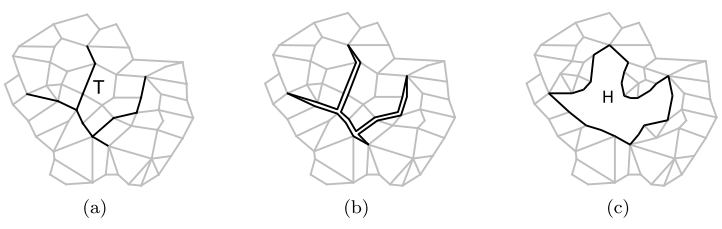
\includegraphics[scale=0.7]{imgs/cut_graph_example.png}
    \caption {Example of cutting process using a subgraph \(T\) to form a face \(H\) inside the graph. (\cite{Borradaile2012}).}
    \label{fig:cut_graph_example}
\end{figure}

% It is worth mentioning that if the subgraph used to do the cutting has cycles, the cutting process may disconnect components of the original graph.

From that, we define a \textbf{cut graph} \(CG\) as a subgraph of \(G\) that when used to cut \(G\) results in a planar graph.

The goal of this section is to find a \textbf{cut graph} \(CG\) of \(G\) that contains all terminals and whose cost is bounded by a constant times \(\opt\). Cutting \(G\) using \(CG\) results in a planar graph with a cycle \(\sigma\) as the boundary, where \(\sigma\) is twice the cost of \(CG\).

Figure~\ref{fig:mortar5} illustrates the process of cutting a graph of genus greater than 0.  Figure~\ref{fig:mortar5}(a) shows a cut graph drawn on a torus, while Figure~\ref{fig:mortar5}(b) shows the result of cutting the surface along the graph: the shaded area is homeomorphic to a disk, and the light area is the additional face of the planarized surface.

\begin{figure}[h]
    \centering
    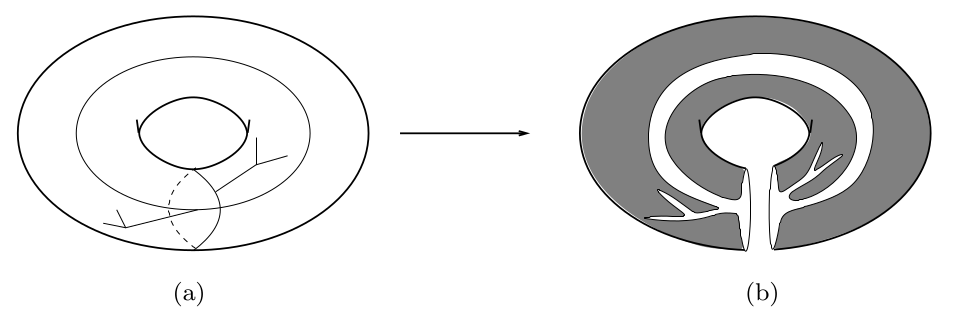
\includegraphics[scale=0.45]{imgs/mortar5.png}
    \caption {Example of a cut in a graph with \textit{genus} greater than zero. (\cite{Borradaile2012}).}
    \label{fig:mortar5}
\end{figure}


\cite{Borradaile2012} observed that, given a planar graph \(G\) and a spanning tree \(T\) of \(G\), the set of edges \(E(G) - E(T)\) induces a spanning tree \(T^{\star}\) in the dual graph \(G^{\star}\). Furthermore, if \(T\) is a minimum spanning tree of \(G\), then \(T^{\star}\) is a maximum spanning tree of \(G^{\star}\). This result was derived by \citeauthor{Borradaile2012} from the Lemma~1 of~\cite{EPPSTEIN199233}.

The result can be generalized for bounded \textit{genus} graphs: if \(T\) is a minimum spanning tree of \(G\) and \(T^{\star}\) is a maximum spanning tree of \(G^{\star} - E(T)\), then \(T^{\star}\) is a maximum spanning tree of \(G^{\star}\) and the size of the set of remaining edges \(X := E(G) - E(T) - E(T^{\star})\) is \(g\), or the Eulerian \textit{genus} of \(G\), obtained by Euler's formula. \cite{Eppstein} define such a triple \((T, T^{\star}, X)\) as the \textit{tree-cotree decomposition} of \(G\), and shows that a cut graph can be generated from this decomposition.

\begin{figure}[H]
    \centering
\begin{tikzpicture}


    \Vertex[x=0, y=2, color=white, Math,IdAsLabel]{A}
    \Vertex[color=white, Math,IdAsLabel]{B}

    \Vertex[x=1, y=1, color=white, Math,IdAsLabel]{C}
    \Vertex[x=2, y=0, color=white, Math,IdAsLabel]{D}

    \Vertex[x=1, y=-0.3, color=white, Math,IdAsLabel]{E}
    \Vertex[x=2, y=1.5, color=white, Math,IdAsLabel]{F}

    \Vertex[x=3, y=0, color=white, Math,IdAsLabel]{G}
    \Vertex[x=3, y=1.5, color=white, Math,IdAsLabel]{H}

    \Edge[opacity=1.0](A)(B)
    \Edge[opacity=0.3](A)(F)
    \Edge[opacity=1.0](A)(C)
    \Edge[opacity=1.0](C)(F)
    
    \Edge[opacity=0.3](A)(E)
    \Edge[opacity=1.0](C)(E)
    \Edge[opacity=0.3](D)(E)


    \Edge[opacity=0.3](F)(H)
    \Edge[opacity=0.3](H)(G)
    \Edge[opacity=0.3](G)(D)
    \Edge[opacity=0.3](D)(F)
    \Edge[opacity=0.3](F)(G)
    \Edge[color=green](D)(H)

    \Edge[color=red](F)(H)
    \Edge[color=red](F)(D)
    

\end{tikzpicture}
    \caption{Example of \(loop(T, e)\). The tree \(T\) is rooted at the vertex \(F\) and is represented by the black (non-opaque) edges. The edge \(e\) is represented in green and the paths between \(e\) and the vertex \(F\) are displayed in red. The \(loop(T, e)\) is composed of the union of the red and green edges.}
    \label{fig:loop_T_e}
\end{figure}


Let \(T\) be a spanning tree rooted at a vertex \(r\), and let \(e\) be an edge not contained in \(T\). We say that \(loop(T, e)\) is the simple cycle formed by \(e\) and the paths between \(r\) and both ends of \(e\) (exemplified in Figure~\ref{fig:loop_T_e}). Based on the results from \citeauthor{Eppstein},~\cite{Borradaile2012} showed in the following result.

\begin{flemma}[\cite{Borradaile2012}, Lemma 1]
    Given a tree-cotree decomposition \((T, T^{\star}, X)\), \(\{loop(T, e): e \in X\}\), induces a cut graph.
\end{flemma}

The construction of the cut graph for our purposes follows from~\cite{Borradaile2012}, with slight technical changes. We start with \(T_i\), which is a minimum spanning tree of the component \(C_i\) calculated in Algorithm~\ref{algorithm:pc-partition}, and contract it to a vertex \(r\).

We then find a shortest-path tree \(SPT\) rooted at \(r\), uncontract \(r\) back into \(T_i\) and set \(T := T_i \cup SPT\), where \(T\) is a spanning tree of \(G\). With that, we can then find a spanning tree \(T^\ast\) of \(G^\ast - E(T)\) using the results presented above.

Let \(X := E(G) - E(T) - E(T^\ast)\). As the output cut graph we return \(CG := T_i \cup \{loop(T, e): e \in X\}\).

We proceed to cut \(G\) using \(CG\) and duplicate each edge and vertex of \(CG\), thus, generating a cycle \(\sigma\) internal to \(CG\). After this process, let \(G_1\) be the planar graph obtained from \(G\). Finally, we invert the face \(\sigma\) in such a way that \(\sigma\) becomes the new external face of \(G_1\). From construction and Theorem~\ref{theoremClustering}, \(c(\sigma)\) is at most \(c \opt\) where \(c\) is a constant.

\citeauthor{Borradaile2012} refers to the algorithm presented above as \textbf{Planarize algorithm} and formalizes the result with the following lemma.

\begin{flemma}[\cite{Borradaile2012}, Lemma 2]
    The algorithm \textbf{Planarize} returns a cut graph \(CG\) such that cutting \(G\) open along \(CG\) results in a planar graph \(G_p\) with face \(f_\sigma\) whose facial walk \(\sigma\)

    \begin{enumerate}
        \item is a simple cycle,
        \item contains all terminals (some terminals might appear more than once as multiple copies might be created during the cutting process); and
        \item has cost \(c(\sigma) \leq c \opt\) for \(c > 0\) constant.
    \end{enumerate}
\end{flemma}

\subsubsection{Strips}

To continue with the algorithm, we need to present the following definition. Given $\epsilon > 0$ and a graph \(G\), a path \(P\) in \(G\) is \(\epsilon\)-\textit{short} if in each pair of vertices \((x, y) \in P\) the distance between \(x\) and \(y\) in \(P\) is at most \((1 + \epsilon)\) times the distance \(x\) and \(y\) in \(G\), in other words, \(dist_P(x, y) \leq (1 + \epsilon) dist_G(x, y)\).

We proceed to decompose the planar graph \(G_1\) into \textit{strips}. Let \(x\) and \(y\) be two vertices in \(\sigma\). Let \(\sigma[x, y]\) be the path between \(x\) and \(y\) in \(\sigma\) in the counterclockwise direction of the \textit{planar embedding} of \(G_1\) into a sphere. If \(x = y\), by convention \(\sigma[x, y] = \sigma\).

In order to segment \(G_1\) into strips, we find vertices \(x\) and \(y\) in \(\sigma\) such that \(\sigma[x, y]\) is the shortest path of \(\sigma\) which is not \(\epsilon\)-\textit{short} in \(\sigma\). Such a pair of vertices always exists since \(\sigma[x, y]\), with \(x = y\), is not \(\epsilon\)-\textit{short}. Let \(N\) be the shortest path between \(x\) and \(y\) in \(G_1\). Certainly \(c(N) < c(\sigma[x, y])\). We call \textbf{strip} the subgraph of \(G_1\) covered by \(N \cup \sigma[x, y]\). This process is performed recursively on the subgraph of \(G_1\) covered by \(N \cup (\sigma - \sigma[x, y])\). As a result, we have \(G_1\) segmented by strips. Items~(a) and (b) of Figure~\ref{fig:mortar2} illustrate this process.

\begin{flemma}[\cite{klein2006}, inequality (10)] \label{strip_length}
The total cost of the boundary of all strips is at most \((\frac{1}{\epsilon} + 1)\) times the cost of \(\sigma\).
\end{flemma}

\citeauthor{klein2006} also showed that the strip decomposition of a planar graph with \(n\) vertices can be found in time \(\mathcal{O}(n \log n)\).

Given a fixed strip, we denote \(N\) as the north-boundary of the strip and \(S\) as the south-boundary.

With the graph \(G_1\) decomposed into strips, as illustrated in Item~(b) of Figure~\ref{fig:mortar2}, the next step is, for each strip, to calculate the shortest paths, called \textit{columns}. Consider a strip with north and south boundaries, \(N\) and \(S\) respectively. We select vertices \(s_0, s_1, \dots\) in \(S\) as follows. We embed the north strip above the south strip, directing \(S\) and \(N\) from left to right. Let \(s_0\) be the leftmost vertex common to \(S\) and \(N\). By convention, the column \(C_0\) is defined as the shortest path between \(s_0\) and \(N\), in this case, an empty path.

For \(i \geq 1\), find the first vertex in \(S\) (from left to right) such that the cost of the path from \(s_{i-1}\) to \(s_i\) in \(S\) is greater than \(\epsilon\) times the cost of the shortest path from \(s_i\) to \(N\) within the strip, that is, \(dist_S(s_{i-1}, s_i) > \epsilon \cdot dist_{strip}(s_i, N)\). Thus, column \(C_i\) is defined as the shortest path between \(s_i\) and \(N\) in the strip, as illustrated by Item~(c) of Figure~\ref{fig:mortar2}.

\begin{figure}[H]
    \centering
    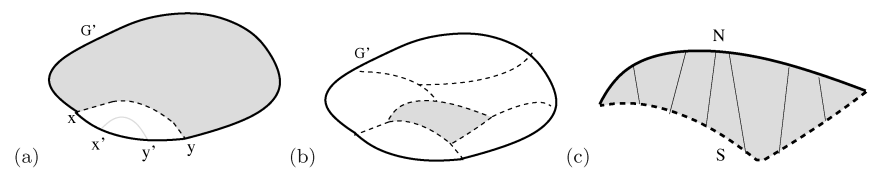
\includegraphics[scale=0.5]{imgs/mortar2.png}
    \caption{Construction of strips in Mortar Graph (\cite{Borradaile2009b}).}
    \label{fig:mortar2}
\end{figure}

In Figure~\ref{fig:mortar2}, Item~(a) shows the first track is created by a path (dashed) connecting \(x\) and \(y\). The distance between every pair of vertices \(x'\) and \(y'\), between \(x\) and \(y\) on the boundary, is well approximated by the distance on the boundary. We use recursion in the shaded area; Item~(b) shows how a graph is divided into bands (by the dashed lines). A strip is increased in Item~(c). Columns (vertical lines) are taken from the set of shortest paths between the ``low'', or south boundary (dashed line) and the ``up'', or north boundary (solid line).

\begin{flemma}[\cite{klein2006}, Lemma 5.2]
The sum of all column costs in a strip is at most \(\epsilon^{-1} \cdot c(S)\).
\end{flemma}

After having the columns calculated, for each strip, we have a set \(C_0, C_1, \dots, C_s\) of columns of the strip.

For \(\epsilon > 0\), let \(\kappa = \kappa(\epsilon) = 4 \epsilon ^ {-2} (1 + \epsilon ^ {-1})\). We will use this constant on the following definition and for the following lemmas due to \cite{Borradaile2009b}.

% Let \(\mathcal{C}_i = C_i \cup C_{i+\kappa} \cup C_{i+2\kappa} \cup \dots\) for \(i \in \{0, 1, \dots, \kappa - 1\}\).
Let \(\mathcal{C}_i = \bigcup_{j=0}^{\kappa-1} C_{i+j\kappa}\) for \(i \in \{0, 1, \dots, \kappa - 1\}\).

Let \(i^\ast\) be the index that minimizes \(c(\mathcal{C}_i)\). We designate the columns of \(\mathcal{C}_i^\ast\) as \textbf{super-columns}.

\begin{flemma}[\cite{Borradaile2009b}, Lemma 6.5]
The sum of the costs of the super-columns in a strip is at most \(\kappa^{-1}\) times the sum of the costs of the columns in the strip.
\end{flemma}

\begin{flemma}[\cite{Borradaile2009b}, Lemma 6.6] \label{borradaile_2009b_lemma_6_6}
     The sum of the costs of all the super-columns over all strips is at most \(c \epsilon \opt\), where \(\epsilon > 0\) and \(c > 0\) depends on \(\epsilon\).
\end{flemma}

We define as the \textbf{Mortar Graph} \(MG\) of \(G\) the embedded planar subgraph generated by the edges of \(T_i\), the edges of the strips, and the edges of super-columns. This is illustrated in Item~(b) of Figure~\ref{fig:mortar3}.

We note two properties derived from the results presented during the construction of \(MG\). First, let \(Q\) be the set of all terminals of \(G\), by construction, we have that \(Q \subseteq V(MG)\). The second property is presented below.

\begin{flemma} \label{length_mg}
     \(c(MG) \leq k \epsilon c(\sigma)\) with \(k > 0\) constant.
\end{flemma}
\begin{proof}
    The result follows from Theorem~\ref{theoremClustering} and Lemmas~\ref{strip_length} and~\ref{borradaile_2009b_lemma_6_6}.
\end{proof}

\subsubsection{Bricks}

To create a \textbf{brick} (illustrated in  Figure~\ref{fig:mortar3}(c)), for each face \(f\) of \(MG\), we duplicate the border edges and vertices of \(f\). This results in a disconnected induced subgraph of \(G_1\) that is entirely contained within the ``external'' copy of \(f\)'s border (Figure~\ref{fig:mortar4}(c)). The result of this process can be seen in Figure~\ref{fig:mortar4}.

Figure~\ref{fig:mortar4}(a) illustrates the boundary of a face \(f\) of \(MG\) as a cycle of edges (thick edges), possibly with repetition (that is, an edge can occur twice at the border). The light edges are those inside \(f\) in \(G\). Figure~\ref{fig:mortar4}(b) shows an example of brick \(B\) obtained by the process described above. \(B\) has boundary \(\partial B\). Figure~\ref{fig:mortar4}(c) shows a brick \(B\) contained within the ``external'' copy of the border of \(f\).

\begin{figure}[h]
    \centering
    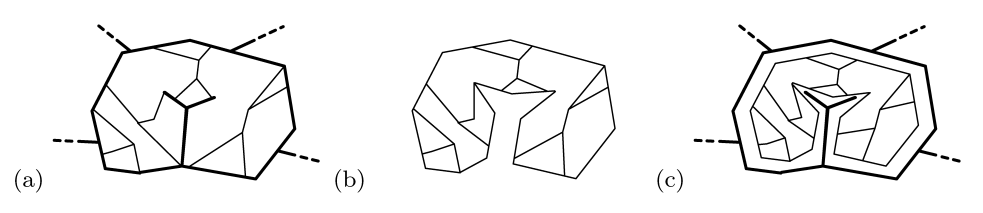
\includegraphics[scale=0.45]{imgs/mortar4.png}
    \caption{Construction of a brick. (\cite{Borradaile2009b}).}
    \label{fig:mortar4}
\end{figure}

The boundary \(\partial B\) of a brick \(B\) is the simple cycle formed by the edges of the boundary. The corresponding face of \(MG\) is called \textbf{mortar boundary} from~\(B\). Each edge of \(MG\) occurs at most in the disjoint union of the boundary of the bricks.

\begin{flemma}[\cite{Borradaile2009b}, Lemma 6.10]
    A mortar boundary \(B\), in counterclockwise order, is the concatenation of four paths \(W\), \(S\), \(E\), \(N\) (west, south, east, north) such that:
    \begin{enumerate}
        \item The set of edges \(B - \partial B\) is nonempty.
        \item Every vertex of \(\mathcal{D} \cap B\) is in \(N\) or in \(S\).
        \item \(N\) is \(0\)-short in \(B\), and every proper subpath of \(S\) is \(\epsilon\)-short in S.
        \item There exist \(k \leq \kappa\) vertices \(s_0, s_1, s_2, \dots, s_k\) ordered from west to east along \(S\) such that, for any vertex \(x\) of \(S[s_i, s_{i+1})\), the distance from \(x\) to \(s_i\) along \(S\) is less than \(\epsilon\) times the distance from \(x\) to \(N\) in \(B\), that is, \(dist_S(x, s_i) < \epsilon dist_B(x, N)\).
    \end{enumerate}
\end{flemma}

\subsubsection{Portals}

The connection between a face \(f\) of \(MG\) and its respective brick \(B\) is performed through a subset of vertices of \(\partial B\) called \textbf{portals}. This connection is made in such a way that, for each portal \(p\) of \(\partial B\), an edge with weight 0 is placed between \(p\) and the vertex of which it was duplicated in \(\partial f\).

For each brick \(B\), we set some vertices of \(\partial B\) as \textbf{portals}. We define \(\theta = \theta(\epsilon) = 18 \cdot \alpha(\epsilon) \cdot \epsilon ^ {-2}\). Where \(\alpha(\epsilon)\) is a constant that will be defined later.

For portal selection, we use the following greedy algorithm. An initial vertex \(v_0\) of \(\partial B\) is selected with uniform probability. Then we define \(v_1\) as the first vertex of \(\partial B\) clockwise such that \(c(\partial B[v_0, v_1]) > c(\partial B) / \theta\). This process is repeated for \(v_i\) in \(\partial B\) until \(v_0 \in V(\partial B (v_{i-1}, v_i))\).

Using the previous construction, we get the following properties given by \cite{Borradaile2009b}.

\begin{flemma}[\cite{Borradaile2009b}, Lemma 7.1] \label{lemma:cobertura}
(Cover property): For any vertex \(x \in \partial B\), there exists a portal \(y\) such that the \(x\)-to-\(y\)-subpath of \(\partial B\) has a maximum cost \(c(\partial B) / \theta\).
\end{flemma}

\begin{flemma}[\cite{Borradaile2009b}, Lemma 7.2]
(Cardinality property): There are at most \(\theta\) portals in \(\partial B\).
\end{flemma}

With that, we have a Mortar Graph \(MG\) with a set of bricks connected with the face boundaries of \(MG\) through portal edges, as illustrated by Item~(d) Figure~\ref{fig:mortar3}. This construction is named by \citeauthor{Borradaile2009b} as \textbf{portal-connected graph}, and is denoted as \(\mathcal{B}^{+}(MG)\).

\begin{figure}[H]
    \centering
    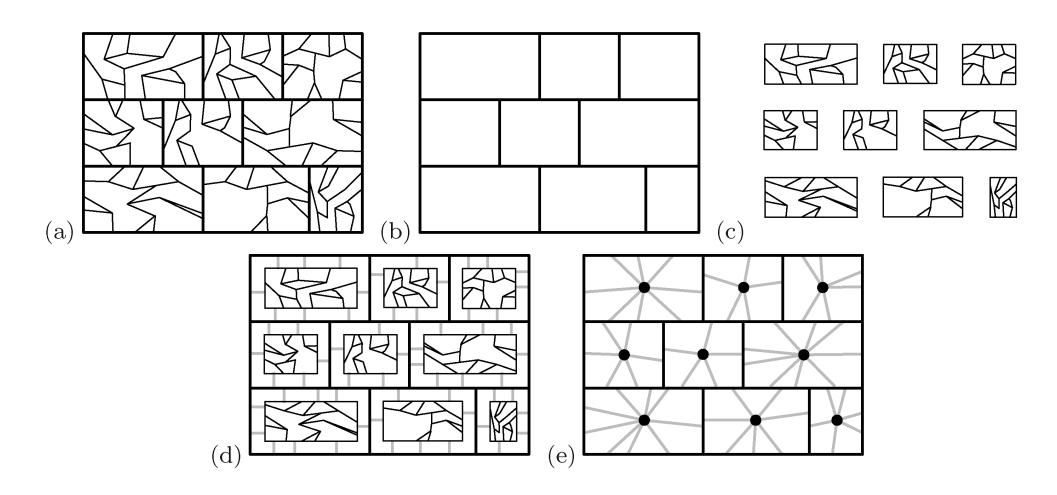
\includegraphics[scale=0.4]{imgs/mortar3.png}
    \caption{Mortar Graph. (\cite{Borradaile2009b}).}
    \label{fig:mortar3}
\end{figure}

Figure~\ref{fig:mortar3} shows in Item~(a) the graph \(G_1\), highlighting the edges of the Mortar Graph. 
Item~(b) shows only the Mortar Graph \(MG\) obtained. 
Item~(c) shows the set of bricks corresponding to \(MG\) (those will be defined ahead). 
Item~(d) illustrates a portal-connected graph \(\mathcal{B}^{+}(MG)\) (will be presented ahead), where the portal edges are gray. 
Item~(e) shows \(\mathcal{\mathcal{B}}^{+}(MG)\) with the bricks contracted into vertices, resulting in \(\mathcal{B}^{\div}(\mathcal{B }^{+}(MG))\).

\subsection{Spanner construction}

Finally, we proceed to prove Theorem~\ref{theorem:spanner}.

We start by building a separate subgraph \(H_i\) for each \(T_i\). Let \(H_i\) be a Mortar Graph created from \(T_i\). Following that, for each brick \(B\) and a selection of its portals \(\Pi' \subseteq \Pi\), we add to \(H_i\) an optimal Steiner Tree that reaches \(\Pi'\) and uses only edges from the interior of \(B\) or its boundary. This can be done in polynomial time in \(\theta\) using the algorithm proposed in \cite{ericksonST}, since all terminals lie on the infinite face of a planar graph.

Note that for fixed \(\epsilon\) and \(g\) there is at most a constant number of portals, hence a constant number of such Steiner Trees, and the cost of each is at most the cost of the boundary of the brick \(B\).

We will leverage an auxiliary result to prove both spanner properties.

\begin{flemma}\label{lemma:borradaile_10_1}
    Let \(G\) be a planar embedded graph and let \(C\) be a subgraph of \(G\) that intersects a \(\epsilon\)-short path \(P\). There is a subpath of \(P\) spanning the vertices of \(C \cap P\) whose total cost is \((1 + \epsilon) c(C)\)
\end{flemma}
\begin{proof}
    Let \(P'\) be the shortest subpath of \(P\) that spans all the vertices of \(C \cap P\). There is a path \(Q\) in \(C\) that connects all vertices of \(C \cap P\). Since \(P\) is \(\epsilon\)-short \(c(P') \leq (1 + \epsilon)c(Q) \leq (1 + \epsilon)c(C)\).
\end{proof}

\begin{flemma} [\cite{Bateni}, Lemma 4.1] \label{bateni_4_1_forest}
    For any forest \(F\) in a brick \(B\), there exists a forest \(F'\) such that
\begin{enumerate}
    \item \(c(F') \leq (1 + \epsilon)c(F)\);
    \item \(F'\) crosses the boundary of \(B\) at most \(\alpha\) times; and
    \item any two vertices on \(N\)- or \(S\)-boundaries of \(B\) connected by \(F\) are also connected by \(F'\)
\end{enumerate}
\end{flemma}

In Corollary~\ref{bateni_4_1_multicycle}, we will generalize the result above to a collection of cycles (instead of a forest), but first, we need to introduce the concept of \textbf{cleaving}.

Put simply, cleaving is the process of breaking a vertex into two new vertices and adding an artificial, zero-cost edge between them. It can be formalized as: given a vertex \(v\) and a bipartition \(A, B\) of the edges incident to \(v\), split \(v\) into two new vertices \(v_A\) and \(v_B\). Then, connect the endpoints of the edges in \(A\), previously connected to \(v\), to \(v_A\), and the edges in \(B\) to \(v_B\). Finally, add a zero-cost edge \(e_{AB}\) between \(v_A\) and \(v_B\). This operation is illustrated in Figure~\ref{fig:cleaving} (a) and (b).

There can be two types of cleaving:
\begin{itemize}
    \item Simplifying Cleaving (Figure~\ref{fig:cleaving} (c) and (d)). Let \(C\) be a clockwise, non-self-crossing (i.e., planar) non-simple cycle that visits a vertex \(v\) twice. Defined a bipartition of the edges incident to \(v\) as follows: given the clockwise embedding of the edges incident to \(v\), let \(A\) start and end with consecutive edges of \(C\) and contain only two edges of \(C\), let \(B\) be the remaining edges. Such a bipartition exists because \(C\) is non-self-crossing.
    \item Lengthening Cleaving (Figure~\ref{fig:cleaving} (e) and (f)). Let \(C\) be a simple cycle, and let \(v\) be a vertex on \(C\) with two edges \(e_A\) and \(e_B\) adjacent to \(v\) embedded strictly inside \(C\), and let \(e'_A\) and \(e'_B\) be consecutive edges of \(C\) adjacent to \(v\) such that the following bipartition is non-crossing concerning the embedding: \(A\), \(B\) is a bipartition of the edges adjacent to \(v\) such that \(e_A, e'_A \in A\) and \(e_B, e'_B \in B\).
\end{itemize}

\begin{figure}[h]
    \centering
    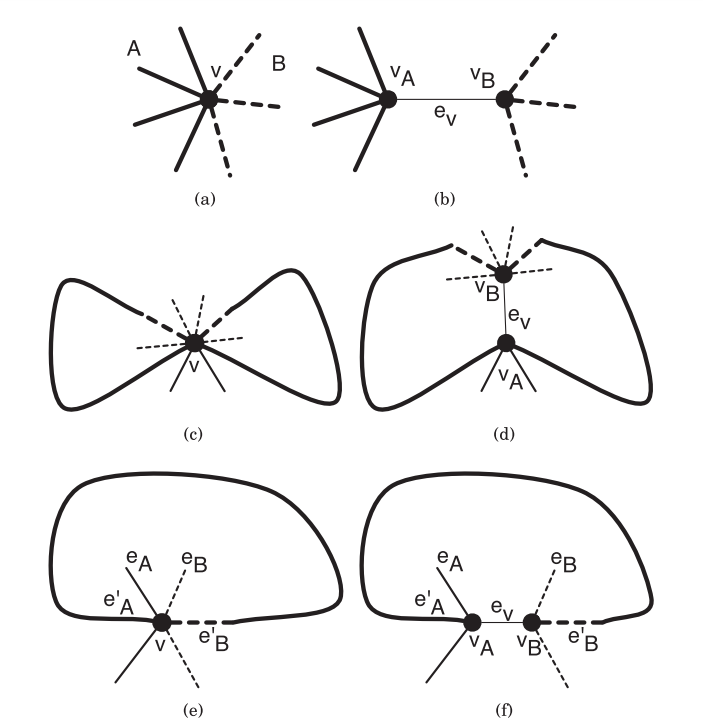
\includegraphics[scale=0.5]{imgs/cleaving.png}
    \caption{Cleavings illustrated (\cite{borradaile_2EC}).}
    \label{fig:cleaving}
\end{figure}

\begin{fcorollary}\label{bateni_4_1_multicycle}
For any collection of cycles \(M\) in a brick \(B\), there is a collection of cycles \(M'\) such that
\begin{enumerate}
    \item \(c(M') \leq (1 + c \epsilon)c(M)\)
    \item \(M'\) crosses the boundary of \(B\) at most an \(\alpha\) (constant) number of times
    \item any two vertices on \(N\)- or \(S\)-boundaries of \(B\) connected by \(M\) are also connected by \(M'\)
\end{enumerate}
\end{fcorollary}
\begin{proof}
    Let \(M^\ast\) be an optimal solution to the SMCP in \(G\) and let \(MG\) be a Mortar Graph built from \(G\). 

    For a given brick \(B\) (with \(W, N, E, S\) boundaries), let \(M\) be the intersection between \(M^\ast\) and \(B\). Note that \(M\) might be composed of cycles and trees (e.g., cycle fragments that connect to themselves outside the brick) and each vertex in \(M \cap \partial B\).

    We begin the construction of \(M_1\) by adding the \(W\) and \(E\) boundaries of \(B\) to \(M\). We know from Lemma~\ref{borradaile_2009b_lemma_6_6} that the cost of the union of \(M^\ast\) with all super-columns (i.e., the west and east boundaries of all bricks) is at most \((1 + 2 c \epsilon) \opt\).

    To streamline the rest of the proof, we perform the simplifying cleaving on non-simple cycles of \(M_1\) until all cycles become simple (also accounting for duplicated edges).
    We can have two situations for each component \(C\) of \(M_1\):
    \begin{enumerate}
        \item \(C\) connects vertices in \(N\) or vertices in \(S\)
        \item \(C\) connects vertices from \(N\) and \(S\)
    \end{enumerate}

    To tackle case (1), we use Lemma~\ref{lemma:borradaile_10_1} to replace the path of \(C\) that connects two vertices in \(N\) with a subpath of \(N\), which connects the same vertices. Since \(N\) is a \(\epsilon\)-path, the Lemma holds, and the increase in cost is limited by a \((1 + \epsilon)\) factor.

    For case (2), we apply the lengthening cleaving to the boundary of brick \(B\). For each vertex \(v\) in \(M_1 \cap \partial B\) that has a degree greater than one, we perform the lengthening cleaving in \(v\). We repeat this process while there are still multiple edges of the solution embedded in a brick that is incident to a shared boundary vertex. In other words, we have that the intersection of \(M_1\) with the interior of brick \(B\) is a subgraph whose joining vertices with \(\partial B\) have degree one.


    The first property follows, since - as mentioned - in case (1), the increase in cost is limited by a \((1 + \epsilon)\) factor, and in case (2) we only add zero-cost edges.
    
    To get the second and third properties, we can directly apply Lemma~\ref{bateni_4_1_forest} (Structural properties of Bricks) on \(M_1\). 
\end{proof}

Considering the final spanner \(H\) to be the union of all \(H_i\)'s, we proceed to prove that \(H\) indeed respects both properties of \textbf{quasi-optimality} and \textbf{shortness}.

\begin{flemma}{{(Shortness property).}}\label{spanner_shortness_property} Given a graph \(G\) and a subgraph \(H\) of \(G\) constructed with the process above, the cost of \(H\) is at most \(f(\epsilon, g) \opt\) for a certain function
\(f(\epsilon, g)\).
\end{flemma}
\begin{proof}
Note that each \(H_i\) is constructed from \(MG_i\) (which by its turn is built from \(T_i\)), a set of portal edges connected to \(MG_i\), and a limited set of Steiner Trees inside the bricks. By Lemma~\ref{length_mg}, \(c(MG_i) \leq f(\epsilon, g) c(T_i)\). For each brick \(B\), we add at most \(2^{\theta}\) trees, each with cost no more than \(c(\partial B)\). Since each edge of \(MG_i\) may appear in at most two bricks, the total cost is bounded by \(2^{\theta + 1} c(MG_i)\). Therefore, \(c(H_i) \leq 2^{\theta + 1} c(MG_i) = f(\epsilon, g) c(T_i)\).

By Theorem~\ref{theoremClustering}, the sum of the cost of all \(T_i\) is no more than \((16/\epsilon + 4) \opt_{\mathcal{D}}(G_{in})\).
This implies that the sum of the cost of all \(H_i\) is no more than \(f(\epsilon, g) (16/\epsilon + 4) \opt_{\mathcal{D}}(G_{in})\).
\end{proof}

\begin{flemma}\label{spanner_quasi_optimality_property}
    Quasi-optimality property.~\(\opt_{\mathcal{D}}(H) \leq (1 + c \epsilon) \opt_{\mathcal{D}}(G_{in})\) with \(c\) and \(\epsilon\) constants.
\end{flemma}
\begin{proof}

    Let \(\{C_i\}_{i=1}^k\) be the set of components outputted by Algorithm~\ref{algorithm:pc-partition}.

    From Theorem~\ref{theoremClustering}, we have that \(\sum_{i}^k \opt_{\mathcal{D}_i} \leq (1 + \epsilon) \opt_{\mathcal{D}}\). So we can focus on proving that \(\opt_{\mathcal{D}_i}(H_i) \leq (1 + c \epsilon) \opt_{\mathcal{D}_i}(G_{in})\).

    Consider each \(H_i\) as formed in the process above, so each \(H_i\) is formed by a Mortar Graph built using \(T_i\) (a minimum spanning tree of \(C_i\) from Theorem~\ref{theoremClustering}), the portal edges and the set of Steiner Trees connecting the portals in each Brick.

    Let \(M^\ast_i\) be an optimal solution for the SMCP considering \(\mathcal{D}_i\), i.e. \(c(M^\ast_i) = \opt_{\mathcal{D}_i}(G_{in})\). We add the set of all super-columns in \(H_i\) to \(M^\ast_i\) to get \(M^1_i\). Recall that, by Lemma~\ref{borradaile_2009b_lemma_6_6}, the cost of these super-columns is at most \(c \epsilon \opt_{\mathcal{D}_i}(G_{in})\).

    Next, we replace the intersection of \(M_i^1\) and each brick with another subgraph having the properties of  Corollary~\ref{bateni_4_1_multicycle}. Let \(M_i^2\) be the new subgraph. The cost of the solution increases to no more than a \(1 + c \epsilon\) factor.

    From  Corollary~\ref{bateni_4_1_multicycle}, we know that \(M_i^2\) crosses each brick at most \(\alpha\) times, so we can ensure that moving these intersection points to the portals adds no more than a constant factor in the cost.

    Consider a brick \(B\) with boundaries \(W, N, E, S\). Connect each intersection point of the brick to its closest portal. Each connection on a brick \(B\) moves by at most \(2 c(\partial B) / \theta\). Therefore, the total movement of each brick is at most \(\alpha 2 c(\partial B) / \theta\), which is no more than \(2 \epsilon^2 c(\partial B) / \gamma(\epsilon, g)\). Hence, the total additional cost for all bricks of \(H_i\) is bounded by \(4 \epsilon^2 c(T_i)\). Let \(M_i^3\) be the resulting subgraph.

    Hence the cost of \(M_i^3\) is at most \(4 \epsilon^2 c(T_i) + c(M_i^2)\). Considering that \(c(M_i^2) \leq (1 + \epsilon) c(M_i^1)\) and \(c(M_i^1) \leq \epsilon^2 c(T_i) + M^\ast_i\), we have that \(c(M_i^3) \leq 4 \epsilon^2 c(T_i) + (1 + \epsilon) c(M^\ast_i)  + \epsilon^2 c(T_i)\)

    Let \(M' = \bigcup_i^k M_i^3\). Accounting that \(\sum_i^k c(T_i) \leq (4/\epsilon + 4) \opt\) (from Theorem~\ref{theoremClustering}), it holds that \[c(M') \leq \sum_i^k \left ( 4 \epsilon^2 c(T_i) + (1 + \epsilon) c(M^\ast_i)  + \epsilon^2 c(T_i) \right).\] 
    Therefore, we can conclude that  \(c(M') \leq (1 + 21 \epsilon + 20 \epsilon^2) \opt = (1 + c'\epsilon) \opt\).
\end{proof}


\section{PTAS for Graphs of Bounded Genus}
\label{section:ptas_bounded_genus}

We can now prove one of the main results of this work, which is a PTAS for the Steiner Multicycle Problem on graphs with bounded genus.

First, we state an auxiliary result from \cite{Demaine2010}.

\begin{ftheo}[\cite{Demaine2010} Theorem 1.1] \label{demaineResult}
    For a fixed genus \(g\), and any integer \(k \geq 2\) and for every graph \(G\) of Euler genus at most \(g\), the edges of \(G\) can be partitioned into \(k\) sets such that contracting the edges in any of the sets results in a graph of treewidth \(\mathcal{O}((g + 1)^2k)\). Furthermore, such a partition can be found in \(\mathcal{O}((g+ 1)^{5/2} n^{3/2} \log{n})\) time.
\end{ftheo}

The proposed PTAS algorithm is presented in Algorithm~\ref{smcp-ptas}.

\begin{algorithm}
\caption{SMCP-PTAS}
\label{smcp-ptas}
\begin{algorithmic}[1]

\Require Graph \(G_{in}\) of bounded genus \(g\), a set of terminal pairs \(\mathcal{D}\), and a constant \(1 \geq \epsilon > 0\).
\Ensure A collection of cycles satisfying \(\mathcal{D}\) whose cost is at most \((1 + c' \epsilon) \opt\)
\State  \(\epsilon' \gets \epsilon / 6\)
\State  \(k \gets \max\left \{ f(g, \epsilon')/{\epsilon'}, \: 2\right \}\); \(f(g, \epsilon')\) as in Lemma~\ref{spanner_shortness_property} \label{alg_smcp_ptas:k}
\State Construct a spanner \(H\) of \(G_{in}\) \label{alg_smcp_ptas:SpannerCall}
\State Use Theorem~\ref{demaineResult} to partition the edges of \(H\) into \(E_1, \dots, E_k\) \label{alg_smcp_ptas:partDemaine}
\State  \(j^\ast \gets \arg\min\limits_{j \in \{1,\ldots,k\}} c(E_j)\)
\State Find a \((1 + k \epsilon)\) collection of cycles (multiset of edges) \(M^\ast\) with respect to \(\mathcal{D}_i\) in \(H/E_{j^\ast}\) using Theorem~\ref{dynamicProgramming}, and with \(k\) constant \label{alg_smcp_ptas:dp}
\State \(M \gets M^\ast \cup E_{j^\ast}\)
\State \Return  \(M\)

\end{algorithmic}
\end{algorithm}

\begin{ftheo}
    The collection of cycles \(M\) produced by Algorithm~\ref{smcp-ptas} on input $(G_{in}, \mathcal{D})$ is a feasible solution for the SMCP and has cost at most \((1 + c' \epsilon) \opt\), with \(c'\) and \(\epsilon\) constants.
\end{ftheo}
\begin{proof}

    In the line~\ref{alg_smcp_ptas:SpannerCall} of Algorithm~\ref{smcp-ptas}, we construct a spanner \(H\) of \(G_{in}\), which respects the properties described in Lemma~\ref{spanner_quasi_optimality_property} and Lemma~\ref{spanner_shortness_property}, that is:

    \begin{itemize}
        \item \(c(H) \leq f(g, \epsilon) \opt\), with \(f(g, \epsilon)\) being a constant that depends on \(\epsilon\) and the genus \(g\) of \(G_{in}\);
        \item \(\opt_{\mathcal{D}}(H) \leq (1 + c \epsilon) \opt_{\mathcal{D}} (G_{in})\).
    \end{itemize}

    Note that Lemma~\ref{spanner_quasi_optimality_property} implies that there is a feasible solution for the SMCP contained in \(H\).

    In line~\ref{alg_smcp_ptas:partDemaine}, we proceed to partition \(H\) using Theorem~\ref{demaineResult}. We choose \(k\) such that \(k = \max( \frac{f(g, \epsilon)}{\epsilon}, 2)\) where \(f(g, \epsilon)\) is the constant from Lemma~\ref{spanner_shortness_property}. 
    
    From Lemma~\ref{demaineResult}, by splitting \(H\) into \(k\) edges sets, we have \(c(E_{j^\ast}) \leq \epsilon \opt\). Moreover, contracting \(E_{j^\ast}\) from \(H\) produces a graph of treewidth \(\mathcal{O}((g +1)^2 k)\).

    Before contracting \(H\) with \(E_{j^\ast}\), we need to do a small treatment of the terminals contained in \(E_{j^\ast}\). We create a new vertex for each terminal in \(E_{j^\ast}\) and connect it to the terminal with a new edge of cost zero. This new vertex will serve as a ``temporary'' terminal in \(H / E_{j^\ast}\). Note that this process does not increase the cost of the final solution, as all added edges have cost zero.

    In line~\ref{alg_smcp_ptas:dp} of Algorithm~\ref{smcp-ptas}, we can find a solution \(M^\ast\) in \(H / E_{j^\ast}\) via Theorem~\ref{dynamicProgramming} and Theorem~\ref{demaineResult}. The cost of \(M^\ast\) is at most \((1 + 2 \kappa \epsilon) \opt\), with \(\kappa = \kappa(\epsilon) = 4 \epsilon ^ {-2} (1 + \epsilon ^ {-1})\).

    Finally, we join the solution \(M^\ast\) with the edges in \(E_{j^\ast}\). To guarantee the feasibility of the union as a solution, we duplicate each edge in \(E_{j^\ast}\). Note that the cost of \(E_{j^\ast}\) accounting for the duplication is at most \(2 \frac{c(H)}{k}\), which equals \(2 \frac{f(g, \epsilon) c(G_{in})}{f(g, \epsilon) / \epsilon} = 2 \epsilon \cdot c(G_{in})\).

    From Theorem~\ref{dynamicProgramming}, we have that \(c(M^\ast) \leq (1 + 2 \kappa \epsilon \opt)\). So \(c(M^\ast \cup E_{j^\ast}) \leq (1 + (2 \kappa + 2) \epsilon) \opt\) holds, and by considering a constant \(c' = 2 \kappa + 2\), we have \(c(M) \leq (1 + c' \epsilon) \opt\).

\end{proof}

The running time of the algorithm, excluding the bounded treewidth PTAS, is bounded by \(\mathcal{O}(n^2 \log n)\). Moreover, the running time of the current procedure for solving bounded treewidth instances is bounded by a polynomial, where \(k\) and \(\epsilon\) appear in the exponent.

\chapter{Conclusion}
\label{chapter:conclusion}

In this work, we first proposed a polynomial-time approximation scheme (PTAS) algorithm to solve the Steiner Multicycle Problem (SMCP) on graphs of bounded \textit{genus}. 
This PTAS was built upon ideas from various sources such as \cite{Borradaile2009b}, \cite{Borradaile2012}, and \cite{Bateni}, which we adapted to the Steiner Multicycle Problem, particularly to the restricted version R-SMCP. 
As mentioned in the introduction, we can readily transform instances of SMCP into R-SMCP.
The modifications of the algorithm proposed by~\citeauthor{Bateni} were mainly to extend their definitions and techniques to cycles. 
In particular, it was necessary to adapt most proofs to guarantee that all vertices in the resulting graphs have even degree.   

We also implemented the 3-approximation algorithm proposed by \cite{smcp_3apx}, which was tested on the same instances previously used by \cite{Pereira2018TheSM}. 
% The algorithm was implemented in C++ using the Graph library \cite{lemon} and the Optimization library \cite{gurobi}.
The experimental results showed that the 3-approximation consistently outperformed the theoretical bounds of solution quality. However, the results were still inferior in both quality and running time when compared to the heuristic proposed by \cite{Pereira2018TheSM}.
One significant bottleneck in the algorithm's performance was the Gomory-Hu trees calculation on the 2-approximation for the SNDP, especially for larger instances.
We believe further improvements are possible, mainly by employing a more robust algorithm in the short-cutting step and by applying a better strategy to verify the flow between terminal pairs in the 2-approximation for the SNDP step.
In particular, for practical implementations, it might be worth considering using a heuristic instead of the 2-approximation in the SNDP step of the algorithm. This heuristic could significantly improve the algorithm's performance, despite loosing theoretical guarantees of the quality of the solutions.

For future works, we propose expanding the PTAS for bounded-genus graphs algorithm to encompass a more diverse class of graphs, such as H-minor-free graphs. A possible path to achieve this is to use a nearly light subset \((1 + \epsilon)\)-spanner as proposed by \cite{light_spanners_tsp}.

% implementar a aproximação
Another research direction is to implement the proposed PTAS and carry out computational experiments, as \cite{TazariLargeConstants} and \cite{implementationPTASeuclidianTSP} proposed for the Steiner Tree and Euclidean TSP problems, respectively.


% \chapter{Introdução}

% Segundo \cite{horn86robot}, todo triângulo equilátero tem os lados iguais. Já
% segundo \cite{shashua97photometric}, todo quadrado também tem.

% Veja que o pacote \verb|natbib| permite uma série de formas diferentes para
% fazer referências bibliográficas. O comando padrão, \verb|\cite|, realiza a
% citação comum vista no parágrafo anterior. Outros comandos permitem, por
% exemplo, citar somente o autor --- por exemplo, citar o trabalho de
% \citeauthor{samaras99coupled} --- ou colocar automaticamente a citação entre
% parênteses \citep{hougen93estimation, sato99illumination2, sato99illumination1,
% sato01stability}. Os comandos usados foram, respectivamente, \verb|\citeauthor|
% e \verb|\citep|. Veja a documentação do \verb|natbib| na Internet para conhecer
% outros comandos e exemplos de uso.

% Citações aleatórias para fazer com que as referências bibliográficas ocupem
% mais de uma página: \cite{bichsel92simple, dror01statistics, guisser92new}.


% \section{Motivação}

% \dummytxtb\dummytxta

% \subsection{Sub-motivação}


% \dummytxtc\dummytxtb

% \subsection{Mais uma sub-seção}

% \dummytxta\dummytxtc

% \subsubsection{Descendo mais um nível}

% \dummytxtb\dummytxta


% \chapter{Desenvolvimento}

% \dummytxtb\dummytxta\dummytxtc

% \begin{figure}[h]
%     \centering
%     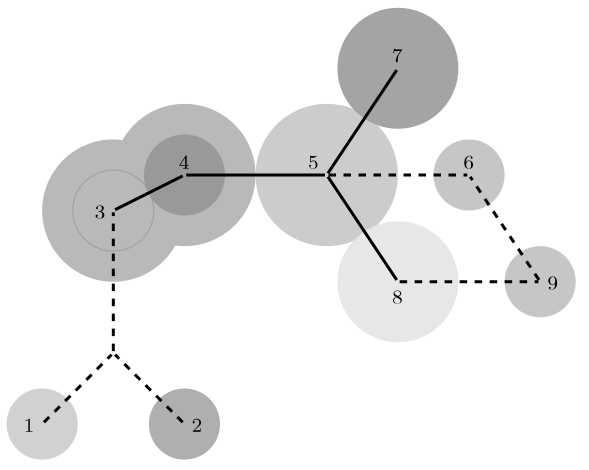
\includegraphics[scale=0.6]{imgs/clustering.png}
%     \caption{Uma figura de exemplo.}
%     \label{fig:exemplo}
% \end{figure}

% \dummytxtb\dummytxta\dummytxtc\dummytxtb

% \begin{table}[t]
%     \caption{Uma tabela de exemplo.}
%     {\centering
%     \begin{tabular}{lcr} \toprule
%     \emph{Left-aligned} & \emph{Centered} & \emph{Right-aligned} \\ \midrule
%     Lorem ipsum & dolor sit & amet \\
%     consectetur adipisicing & elit, sed do eiusmod & tempor \\
%     incididunt ut & labore et dolore & magna aliqua. \\ \bottomrule
%     \end{tabular}\par
%     }
% \end{table}


% Aqui vem a parte da bibliografia: use o comando \ppgccbibliography indicando
% apenas o nome do arquivo .bib (sem a extensão).
\ppgccbibliography{bibfile}


% Este comando encapsula o conjunto de apêndices. A sua função é fazer com que
% a numeração dos apêndices seja feita com letras maiúsculas (A, B, C, etc.) e
% a palavra "Apêndice" anteceda as entradas no Sumário.
% \begin{appendices}

% % Para cada apêndice, um \chapter
% \chapter{Um apêndice}

% \dummytxta
% \dummytxtb
% \dummytxtc
% \dummytxta
% \dummytxtb

% \chapter{Outro apêndice}

% \dummytxta
% \dummytxtb
% \dummytxtc
% \dummytxta
% \dummytxtb

% % Fim dos apêndices (usar apenas depois do último apêndice)
% \end{appendices}


% Este comando encapsula o conjunto de anexos. A sua função é fazer com que a
% numeração dos anexos seja feita com letras maiúsculas (A, B, C, etc.) e a
% palavra "Anexo" anteceda as entradas no Sumário.
% \begin{attachments}

% % Para cada anexo, um \chapter
% \chapter{Um anexo}

% \dummytxta
% \dummytxtb
% \dummytxtc
% \dummytxta
% \dummytxtb

% \chapter{Outro anexo}

% \dummytxta
% \dummytxtb

% % Fim dos anexos (usar apenas depois do último anexo)
% \end{attachments}


\end{document}